% How accurate LIGHT_Kr v0_4 is: the pure-krypton model, scored against
% pure-krypton measurements, with its propagated uncertainty, its
% reference point and its checks. No number here is typed by hand except
% the measurements, which carry their sources. They come from
%   overview_v0_4_numbers.tex     make_overview_v0_4.py     (\wg)
%   system_map_v0_4_numbers.tex   make_system_map_v0_4.py   (\wm)
% Build from LIGHT_Kr/docs:
%   python3 make_system_map_v0_4.py && python3 make_overview_v0_4.py
%   latexmk -pdf accuracy_overview_v0_4.tex
\documentclass[11pt]{article}
\usepackage[a4paper,margin=2.2cm]{geometry}
\usepackage[T1]{fontenc}
\usepackage[scaled=0.95]{helvet}
\renewcommand{\familydefault}{\sfdefault}
\usepackage{amsmath,amssymb}
\usepackage{sansmath}
\usepackage{booktabs,tabularx,array}
\usepackage{xcolor}
\usepackage{float}
\usepackage{enumitem}
\usepackage{graphicx}
\usepackage{tikz}
\usepackage{pgfplots}
\pgfplotsset{compat=1.18}
\usetikzlibrary{arrows.meta,decorations.pathmorphing}
\setlist{nosep, leftmargin=1.2em}
\setlength{\parindent}{0pt}
\setlength{\parskip}{5pt}
\definecolor{ink}{HTML}{0B0B0B}
\definecolor{ink2}{HTML}{52514E}
\definecolor{cE}{HTML}{2A78D6}
\definecolor{cX}{HTML}{EDA100}
\definecolor{cP}{HTML}{C46A00}
\definecolor{cV}{HTML}{A63A83}
\definecolor{cH}{HTML}{E34948}
\definecolor{cI}{HTML}{52514E}
\renewcommand{\topfraction}{0.95}
\renewcommand{\textfraction}{0.03}

% LIGHT_Kr v0_4 map numbers. GENERATED by make_system_map_v0_4.py
% from the model (0.4.0-kr). Do not edit. Rerun the script instead.
\providecommand\wmdef[2]{\expandafter\def\csname wm@#1\endcsname{#2}}
\wmdef{e.P}{100.0}
\wmdef{e.pen}{2.3}
\wmdef{e.pen2}{0.0}
\wmdef{e.G1}{38.7}
\wmdef{e.C1}{2.3}
\wmdef{e.HM}{0.0}
\wmdef{e.C2}{0.0}
\wmdef{e.76}{57.0}
\wmdef{e.stepS}{0.0}
\wmdef{e.stepP}{0.0}
\wmdef{e.G6}{3.2}
\wmdef{e.dU}{0.0}
\wmdef{e.cap}{1.1}
\wmdef{G1.krs}{38.7}
\wmdef{G1.heat}{0.0}
\wmdef{C1.kr}{2.2}
\wmdef{C1.heat}{0.1}
\wmdef{HM.ion}{0.0}
\wmdef{HM.heat}{0.0}
\wmdef{kpp.back}{6.1}
\wmdef{KPS.heat}{57.2}
\wmdef{PRAD.hv}{0.5}
\wmdef{PRAD.heat}{0.0}
\wmdef{kpp.stepP}{0.0}
\wmdef{kpp.left}{0.0}
\wmdef{krs.G2}{7.3}
\wmdef{krs.AK8}{37.5}
\wmdef{krs.AK8f}{39.7}
\wmdef{krs.AK8r}{2.3}
\wmdef{krs.stepS}{0.0}
\wmdef{krs.res}{0.0}
\wmdef{krs.mix}{0.1}
\wmdef{MIX.heat}{0.1}
\wmdef{RES.hv}{0.0}
\wmdef{krs.left}{0.1}
\wmdef{G2.ion}{5.0}
\wmdef{C2.ion}{0.0}
\wmdef{stepS.ion}{0.0}
\wmdef{stepP.ion}{0.0}
\wmdef{AK8.heat}{3.0}
\wmdef{k2s.RAD}{34.1}
\wmdef{k2s.Q}{0.0}
\wmdef{k2s.pen}{0.0}
\wmdef{k2s.left}{0.3}
\wmdef{RAD.hv}{31.2}
\wmdef{RAD.heat}{2.9}
\wmdef{Q.heat}{0.0}
\wmdef{pen2.ion}{0.0}
\wmdef{K15.heat}{0.5}
\wmdef{R11p.in}{5.3}
\wmdef{R11p.kr}{4.6}
\wmdef{R11p.heat}{0.6}
\wmdef{ions.left}{-0.7}
\wmdef{out.147}{31.2}
\wmdef{out.IR}{0.5}
\wmdef{out.res}{0.0}
\wmdef{out.heat}{65.5}
\wmdef{out.elastic}{3.2}
\wmdef{out.ions}{-0.7}
\wmdef{out.other}{0.4}
\wmdef{fac.x1s}{0.89}
\wmdef{fac.x2p}{0.92}
\wmdef{fac.xhi}{0.75}
\wmdef{fac.mlo}{0.93}
\wmdef{fac.mhi}{1.23}
\wmdef{version}{0.4.0-kr}
\wmdef{md5}{73e6a3962587}
\wmdef{p}{1}
\wmdef{Tg0}{300}
\wmdef{P}{300}
\wmdef{pulse}{1}
\wmdef{tend}{2}
\wmdef{ne}{10^{15}}
\wmdef{N}{2.45\times10^{19}}
\wmdef{Edep}{0.30}
\wmdef{Te}{2.55}
\wmdef{TeMax}{2.70}
\wmdef{enLo}{1.3}
\wmdef{enHi}{17.5}
\wmdef{kinN}{348}
\wmdef{kinOn}{274}
\wmdef{kinRatioLo}{1.0004}
\wmdef{kinRatioHi}{1.0007}
\wmdef{kinGap}{7\times10^{-6}}
\wmdef{closure}{7\times10^{-15}}
\wmdef{TgEnd}{707}
\wmdef{TgMax}{707}
\wmdef{pEnd}{2.36}
\wmdef{nePeak}{1.00\times10^{15}}
\wmdef{neEnd}{8.17\times10^{12}}
\wmdef{krsFormed}{1.07\times10^{18}}
\wmdef{kppFormed}{9.95\times10^{17}}
\wmdef{k2sFormed}{7.43\times10^{16}}
\wmdef{brs.76}{91.8}
\wmdef{brs.AK8}{6.9}
\wmdef{brs.G2}{1.2}
\wmdef{brp.KPS}{96.0}
\wmdef{brp.76r}{3.3}
\wmdef{brp.PRAD}{0.8}
\wmdef{brk2.RAD}{93.3}
\wmdef{brk2.redis}{5.8}
\wmdef{k2s.leftpc}{0.9}
\wmdef{gs.G1}{6.7}
\wmdef{gs.KPS}{89.1}
\wmdef{gs.PRAD}{0.7}
\wmdef{gs.76r}{3.0}
\wmdef{gs.redis}{0.4}
\wmdef{form.1s5}{41.2}
\wmdef{form.1s4}{52.6}
\wmdef{form.1s3}{6.2}
\wmdef{redis.pc}{5.8}
\wmdef{cyc.perK2}{14}
\wmdef{cyc.e}{57.0}
\wmdef{cyc.net}{9.51\times10^{17}}
\wmdef{ion.G2}{100}
\wmdef{ion.C2}{0.13}
\wmdef{k.G2}{5.0\times10^{-10}}
\wmdef{k.AK8}{3.8\times10^{-32}}
\wmdef{k.AK8.1s4}{9.2\times10^{-32}}
\wmdef{tpow.AK8}{-0.64}
\wmdef{tauRAD}{270}
\wmdef{tauRADF}{3.4}
\wmdef{hv.RAD}{8.43}
\wmdef{E.kr2s}{9.21}
\wmdef{E.kr2p}{12.850}
\wmdef{k.K15}{2.4\times10^{-31}}
\wmdef{tpow.K15}{-0.75}
\wmdef{k.R11p}{1.6\times10^{-6}}
\wmdef{pow.R11p}{0.55}
\wmdef{k.KPS}{1.7\times10^{-10}}
\wmdef{k.MIX}{1.3\times10^{-13}}
\wmdef{tauPRAD}{29.0}
\wmdef{E.PP}{11.30}
\wmdef{E.S}{9.9152}
\wmdef{E.1s5}{9.9152}
\wmdef{E.1s4}{10.0324}
\wmdef{E.1s3}{10.5624}
\wmdef{E.1s2}{10.6436}
\wmdef{E.ion}{13.9996}
\wmdef{E.ai}{12.85}
\wmdef{nG1}{4}
\wmdef{nC1}{47}
\wmdef{nHM}{20}
\wmdef{C1.lo}{11.30}
\wmdef{C1.hi}{13.6}
\wmdef{G1.hi}{10.64}
\wmdef{gap5p}{1.388}
\wmdef{gap5p.lo}{0.660}
\wmdef{pen.e}{5.831}
\wmdef{sig.76}{1.1\times10^{-14}}
\wmdef{nodes}{25}
\wmdef{nrows}{126}
\wmdef{notes.krs}{41.0}
\wmdef{notes.krp}{5.0}
\wmdef{notes.k2s}{33.5}
\wmdef{om.kannari}{32.37}
\wmdef{om.nocycle}{68.06}
\wmdef{om.twot}{32.92}
\wmdef{om.twot.te}{2.65}
\wmdef{bd.k_5s5p.def}{1}
\wmdef{bd.k_5s5p.lo}{0.6}
\wmdef{bd.k_5s5p.hi}{1.4}
\wmdef{bd.k_5s5p.lo147}{37.52}
\wmdef{bd.k_5s5p.hi147}{27.37}
\wmdef{bd.k_5s5p_j1.def}{1}
\wmdef{bd.k_5s5p_j1.lo}{0}
\wmdef{bd.k_5s5p_j1.hi}{1}
\wmdef{bd.k_5s5p_j1.lo147}{54.81}
\wmdef{bd.k_5s5p_j1.hi147}{31.22}
\wmdef{bd.kps_kr.def}{1.7\times10^{-10}}
\wmdef{bd.kps_kr.lo}{3.0\times10^{-11}}
\wmdef{bd.kps_kr.hi}{1.7\times10^{-10}}
\wmdef{bd.kps_kr.lo147}{33.64}
\wmdef{bd.kps_kr.hi147}{31.22}
\wmdef{bd.kps_5s.def}{1}
\wmdef{bd.kps_5s.lo}{0}
\wmdef{bd.kps_5s.hi}{1}
\wmdef{bd.kps_5s.lo147}{27.52}
\wmdef{bd.kps_5s.hi147}{31.22}
\wmdef{bd.kr_pen.def}{5.0\times10^{-10}}
\wmdef{bd.kr_pen.lo}{1.5\times10^{-10}}
\wmdef{bd.kr_pen.hi}{5.0\times10^{-10}}
\wmdef{bd.kr_pen.lo147}{38.84}
\wmdef{bd.kr_pen.hi147}{31.22}
\wmdef{bd.kr2_form.def}{3.8\times10^{-32}}
\wmdef{bd.kr2_form.lo}{1.7\times10^{-32}}
\wmdef{bd.kr2_form.hi}{4.2\times10^{-32}}
\wmdef{bd.kr2_form.lo147}{25.69}
\wmdef{bd.kr2_form.hi147}{32.16}
\wmdef{bd.kr2_form_1s4.def}{9.2\times10^{-32}}
\wmdef{bd.kr2_form_1s4.lo}{1.3\times10^{-32}}
\wmdef{bd.kr2_form_1s4.hi}{9.2\times10^{-32}}
\wmdef{bd.kr2_form_1s4.lo147}{18.44}
\wmdef{bd.kr2_form_1s4.hi147}{31.22}
\wmdef{bd.kr2_form_1s3.def}{3.8\times10^{-32}}
\wmdef{bd.kr2_form_1s3.lo}{0}
\wmdef{bd.kr2_form_1s3.hi}{9.2\times10^{-32}}
\wmdef{bd.kr2_form_1s3.lo147}{29.53}
\wmdef{bd.kr2_form_1s3.hi147}{33.18}
\wmdef{bd.kr2_fast.def}{0}
\wmdef{bd.kr2_fast.lo}{0}
\wmdef{bd.kr2_fast.hi}{0.17}
\wmdef{bd.kr2_fast.lo147}{31.22}
\wmdef{bd.kr2_fast.hi147}{31.30}
\wmdef{bd.kr2_quench.def}{0}
\wmdef{bd.kr2_quench.lo}{0}
\wmdef{bd.kr2_quench.hi}{8.6\times10^{-15}}
\wmdef{bd.kr2_quench.lo147}{31.22}
\wmdef{bd.kr2_quench.hi147}{29.49}
\wmdef{bd.kr2_d0.def}{0.709}
\wmdef{bd.kr2_d0.lo}{0.62}
\wmdef{bd.kr2_d0.hi}{0.709}
\wmdef{bd.kr2_d0.lo147}{29.32}
\wmdef{bd.kr2_d0.hi147}{31.22}
\wmdef{bd.kr2_pen.def}{0}
\wmdef{bd.kr2_pen.lo}{0}
\wmdef{bd.kr2_pen.hi}{5.0\times10^{-10}}
\wmdef{bd.kr2_pen.lo147}{31.22}
\wmdef{bd.kr2_pen.hi147}{11.90}
\wmdef{bd.dr_tg.def}{0}
\wmdef{bd.dr_tg.lo}{0}
\wmdef{bd.dr_tg.hi}{1}
\wmdef{bd.dr_tg.lo147}{31.22}
\wmdef{bd.dr_tg.hi147}{33.73}
\wmdef{bd.res_escape.def}{0}
\wmdef{bd.res_escape.lo}{0}
\wmdef{bd.res_escape.hi}{1.7\times10^{5}}
\wmdef{bd.res_escape.lo147}{31.22}
\wmdef{bd.res_escape.hi147}{31.19}
\wmdef{bd.kstep_s.def}{0}
\wmdef{bd.kstep_s.lo}{0}
\wmdef{bd.kstep_s.hi}{1.5\times10^{-7}}
\wmdef{bd.kstep_s.lo147}{31.22}
\wmdef{bd.kstep_s.hi147}{16.63}
\wmdef{bd.kstep_p.def}{0}
\wmdef{bd.kstep_p.lo}{0}
\wmdef{bd.kstep_p.hi}{2.0\times10^{-7}}
\wmdef{bd.kstep_p.lo147}{31.22}
\wmdef{bd.kstep_p.hi147}{23.62}
\wmdef{bd.hm_kr.def}{0}
\wmdef{bd.hm_kr.lo}{0}
\wmdef{bd.hm_kr.hi}{1}
\wmdef{bd.hm_kr.lo147}{31.22}
\wmdef{bd.hm_kr.hi147}{31.18}
\wmdef{bd.n}{17}
\wmdef{bd.nzero}{4}
\wmdef{bd.noff}{4}
\def\wmBands{\el{} + \Krs{} \ra \el{} + \Krpp{}, a scale on the measured cross sections & $1$ & $0.6$ to $1.4$ & 37.52 to 27.37 & 39.49 to 28.82 & 0.40 to 0.52 & 669 to 729\\
the same, a scale on the $J=1$ levels' proxies & $1$ & $0$ to $1$ & 54.81 to 31.22 & 56.20 to 32.92 & 0.12 to 0.47 & 566 to 707\\
\Krpp{} + Kr \ra \Krs{} + Kr & $1.7\times10^{-10}$ & $3.0\times10^{-11}$ to $1.7\times10^{-10}$\unit{cm^3\,s^{-1}} & 33.64 to 31.22 & 35.23 to 32.92 & 2.44 to 0.47 & 680 to 707\\
the share of \Krpp{} + Kr's products over the 5s levels & $1$ & $0$ to $1$ & 27.52 to 31.22 & 29.09 to 32.92 & 0.42 to 0.47 & 729 to 707\\
\Krs{} + \Krs{} \ra \Krp{} + Kr + \el{} & $5.0\times10^{-10}$ & $1.5\times10^{-10}$ to $5.0\times10^{-10}$\unit{cm^3\,s^{-1}} & 38.84 to 31.22 & 40.68 to 32.92 & 0.41 to 0.47 & 661 to 707\\
\Krs(1s$_5$) + 2Kr \ra \Krts{} + Kr & $3.8\times10^{-32}$ & $1.7\times10^{-32}$ to $4.2\times10^{-32}$\unit{cm^6\,s^{-1}} & 25.69 to 32.16 & 27.06 to 33.91 & 0.52 to 0.46 & 739 to 701\\
\Krs(1s$_4$) + 2Kr \ra \Krts{} + Kr & $9.2\times10^{-32}$ & $1.3\times10^{-32}$ to $9.2\times10^{-32}$\unit{cm^6\,s^{-1}} & 18.44 to 31.22 & 19.39 to 32.92 & 0.59 to 0.47 & 781 to 707\\
\Krs(1s$_3$) + 2Kr \ra \Krts{} + Kr & $3.8\times10^{-32}$ & $0$ to $9.2\times10^{-32}$\unit{cm^6\,s^{-1}} & 29.53 to 33.18 & 31.18 to 34.90 & 0.49 to 0.45 & 716 to 695\\
the share of the 1s$_4$ formation into the fast 0$_u^+$ state & $0$ & $0$ to $0.17$ & 31.22 to 31.30 & 32.92 to 32.99 & 0.47 to 0.47 & 707 to 706\\
\Krts{} + Kr \ra 3Kr & $0$ & $0$ to $8.6\times10^{-15}$\unit{cm^3\,s^{-1}} & 31.22 to 29.49 & 32.92 to 31.09 & 0.47 to 0.47 & 707 to 717\\
the excimer's well, for its redissociation & $0.709$ & $0.62$ to $0.709$\unit{eV} & 29.32 to 31.22 & 31.16 to 32.92 & 0.49 to 0.47 & 717 to 707\\
\Krts{} + \Krts{} \ra \Krtp{} + 2Kr + \el{} & $0$ & $0$ to $5.0\times10^{-10}$\unit{cm^3\,s^{-1}} & 31.22 to 11.90 & 32.92 to 12.42 & 0.47 to 0.62 & 707 to 821\\
the gas-temperature factor on \Krtp{} + \el{} & $0$ & $0$ to $1$ & 31.22 to 33.73 & 32.92 to 35.39 & 0.47 to 0.45 & 707 to 692\\
the escaping resonance lines, per 1s$_4$ and 1s$_2$ & $0$ & $0$ to $1.7\times10^{5}$\unit{s^{-1}} & 31.22 to 31.19 & 32.92 to 32.88 & 0.47 to 0.47 & 707 to 706\\
\el{} + \Krs{} \ra \Krp{} + 2\el{}, pre-exponential & $0$ & $0$ to $1.5\times10^{-7}$\unit{cm^3\,s^{-1}} & 31.22 to 16.63 & 32.92 to 17.86 & 0.47 to 0.53 & 707 to 793\\
\el{} + \Krpp{} \ra \Krp{} + 2\el{}, pre-exponential & $0$ & $0$ to $2.0\times10^{-7}$\unit{cm^3\,s^{-1}} & 31.22 to 23.62 & 32.92 to 25.52 & 0.47 to 0.52 & 707 to 752\\
Kr(nl) + Kr \ra \Krtp{} + \el{}, the share of the levels' excitations & $0$ & $0$ to $1$ & 31.22 to 31.18 & 32.92 to 32.91 & 0.47 to 0.47 & 707 to 707\\}

% LIGHT_Kr v0_4 overview numbers. GENERATED by make_overview_v0_4.py
% from the model (0.4.0-kr). Do not edit. Rerun the script instead.
\providecommand\wgdef[2]{\expandafter\def\csname wg@#1\endcsname{#2}}
\wgdef{version}{0.4.0-kr}
\wgdef{md5}{73e6a3962587}
\wgdef{ref.kin.147}{31.22}
\wgdef{ref.kin.IR}{0.47}
\wgdef{ref.kin.heat}{65.45}
\wgdef{ref.kin.elastic}{3.21}
\wgdef{ref.kin.krstar}{41.02}
\wgdef{ref.kin.krplus}{5.01}
\wgdef{ref.kin.kr2}{33.45}
\wgdef{ref.kin.ions}{-0.74}
\wgdef{ref.kin.te}{2.55}
\wgdef{ref.kin.tg}{707}
\wgdef{ref.kin.ne}{8.2\times10^{12}}
\wgdef{ref.kin.cyc}{14}
\wgdef{ref.kin.brs76}{91.8}
\wgdef{ref.kin.ak8}{6.9}
\wgdef{ref.kin.redis}{5.8}
\wgdef{ref.kin.k2rad}{93.3}
\wgdef{ref.kin.closure}{7\times10^{-15}}
\wgdef{ref.kin.min}{8}
\wgdef{ref.kin.form.1s5}{41.2}
\wgdef{ref.kin.redis.1s5}{11.7}
\wgdef{ref.kin.form.1s4}{52.6}
\wgdef{ref.kin.redis.1s4}{1.9}
\wgdef{ref.kin.form.1s3}{6.2}
\wgdef{ref.kin.redis.1s3}{0.0}
\wgdef{ref.kin.pump.1s5}{41.9}
\wgdef{ref.kin.pump.1s4}{24.6}
\wgdef{ref.kin.pump.1s3}{8.0}
\wgdef{ref.kin.pump.1s2}{25.5}
\wgdef{ref.kin.mix14}{4.2}
\wgdef{ref.kin.cycheat}{57.0}
\wgdef{ref.kin.perphoton}{15}
\wgdef{ref.2t.147}{32.92}
\wgdef{ref.2t.IR}{0.45}
\wgdef{ref.2t.heat}{63.16}
\wgdef{ref.2t.elastic}{3.81}
\wgdef{ref.2t.krstar}{43.01}
\wgdef{ref.2t.krplus}{5.37}
\wgdef{ref.2t.kr2}{34.96}
\wgdef{ref.2t.ions}{-0.74}
\wgdef{ref.2t.te}{2.65}
\wgdef{ref.2t.tg}{697}
\wgdef{ref.2t.ne}{8.2\times10^{12}}
\wgdef{ref.2t.cyc}{13}
\wgdef{ref.2t.brs76}{91.1}
\wgdef{ref.2t.ak8}{7.5}
\wgdef{ref.2t.redis}{5.0}
\wgdef{ref.2t.k2rad}{94.2}
\wgdef{ref.2t.closure}{1\times10^{-15}}
\wgdef{ref.2t.min}{0}
\wgdef{ref.2t.form.1s5}{40.9}
\wgdef{ref.2t.redis.1s5}{10.2}
\wgdef{ref.2t.form.1s4}{53.0}
\wgdef{ref.2t.redis.1s4}{1.5}
\wgdef{ref.2t.form.1s3}{6.1}
\wgdef{ref.2t.redis.1s3}{0.0}
\wgdef{ref.2t.pump.1s5}{42.1}
\wgdef{ref.2t.pump.1s4}{24.8}
\wgdef{ref.2t.pump.1s3}{7.9}
\wgdef{ref.2t.pump.1s2}{25.2}
\wgdef{ref.2t.mix14}{4.2}
\wgdef{ref.2t.cycheat}{54.6}
\wgdef{ref.2t.perphoton}{14}
\wgdef{k15.ns}{7}
\wgdef{ref.kin.n}{348}
\wgdef{ref.kin.on}{274}
\wgdef{ref.kin.en.lo}{1.34}
\wgdef{ref.kin.en.hi}{17.5}
\wgdef{ref.kin.ratio.lo}{1.0004}
\wgdef{ref.kin.ratio.hi}{1.0007}
\wgdef{ref.kin.gap}{7\times10^{-6}}
\wgdef{ref.kin.reach}{2\times10^{-11}}
\wgdef{ref.kin.emax.lo}{12}
\wgdef{ref.kin.emax.hi}{19}
\wgdef{ref.kin.vs2t}{$-$5}
\wgdef{keq.300}{1\times10^{8}}
\wgdef{keq.700}{27}
\wgdef{keq.1000}{0.91}
\wgdef{keq.1500}{0.069}
\wgdef{keq.half.K}{988}
\wgdef{kpsr.T}{1213}
\wgdef{k5.0.kin}{68.1}
\wgdef{k5.0.kin.tg}{488}
\wgdef{k5.0.6.kin}{37.5}
\wgdef{k5.0.6.kin.tg}{669}
\wgdef{k5.1.kin}{31.2}
\wgdef{k5.1.kin.tg}{707}
\wgdef{k5.1.4.kin}{27.4}
\wgdef{k5.1.4.kin.tg}{729}
\wgdef{kann.kin}{32.4}
\wgdef{k5.0.2t}{69.4}
\wgdef{k5.0.2t.tg}{480}
\wgdef{k5.0.6.2t}{39.5}
\wgdef{k5.0.6.2t.tg}{658}
\wgdef{k5.1.2t}{32.9}
\wgdef{k5.1.2t.tg}{697}
\wgdef{k5.1.4.2t}{28.8}
\wgdef{k5.1.4.2t.tg}{721}
\wgdef{kann.2t}{33.6}
\wgdef{scan.tg01.lo}{2022}
\wgdef{scan.tg01.hi}{8549}
\wgdef{scan.best}{74}
\wgdef{unc.kin.xs.sd}{0.11}
\wgdef{unc.kin.xs.mean}{31.28}
\wgdef{unc.kin.xs.n}{12}
\wgdef{unc.kin.xs.pct}{0.4}
\wgdef{unc.kin.y0}{31.22}
\wgdef{unc.kin.quad}{20.1}
\wgdef{unc.kin.quad.pct}{64}
\wgdef{unc.kin.up}{+46.3}
\wgdef{unc.kin.down}{$-$73.5}
\wgdef{unc.kin.top1}{the $J=1$ levels' pumping}
\wgdef{unc.kin.top1.t}{11.79}
\wgdef{unc.kin.top2}{\Krts{} + \Krts{}}
\wgdef{unc.kin.top2.t}{9.66}
\wgdef{unc.kin.top3}{\el{} + \Krs{} \ra \Krp}
\wgdef{unc.kin.top3.t}{7.30}
\wgdef{unc.kin.top1.share}{34}
\wgdef{unc.2t.xs.sd}{0.20}
\wgdef{unc.2t.xs.mean}{32.94}
\wgdef{unc.2t.xs.n}{40}
\wgdef{unc.2t.xs.pct}{0.6}
\wgdef{unc.2t.y0}{32.92}
\wgdef{unc.2t.quad}{20.6}
\wgdef{unc.2t.quad.pct}{63}
\wgdef{unc.2t.up}{+46.5}
\wgdef{unc.2t.down}{$-$76.5}
\wgdef{unc.2t.top1}{the $J=1$ levels' pumping}
\wgdef{unc.2t.top1.t}{11.64}
\wgdef{unc.2t.top2}{\Krts{} + \Krts{}}
\wgdef{unc.2t.top2.t}{10.25}
\wgdef{unc.2t.top3}{\el{} + \Krs{} \ra \Krp}
\wgdef{unc.2t.top3.t}{7.53}
\wgdef{unc.2t.top1.share}{32}
\wgdef{unc.cut.kr2_pen}{62}
\wgdef{unc.cut.kr2_pen.signed}{$-$62}
\wgdef{unc.cut.kstep_s}{47}
\wgdef{unc.cut.kstep_s.signed}{$-$47}
\wgdef{unc.cut.kstep_p}{24}
\wgdef{unc.cut.kstep_p.signed}{$-$24}
\wgdef{unc.cut.kr2_quench}{6}
\wgdef{unc.cut.kr2_quench.signed}{$-$6}
\wgdef{unc.cut.kr2_fast}{0}
\wgdef{unc.cut.kr2_fast.signed}{0}
\wgdef{unc.cut.dr_tg}{-8}
\wgdef{unc.cut.dr_tg.signed}{+8}
\wgdef{unc.cut.res_escape}{0}
\wgdef{unc.cut.res_escape.signed}{0}
\wgdef{unc.end.kr2_form.low}{25.69}
\wgdef{unc.end.kr2_form.high}{32.16}
\wgdef{unc.end.kr2_form_1s4.low}{18.44}
\wgdef{unc.end.kr2_form_1s4.high}{31.22}
\wgdef{unc.end.kr2_form_1s3.low}{29.53}
\wgdef{unc.end.kr2_form_1s3.high}{33.18}
\wgdef{unc.end.kr2_d0.low}{29.32}
\wgdef{unc.end.kr2_d0.high}{31.22}
\wgdef{unc.end.k_5s5p.low}{37.52}
\wgdef{unc.end.k_5s5p.high}{27.37}
\wgdef{unc.end.k_5s5p_j1.low}{54.81}
\wgdef{unc.end.k_5s5p_j1.high}{31.22}
\wgdef{unc.end.kps_kr.low}{33.64}
\wgdef{unc.end.kps_kr.high}{31.22}
\wgdef{unc.end.kps_5s.low}{27.52}
\wgdef{unc.end.kps_5s.high}{31.22}
\wgdef{unc.end.kr_pen.low}{38.84}
\wgdef{unc.end.kr_pen.high}{31.22}
\wgdef{unc.hm.cut}{$-$0.12}
\wgdef{form.ratio}{2.5}
\wgdef{unc.n}{20}
\wgdef{unc.nband}{17}
\wgdef{unc.nrow}{3}
\wgdef{sw.nsets}{28}
\wgdef{sw.npts}{441}
\wgdef{sw.n.train}{8}
\wgdef{sw.n.held_out}{11}
\wgdef{sw.n.check}{6}
\wgdef{sw.n.validation}{3}
\wgdef{sw.wtr.bi.rms}{4.8}
\wgdef{sw.wtr.bi.mean}{+3}
\wgdef{sw.wtr.tr.rms}{2.8}
\wgdef{sw.wtr.tr.mean}{+1}
\wgdef{sw.wtr.n}{79}
\wgdef{sw.wtr.sets}{3}
\wgdef{sw.atr.bi.rms}{14.0}
\wgdef{sw.atr.bi.mean}{$-$11}
\wgdef{sw.atr.tr.rms}{9.9}
\wgdef{sw.atr.tr.mean}{0}
\wgdef{sw.atr.n}{64}
\wgdef{sw.atr.sets}{5}
\wgdef{sw.alow.bi.rms}{51.8}
\wgdef{sw.alow.bi.mean}{$-$44}
\wgdef{sw.alow.tr.rms}{48.0}
\wgdef{sw.alow.tr.mean}{$-$36}
\wgdef{sw.alow.n}{36}
\wgdef{sw.alow.sets}{5}
\wgdef{sw.dtk.bi.rms}{15.8}
\wgdef{sw.dtk.bi.mean}{+11}
\wgdef{sw.dtk.tr.rms}{7.1}
\wgdef{sw.dtk.tr.mean}{$-$2}
\wgdef{sw.dtk.n}{26}
\wgdef{sw.dtk.sets}{1}
\wgdef{sw.w_hunter88.bi.rms}{3.3}
\wgdef{sw.w_hunter88.bi.mean}{+1}
\wgdef{sw.w_hunter88.bi.chi}{0.8}
\wgdef{sw.w_hunter88.tr.rms}{3.1}
\wgdef{sw.w_hunter88.tr.mean}{+1}
\wgdef{sw.w_hunter88.tr.chi}{0.7}
\wgdef{sw.w_nakamura90.bi.rms}{6.2}
\wgdef{sw.w_nakamura90.bi.mean}{+5}
\wgdef{sw.w_nakamura90.bi.chi}{2.9}
\wgdef{sw.w_nakamura90.tr.rms}{2.1}
\wgdef{sw.w_nakamura90.tr.mean}{0}
\wgdef{sw.w_nakamura90.tr.chi}{0.4}
\wgdef{sw.a_jacques86.bi.rms}{16.9}
\wgdef{sw.a_jacques86.bi.mean}{$-$15}
\wgdef{sw.a_jacques86.bi.chi}{3.2}
\wgdef{sw.a_jacques86.tr.rms}{11.0}
\wgdef{sw.a_jacques86.tr.mean}{$-$5}
\wgdef{sw.a_jacques86.tr.chi}{1.2}
\wgdef{sw.a_kruithof40.bi.rms}{18.7}
\wgdef{sw.a_kruithof40.bi.mean}{$-$18}
\wgdef{sw.a_kruithof40.bi.chi}{3.3}
\wgdef{sw.a_kruithof40.tr.rms}{9.7}
\wgdef{sw.a_kruithof40.tr.mean}{$-$7}
\wgdef{sw.a_kruithof40.tr.chi}{0.8}
\wgdef{sw.a_heylen71.bi.rms}{10.0}
\wgdef{sw.a_heylen71.bi.mean}{$-$9}
\wgdef{sw.a_heylen71.bi.chi}{0.9}
\wgdef{sw.a_heylen71.tr.rms}{5.0}
\wgdef{sw.a_heylen71.tr.mean}{+2}
\wgdef{sw.a_heylen71.tr.chi}{0.2}
\wgdef{sw.a_bhatta79.bi.rms}{8.0}
\wgdef{sw.a_bhatta79.bi.mean}{$-$1}
\wgdef{sw.a_bhatta79.bi.chi}{0.4}
\wgdef{sw.a_bhatta79.tr.rms}{14.6}
\wgdef{sw.a_bhatta79.tr.mean}{+11}
\wgdef{sw.a_bhatta79.tr.chi}{1.3}
\wgdef{sw.a_dallarmi92.bi.rms}{14.8}
\wgdef{sw.a_dallarmi92.bi.mean}{$-$11}
\wgdef{sw.a_dallarmi92.bi.chi}{1.8}
\wgdef{sw.a_dallarmi92.tr.rms}{10.7}
\wgdef{sw.a_dallarmi92.tr.mean}{+1}
\wgdef{sw.a_dallarmi92.tr.chi}{0.8}
\wgdef{sw.dt_koizumi86.bi.rms}{15.8}
\wgdef{sw.dt_koizumi86.bi.mean}{+11}
\wgdef{sw.dt_koizumi86.bi.chi}{2.5}
\wgdef{sw.dt_koizumi86.tr.rms}{7.1}
\wgdef{sw.dt_koizumi86.tr.mean}{$-$2}
\wgdef{sw.dt_koizumi86.tr.chi}{0.8}
\wgdef{sw.a_specht80_direct.bi.rms}{52.7}
\wgdef{sw.a_specht80_direct.bi.mean}{$-$52}
\wgdef{sw.a_specht80_direct.bi.chi}{15.0}
\wgdef{sw.a_specht80_direct.tr.rms}{46.5}
\wgdef{sw.a_specht80_direct.tr.mean}{$-$46}
\wgdef{sw.a_specht80_direct.tr.chi}{10.4}
\wgdef{sw.a_kruithof40_low.bi.rms}{70.6}
\wgdef{sw.a_kruithof40_low.bi.mean}{$-$67}
\wgdef{sw.a_kruithof40_low.bi.chi}{69.3}
\wgdef{sw.a_kruithof40_low.tr.rms}{67.3}
\wgdef{sw.a_kruithof40_low.tr.mean}{$-$63}
\wgdef{sw.a_kruithof40_low.tr.chi}{60.1}
\wgdef{sw.a_heylen71_low.bi.rms}{22.4}
\wgdef{sw.a_heylen71_low.bi.mean}{$-$20}
\wgdef{sw.a_heylen71_low.bi.chi}{3.1}
\wgdef{sw.a_heylen71_low.tr.rms}{14.0}
\wgdef{sw.a_heylen71_low.tr.mean}{$-$9}
\wgdef{sw.a_heylen71_low.tr.chi}{1.1}
\wgdef{sw.a_dallarmi92_low.bi.rms}{49.8}
\wgdef{sw.a_dallarmi92_low.bi.mean}{$-$37}
\wgdef{sw.a_dallarmi92_low.bi.chi}{26.8}
\wgdef{sw.a_dallarmi92_low.tr.rms}{47.2}
\wgdef{sw.a_dallarmi92_low.tr.mean}{$-$28}
\wgdef{sw.a_dallarmi92_low.tr.chi}{21.7}
\wgdef{sw.w_pack92.bi.rms}{14.5}
\wgdef{sw.w_pack92.bi.mean}{$-$2}
\wgdef{sw.w_pack92.bi.chi}{14.2}
\wgdef{sw.w_pack92.tr.rms}{15.0}
\wgdef{sw.w_pack92.tr.mean}{$-$3}
\wgdef{sw.w_pack92.tr.chi}{17.7}
\wgdef{sw.w_dallarmi92.bi.rms}{11.2}
\wgdef{sw.w_dallarmi92.bi.mean}{+1}
\wgdef{sw.w_dallarmi92.bi.chi}{10.3}
\wgdef{sw.w_dallarmi92.tr.rms}{11.7}
\wgdef{sw.w_dallarmi92.tr.mean}{$-$6}
\wgdef{sw.w_dallarmi92.tr.chi}{13.4}
\wgdef{sw.w_bowe60.bi.rms}{24.5}
\wgdef{sw.w_bowe60.bi.mean}{+21}
\wgdef{sw.w_bowe60.bi.chi}{15.6}
\wgdef{sw.w_bowe60.tr.rms}{18.4}
\wgdef{sw.w_bowe60.tr.mean}{+16}
\wgdef{sw.w_bowe60.tr.chi}{9.6}
\wgdef{sw.w_english53.bi.rms}{46.5}
\wgdef{sw.w_english53.bi.mean}{$-$19}
\wgdef{sw.w_english53.bi.chi}{86.7}
\wgdef{sw.w_english53.tr.rms}{46.6}
\wgdef{sw.w_english53.tr.mean}{$-$18}
\wgdef{sw.w_english53.tr.chi}{84.7}
\wgdef{sw.w_kucuk81.bi.rms}{24.5}
\wgdef{sw.w_kucuk81.bi.mean}{$-$10}
\wgdef{sw.w_kucuk81.bi.chi}{39.6}
\wgdef{sw.w_kucuk81.tr.rms}{26.3}
\wgdef{sw.w_kucuk81.tr.mean}{$-$17}
\wgdef{sw.w_kucuk81.tr.chi}{48.4}
\wgdef{sw.w_pack62_300.bi.rms}{12.1}
\wgdef{sw.w_pack62_300.bi.mean}{0}
\wgdef{sw.w_pack62_300.bi.chi}{4.5}
\wgdef{sw.w_pack62_300.tr.rms}{11.4}
\wgdef{sw.w_pack62_300.tr.mean}{$-$1}
\wgdef{sw.w_pack62_300.tr.chi}{4.3}
\wgdef{sw.w_pack62_195.bi.rms}{9.6}
\wgdef{sw.w_pack62_195.bi.mean}{$-$2}
\wgdef{sw.w_pack62_195.bi.chi}{3.1}
\wgdef{sw.w_pack62_195.tr.rms}{9.0}
\wgdef{sw.w_pack62_195.tr.mean}{$-$2}
\wgdef{sw.w_pack62_195.tr.chi}{2.8}
\wgdef{sw.w_pack92_195.bi.rms}{8.6}
\wgdef{sw.w_pack92_195.bi.mean}{$-$3}
\wgdef{sw.w_pack92_195.bi.chi}{6.1}
\wgdef{sw.w_pack92_195.tr.rms}{7.8}
\wgdef{sw.w_pack92_195.tr.mean}{$-$3}
\wgdef{sw.w_pack92_195.tr.chi}{5.3}
\wgdef{sw.dt_alamin87.bi.rms}{21.0}
\wgdef{sw.dt_alamin87.bi.mean}{+13}
\wgdef{sw.dt_alamin87.bi.chi}{6.6}
\wgdef{sw.dt_alamin87.tr.rms}{20.3}
\wgdef{sw.dt_alamin87.tr.mean}{+14}
\wgdef{sw.dt_alamin87.tr.chi}{6.4}
\wgdef{bowe.hunter}{$-$9}
\wgdef{pack92.jump}{30}
\wgdef{low.exc_ion}{364}
\wgdef{sw.low.part}{4.0}
\wgdef{sw.low.sets}{5}
\wgdef{sw.cells}{1000}
\wgdef{sw.grid}{0.01}
\wgdef{sw.wh.sets}{8}
\wgdef{sw.wh.tr.lo}{8}
\wgdef{sw.wh.tr.hi}{47}
\wgdef{sw.wh.better}{5}
\wgdef{fac.m_0.6}{1.16}
\wgdef{fac.m_0.6.lo}{1.06}
\wgdef{fac.m_0.6.hi}{1.26}
\wgdef{fac.m_2}{0.93}
\wgdef{fac.m_2.lo}{0.89}
\wgdef{fac.m_2.hi}{0.96}
\wgdef{fac.m_6}{1.04}
\wgdef{fac.m_6.lo}{1.01}
\wgdef{fac.m_6.hi}{1.07}
\wgdef{fac.m_20}{1.23}
\wgdef{fac.m_20.lo}{1.11}
\wgdef{fac.m_20.hi}{1.35}
\wgdef{fac.x_1s}{0.89}
\wgdef{fac.x_1s.lo}{0.78}
\wgdef{fac.x_1s.hi}{0.96}
\wgdef{fac.x_2p}{0.92}
\wgdef{fac.x_2p.lo}{0.69}
\wgdef{fac.x_2p.hi}{1.29}
\wgdef{fac.x_hi}{0.75}
\wgdef{fac.x_hi.lo}{0.63}
\wgdef{fac.x_hi.hi}{0.85}
\wgdef{fac.n}{7}
\wgdef{fac.held}{0.03 and 0.2}
\wgdef{fac.free.lo}{0.6}
\wgdef{fac.free.hi}{20}
\wgdef{fac.free.n}{four}
\wgdef{fac.box}{0.55}
\wgdef{fac.box.hi}{1.82}
\wgdef{emu.n}{2000}
\wgdef{emu.nodes}{81}
\wgdef{emu.W}{0.10}
\wgdef{emu.DT}{0.13}
\wgdef{emu.a}{0.74}
\wgdef{mcmc.acc}{0.43}
\wgdef{nn.cov.lo}{0.60}
\wgdef{nn.cov.hi}{0.65}
\wgdef{nn.r2.lo}{0.15}
\wgdef{nn.r2.next}{0.83}
\wgdef{cons.dropped}{English and Hanna 1953 (73.7), Kucukarpaci and Lucas 1981 (44.6), Pack et al.\ 1992, 300\unit{K} (15.5), Dall'Armi et al.\ 1992 (16.4), Pack et al.\ 1992, 195\unit{K} (5.4), Pack et al.\ 1962, 300\unit{K} (5.0), Pack et al.\ 1962, 195\unit{K} (3.6), Bowe 1960 (3.5)}
\wgdef{cons.ndropped}{8}
\wgdef{cons.cands}{16}
\wgdef{cons.at4}{Pack et al.\ 1962, 195\unit{K} and Bowe 1960}
\wgdef{cons.at4.n}{two}
\wgdef{cons.at4.m6}{1.31}
\wgdef{cons.at4.x1s}{1.16}
\wgdef{var.npts}{143}
\wgdef{var.bi.train}{1.75}
\wgdef{var.bi.hunter}{0.8}
\wgdef{var.bi.dtk}{2.5}
\wgdef{var.bi.p62}{3.1}
\wgdef{var.bi.p92}{6.1}
\wgdef{var.exc.train}{1.16}
\wgdef{var.exc.hunter}{0.8}
\wgdef{var.exc.dtk}{2.5}
\wgdef{var.exc.p62}{3.1}
\wgdef{var.exc.p92}{6.1}
\wgdef{var.b1.train}{0.66}
\wgdef{var.b1.hunter}{0.7}
\wgdef{var.b1.dtk}{2.4}
\wgdef{var.b1.p62}{2.9}
\wgdef{var.b1.p92}{5.3}
\wgdef{var.v3.train}{0.64}
\wgdef{var.v3.hunter}{0.7}
\wgdef{var.v3.dtk}{0.8}
\wgdef{var.v3.p62}{2.8}
\wgdef{var.v3.p92}{5.3}
\wgdef{var.all.train}{0.49}
\wgdef{var.all.hunter}{0.1}
\wgdef{var.all.dtk}{8.1}
\wgdef{var.all.p62}{5.5}
\wgdef{var.all.p92}{8.7}
\wgdef{var.all.m003}{1.13}
\wgdef{var.all.m06}{0.88}
\wgdef{mc.chk.max}{1.6}
\wgdef{mc.dt.lo}{46}
\wgdef{mc.dt.hi}{79}
\wgdef{mc.flux.w}{0.3}
\wgdef{mc.flux.wlow}{1.8}
\wgdef{mc.flux.wlow.en}{0.2}
\wgdef{mc.flux.a.lo}{1.4}
\wgdef{mc.flux.a.hi}{3.9}
\wgdef{mc.w300}{23}
\wgdef{mc.a300}{9}
\wgdef{mc.max}{4.0}
\wgdef{mc.mean.max}{0.15}
\wgdef{mc.list}{+3.7, $-$4.0, $-$3.5, $-$2.5}
\wgdef{hm.x14}{12.7}
\wgdef{hm.x30}{3.1}
\wgdef{hm.x100}{1.5}
\wgdef{hm.levels}{20}
\wgdef{hm.elo}{12.86}
\wgdef{hm.ehi}{13.6}
\wgdef{hm.eai}{12.85}
\wgdef{hm.ap}{$0.7^{+0.7}_{-0.3}$}
\wgdef{swhm.atr.mean}{+54}
\wgdef{undo.ueda.kin}{11.92}
\wgdef{undo.ueda.kin.dev}{$-$62}
\wgdef{undo.ueda.kin.tg}{819}
\wgdef{undo.form_1s4.kin}{23.05}
\wgdef{undo.form_1s4.kin.dev}{$-$26}
\wgdef{undo.form_1s4.kin.tg}{755}
\wgdef{undo.kps_low.kin}{27.52}
\wgdef{undo.kps_low.kin.dev}{$-$12}
\wgdef{undo.kps_low.kin.tg}{729}
\wgdef{undo.no_redissoc.kin}{31.68}
\wgdef{undo.no_redissoc.kin.dev}{+1}
\wgdef{undo.no_redissoc.kin.tg}{704}
\wgdef{undo.no_k15r.kin}{31.22}
\wgdef{undo.no_k15r.kin.dev}{0}
\wgdef{undo.no_k15r.kin.tg}{707}
\wgdef{undo.no_mixing.kin}{31.17}
\wgdef{undo.no_mixing.kin.dev}{0}
\wgdef{undo.no_mixing.kin.tg}{707}
\wgdef{undo.no_j1.kin}{54.81}
\wgdef{undo.no_j1.kin.dev}{+76}
\wgdef{undo.no_j1.kin.tg}{566}
\wgdef{undo.ueda.2t}{12.58}
\wgdef{undo.ueda.2t.dev}{$-$62}
\wgdef{undo.ueda.2t.tg}{816}
\wgdef{undo.form_1s4.2t}{24.29}
\wgdef{undo.form_1s4.2t.dev}{$-$26}
\wgdef{undo.form_1s4.2t.tg}{747}
\wgdef{undo.kps_low.2t}{29.09}
\wgdef{undo.kps_low.2t.dev}{$-$12}
\wgdef{undo.kps_low.2t.tg}{720}
\wgdef{undo.no_redissoc.2t}{33.33}
\wgdef{undo.no_redissoc.2t.dev}{+1}
\wgdef{undo.no_redissoc.2t.tg}{694}
\wgdef{undo.no_k15r.2t}{32.92}
\wgdef{undo.no_k15r.2t.dev}{0}
\wgdef{undo.no_k15r.2t.tg}{697}
\wgdef{undo.no_mixing.2t}{32.87}
\wgdef{undo.no_mixing.2t.dev}{0}
\wgdef{undo.no_mixing.2t.tg}{697}
\wgdef{undo.no_j1.2t}{56.20}
\wgdef{undo.no_j1.2t.dev}{+71}
\wgdef{undo.no_j1.2t.tg}{557}
\wgdef{undo.big}{the $J=1$ levels pumped by no electron}
\wgdef{undo.big.key}{no_j1}
\wgdef{tail.rk.lo}{0.149}
\wgdef{tail.rk.hi}{0.183}
\wgdef{tail.f.lo}{0.82}
\wgdef{tail.f.hi}{0.85}
\wgdef{tail.f.mean}{0.84}
\wgdef{tail.b.lo}{0.95}
\wgdef{tail.b.hi}{1.30}
\wgdef{tail.b.mean}{1.13}
\wgdef{tail.n}{95}
\wgdef{tail.pt.0.25.100.kin}{2.85}
\wgdef{tail.pt.0.25.100.f}{+5}
\wgdef{tail.pt.0.25.100.b}{+9}
\wgdef{tail.pt.0.25.500.kin}{0.14}
\wgdef{tail.pt.0.25.500.f}{+3}
\wgdef{tail.pt.0.25.500.b}{+3}
\wgdef{tail.pt.2.100.kin}{72.96}
\wgdef{tail.pt.2.100.f}{+1}
\wgdef{tail.pt.2.100.b}{+1}
\wgdef{tail.pt.2.500.kin}{61.22}
\wgdef{tail.pt.2.500.f}{+3}
\wgdef{tail.pt.2.500.b}{+1}
\wgdef{tail.pt.1.300.kin}{31.22}
\wgdef{tail.pt.1.300.f}{+5}
\wgdef{tail.pt.1.300.b}{+8}
\wgdef{tail.worst.f}{5}
\wgdef{tail.worst.b}{9}
\wgdef{tail.cr.f.lo}{0.73}
\wgdef{tail.cr.f.hi}{1.24}
\wgdef{tail.cr.b.lo}{0.67}
\wgdef{tail.cr.b.hi}{1.68}
\wgdef{tail.ref.kin}{31.22}
\wgdef{tail.ref.f}{32.92}
\wgdef{tail.ref.b}{33.84}
\wgdef{tail.npts}{238}
\wgdef{tail.nfloor}{67}
\wgdef{tail.x.lo}{-9}
\wgdef{tail.x.hi}{-2.5}
\wgdef{tail.te.lo}{0.5}
\wgdef{tail.te.hi}{8}
\wgdef{tail.ref.r}{0.133}
\wgdef{tail.ref.rb}{0.190}
\wgdef{tail.p.dev}{3}
\wgdef{tail.tg.dev}{4}
\wgdef{el.ph.1s5.default}{1.000}
\wgdef{el.ph.1s5.quench}{0.941}
\wgdef{el.ph.1s4.default}{1.000}
\wgdef{el.ph.1s4.quench}{0.941}
\wgdef{el.ph.1s3.default}{1.000}
\wgdef{el.ph.1s3.quench}{0.941}
\wgdef{el.ph.1s2.default}{1.000}
\wgdef{el.ph.1s2.quench}{0.941}
\wgdef{el.ph.5p.default}{1.000}
\wgdef{el.ph.5p.quench}{0.941}
\wgdef{el.lo}{0.99}
\wgdef{el.hi}{1.04}
\wgdef{el.rms}{2.4}
\wgdef{el.q.lo}{0.93}
\wgdef{el.q.hi}{0.98}
\wgdef{el.4}{0.65}
\wgdef{el.mean.lo}{4.3}
\wgdef{el.mean.hi}{4.5}
\wgdef{el.5}{0.89}
\wgdef{el.frac4}{0.12}
\wgdef{el.frac5}{0.22}
\wgdef{el.mano.a}{0.113}
\wgdef{el.mano.b}{0.3}
\wgdef{el.mano.thr}{2.7}
\wgdef{el.mano.top}{14}
\wgdef{beam.W.v02}{27.6}
\wgdef{beam.W.dev.v02}{+16}
\wgdef{beam.nex.v02}{0.79}
\wgdef{beam.nex.dev.v02}{+44}
\wgdef{beam.ws.v02}{15.38}
\wgdef{beam.ws.dev.v02}{$-$0.1}
\wgdef{beam.s.1s5}{0.045}
\wgdef{beam.s.1s4}{0.134}
\wgdef{beam.s.1s3}{0.007}
\wgdef{beam.s.1s2}{0.088}
\wgdef{beam.W}{26.2}
\wgdef{beam.nex}{0.68}
\wgdef{beam.pp}{0.410}
\wgdef{beam.s}{0.273}
\wgdef{beam.ws}{15.55}
\wgdef{beam.e0}{528}
\wgdef{beam.ceiling.eV}{960}
\wgdef{beam.eps}{4.29}
\wgdef{beam.cascade}{0.46}
\wgdef{beam.ceil}{0.542}
\wgdef{beam.php}{1.683}
\wgdef{hv147}{8.43}
\wgdef{saito.ws}{15.4}
\wgdef{saito.nex}{0.55}
\wgdef{saito.ideal}{0.547}
\wgdef{saito.W}{23.9}
\wgdef{moz.short}{23}
\wgdef{beam.ws.dev}{+1.0}
\wgdef{beam.nex.dev}{+24}
\wgdef{beam.W.dev}{+10}
\wgdef{moz.meas}{0.42}
\wgdef{moz.err}{0.05}
\wgdef{eck.meas}{0.46}
\wgdef{moz.atm}{0.987}
\wgdef{moz.hpa}{1000}
\wgdef{moz.w.lo}{30}
\wgdef{moz.w.hi}{300}
\wgdef{eck.w}{300}
\wgdef{beam.pulse}{1}
\wgdef{beam.tail.lo}{50}
\wgdef{beam.tail.hi}{20}
\wgdef{moz.30.kin}{0.542}
\wgdef{moz.30.kin.G2}{0.000}
\wgdef{moz.30.kin.G1}{0.001}
\wgdef{moz.30.kin.te}{0.76}
\wgdef{moz.30.kin.tg}{300}
\wgdef{moz.30.kin.ph}{1.682}
\wgdef{moz.30.kin.rec}{0.998}
\wgdef{moz.30.kin.krs}{1.5\times10^{12}}
\wgdef{moz.30.kin.redis}{0.000}
\wgdef{moz.30.kin.ne}{4.5\times10^{12}}
\wgdef{moz.30.kin.closure}{2\times10^{-15}}
\wgdef{moz.30.kin.loss}{0}
\wgdef{moz.300.kin}{0.543}
\wgdef{moz.300.kin.G2}{0.001}
\wgdef{moz.300.kin.G1}{0.005}
\wgdef{moz.300.kin.te}{0.85}
\wgdef{moz.300.kin.tg}{300}
\wgdef{moz.300.kin.ph}{1.687}
\wgdef{moz.300.kin.rec}{1.001}
\wgdef{moz.300.kin.krs}{1.3\times10^{13}}
\wgdef{moz.300.kin.redis}{0.000}
\wgdef{moz.300.kin.ne}{1.7\times10^{13}}
\wgdef{moz.300.kin.closure}{4\times10^{-15}}
\wgdef{moz.300.kin.loss}{0}
\wgdef{eck.0.5.kin}{0.131}
\wgdef{eck.0.5.kin.G2}{1.278}
\wgdef{eck.0.5.kin.G1}{0.003}
\wgdef{eck.0.5.kin.te}{0.38}
\wgdef{eck.0.5.kin.tg}{1318}
\wgdef{eck.0.5.kin.ph}{0.407}
\wgdef{eck.0.5.kin.rec}{2.278}
\wgdef{eck.0.5.kin.krs}{1.5\times10^{16}}
\wgdef{eck.0.5.kin.redis}{0.567}
\wgdef{eck.0.5.kin.ne}{1.2\times10^{16}}
\wgdef{eck.0.5.kin.closure}{6\times10^{-15}}
\wgdef{eck.0.5.kin.loss}{76}
\wgdef{eck.1.kin}{0.466}
\wgdef{eck.1.kin.G2}{0.243}
\wgdef{eck.1.kin.G1}{0.008}
\wgdef{eck.1.kin.te}{0.54}
\wgdef{eck.1.kin.tg}{615}
\wgdef{eck.1.kin.ph}{1.448}
\wgdef{eck.1.kin.rec}{1.243}
\wgdef{eck.1.kin.krs}{6.7\times10^{15}}
\wgdef{eck.1.kin.redis}{0.018}
\wgdef{eck.1.kin.ne}{1.3\times10^{15}}
\wgdef{eck.1.kin.closure}{1\times10^{-15}}
\wgdef{eck.1.kin.loss}{14}
\wgdef{eck.2.kin}{0.543}
\wgdef{eck.2.kin.G2}{0.020}
\wgdef{eck.2.kin.G1}{0.023}
\wgdef{eck.2.kin.te}{0.85}
\wgdef{eck.2.kin.tg}{435}
\wgdef{eck.2.kin.ph}{1.686}
\wgdef{eck.2.kin.rec}{1.020}
\wgdef{eck.2.kin.krs}{1.9\times10^{15}}
\wgdef{eck.2.kin.redis}{0.000}
\wgdef{eck.2.kin.ne}{6.5\times10^{14}}
\wgdef{eck.2.kin.closure}{3\times10^{-15}}
\wgdef{eck.2.kin.loss}{0}
\wgdef{eck_pen.1.kin}{0.514}
\wgdef{eck_pen.1.kin.G2}{0.094}
\wgdef{eck_pen.1.kin.G1}{0.007}
\wgdef{eck_pen.1.kin.te}{0.51}
\wgdef{eck_pen.1.kin.tg}{587}
\wgdef{eck_pen.1.kin.ph}{1.596}
\wgdef{eck_pen.1.kin.rec}{1.094}
\wgdef{eck_pen.1.kin.krs}{7.7\times10^{15}}
\wgdef{eck_pen.1.kin.redis}{0.011}
\wgdef{eck_pen.1.kin.ne}{1.1\times10^{15}}
\wgdef{eck_pen.1.kin.closure}{3\times10^{-15}}
\wgdef{eck_pen.1.kin.loss}{5}
\wgdef{eck_form.1.kin}{0.472}
\wgdef{eck_form.1.kin.G2}{0.227}
\wgdef{eck_form.1.kin.G1}{0.008}
\wgdef{eck_form.1.kin.te}{0.54}
\wgdef{eck_form.1.kin.tg}{612}
\wgdef{eck_form.1.kin.ph}{1.464}
\wgdef{eck_form.1.kin.rec}{1.227}
\wgdef{eck_form.1.kin.krs}{6.5\times10^{15}}
\wgdef{eck_form.1.kin.redis}{0.019}
\wgdef{eck_form.1.kin.ne}{1.3\times10^{15}}
\wgdef{eck_form.1.kin.closure}{5\times10^{-16}}
\wgdef{eck_form.1.kin.loss}{13}
\wgdef{moz.kin.dev}{+29}
\wgdef{moz.kin.sig}{2.5}
\wgdef{eck.kin.dev}{+1}
\wgdef{eck.kin.rising}{1}
\wgdef{eck.kin.below}{0}
\wgdef{moz.kin.flat}{$-$0.3}
\wgdef{moz.30.2t}{0.541}
\wgdef{moz.30.2t.G2}{0.000}
\wgdef{moz.30.2t.G1}{0.000}
\wgdef{moz.30.2t.te}{0.74}
\wgdef{moz.30.2t.tg}{300}
\wgdef{moz.30.2t.ph}{1.681}
\wgdef{moz.30.2t.rec}{0.999}
\wgdef{moz.30.2t.krs}{1.5\times10^{12}}
\wgdef{moz.30.2t.redis}{0.000}
\wgdef{moz.30.2t.ne}{4.5\times10^{12}}
\wgdef{moz.30.2t.closure}{2\times10^{-14}}
\wgdef{moz.30.2t.loss}{0}
\wgdef{moz.300.2t}{0.542}
\wgdef{moz.300.2t.G2}{0.001}
\wgdef{moz.300.2t.G1}{0.000}
\wgdef{moz.300.2t.te}{0.85}
\wgdef{moz.300.2t.tg}{300}
\wgdef{moz.300.2t.ph}{1.682}
\wgdef{moz.300.2t.rec}{1.001}
\wgdef{moz.300.2t.krs}{1.3\times10^{13}}
\wgdef{moz.300.2t.redis}{0.000}
\wgdef{moz.300.2t.ne}{1.7\times10^{13}}
\wgdef{moz.300.2t.closure}{9\times10^{-15}}
\wgdef{moz.300.2t.loss}{0}
\wgdef{eck.0.5.2t}{0.130}
\wgdef{eck.0.5.2t.G2}{1.279}
\wgdef{eck.0.5.2t.G1}{0.001}
\wgdef{eck.0.5.2t.te}{0.38}
\wgdef{eck.0.5.2t.tg}{1319}
\wgdef{eck.0.5.2t.ph}{0.405}
\wgdef{eck.0.5.2t.rec}{2.279}
\wgdef{eck.0.5.2t.krs}{1.5\times10^{16}}
\wgdef{eck.0.5.2t.redis}{0.564}
\wgdef{eck.0.5.2t.ne}{1.2\times10^{16}}
\wgdef{eck.0.5.2t.closure}{6\times10^{-15}}
\wgdef{eck.0.5.2t.loss}{76}
\wgdef{eck.1.2t}{0.464}
\wgdef{eck.1.2t.G2}{0.243}
\wgdef{eck.1.2t.G1}{0.001}
\wgdef{eck.1.2t.te}{0.54}
\wgdef{eck.1.2t.tg}{616}
\wgdef{eck.1.2t.ph}{1.441}
\wgdef{eck.1.2t.rec}{1.243}
\wgdef{eck.1.2t.krs}{6.8\times10^{15}}
\wgdef{eck.1.2t.redis}{0.018}
\wgdef{eck.1.2t.ne}{1.3\times10^{15}}
\wgdef{eck.1.2t.closure}{1\times10^{-15}}
\wgdef{eck.1.2t.loss}{14}
\wgdef{eck.2.2t}{0.537}
\wgdef{eck.2.2t.G2}{0.019}
\wgdef{eck.2.2t.G1}{0.003}
\wgdef{eck.2.2t.te}{0.87}
\wgdef{eck.2.2t.tg}{437}
\wgdef{eck.2.2t.ph}{1.666}
\wgdef{eck.2.2t.rec}{1.019}
\wgdef{eck.2.2t.krs}{1.8\times10^{15}}
\wgdef{eck.2.2t.redis}{0.000}
\wgdef{eck.2.2t.ne}{6.6\times10^{14}}
\wgdef{eck.2.2t.closure}{1\times10^{-15}}
\wgdef{eck.2.2t.loss}{1}
\wgdef{eck_pen.1.2t}{0.512}
\wgdef{eck_pen.1.2t.G2}{0.095}
\wgdef{eck_pen.1.2t.G1}{0.001}
\wgdef{eck_pen.1.2t.te}{0.52}
\wgdef{eck_pen.1.2t.tg}{588}
\wgdef{eck_pen.1.2t.ph}{1.589}
\wgdef{eck_pen.1.2t.rec}{1.095}
\wgdef{eck_pen.1.2t.krs}{7.8\times10^{15}}
\wgdef{eck_pen.1.2t.redis}{0.011}
\wgdef{eck_pen.1.2t.ne}{1.1\times10^{15}}
\wgdef{eck_pen.1.2t.closure}{8\times10^{-16}}
\wgdef{eck_pen.1.2t.loss}{6}
\wgdef{eck_form.1.2t}{0.469}
\wgdef{eck_form.1.2t.G2}{0.227}
\wgdef{eck_form.1.2t.G1}{0.001}
\wgdef{eck_form.1.2t.te}{0.55}
\wgdef{eck_form.1.2t.tg}{613}
\wgdef{eck_form.1.2t.ph}{1.457}
\wgdef{eck_form.1.2t.rec}{1.227}
\wgdef{eck_form.1.2t.krs}{6.5\times10^{15}}
\wgdef{eck_form.1.2t.redis}{0.019}
\wgdef{eck_form.1.2t.ne}{1.3\times10^{15}}
\wgdef{eck_form.1.2t.closure}{4\times10^{-15}}
\wgdef{eck_form.1.2t.loss}{13}
\wgdef{moz.2t.dev}{+29}
\wgdef{moz.2t.sig}{2.4}
\wgdef{eck.2t.dev}{+1}
\wgdef{eck.2t.rising}{1}
\wgdef{eck.2t.below}{0}
\wgdef{moz.2t.flat}{$-$0.0}
\wgdef{moz.kin.dev.v03}{+29}
\wgdef{moz.kin.v03}{0.543}
\wgdef{eck.0.5.kin.v03}{0.112}
\wgdef{eck.1.kin.v03}{0.342}
\wgdef{eck.2.kin.v03}{0.523}
\wgdef{eck.kin.dev.v03}{$-$26}
\wgdef{conv.kin_step.147}{2\times10^{-5}}
\wgdef{conv.kin_step.IR}{1\times10^{-5}}
\wgdef{conv.kin_max_dt_s.147}{2\times10^{-5}}
\wgdef{conv.kin_max_dt_s.IR}{3\times10^{-6}}
\wgdef{conv.kin_cells.147}{3\times10^{-6}}
\wgdef{conv.kin_cells.IR}{5\times10^{-6}}
\wgdef{conv.rtol.147}{2\times10^{-8}}
\wgdef{conv.rtol.IR}{1\times10^{-8}}
\wgdef{conv.rtol.147.pct}{0.00}
\wgdef{conv.rtol.n}{348}
\wgdef{conv.worst}{2\times10^{-5}}
\wgdef{ag.147}{2\times10^{-5}}
\wgdef{ag.IR}{1\times10^{-5}}
\wgdef{ag.heat}{9\times10^{-6}}
\wgdef{ag.n}{74}
\wgdef{kin.runs}{63}
\wgdef{kin.restarts}{11 times, in one run}
\wgdef{kin.fallbacks}{6 times, in one run}
\wgdef{chg.kin.v03}{14.05}
\wgdef{chg.kin.v04}{31.22}
\wgdef{chg.kin.dev}{+122}
\wgdef{chg.kin.ratio}{2.2}
\wgdef{chg.kin.te.v03}{2.28}
\wgdef{chg.kin.te.v04}{2.55}
\wgdef{chg.kin.el.v03}{2.75}
\wgdef{chg.kin.el.v04}{3.21}
\wgdef{chg.kin.heat.v03}{83.09}
\wgdef{chg.kin.heat.v04}{65.45}
\wgdef{chg.kin.tg.v03}{808}
\wgdef{chg.kin.tg.v04}{707}
\wgdef{chg.kin.IR.v03}{0.64}
\wgdef{chg.kin.IR.v04}{0.47}
\wgdef{chg.kin.cyc.v03}{34}
\wgdef{chg.2t.v03}{15.78}
\wgdef{chg.2t.v04}{32.92}
\wgdef{chg.2t.dev}{+109}
\wgdef{chg.2t.ratio}{2.1}
\wgdef{chg.2t.te.v03}{2.05}
\wgdef{chg.2t.te.v04}{2.65}
\wgdef{chg.2t.el.v03}{2.74}
\wgdef{chg.2t.el.v04}{3.81}
\wgdef{chg.2t.heat.v03}{81.37}
\wgdef{chg.2t.heat.v04}{63.16}
\wgdef{chg.2t.tg.v03}{798}
\wgdef{chg.2t.tg.v04}{697}
\wgdef{chg.2t.IR.v03}{0.63}
\wgdef{chg.2t.IR.v04}{0.45}
\wgdef{chg.2t.cyc.v03}{30}
\wgdef{chg.kin.bi}{31.54}
\wgdef{chg.kin.bi.dev}{$-$1.0}
\wgdef{chg.2t.bi}{33.24}
\wgdef{chg.2t.bi.dev}{$-$1.0}
\wgdef{par.rows}{126}
\wgdef{par.rows.v03}{85}
\wgdef{par.levels}{51}
\wgdef{par.species}{10}
\wgdef{jung.ratio.1}{1.40}
\wgdef{jung.ratio.2}{1.23}
\wgdef{jung.ratio.3}{1.11}
\wgdef{jung.ratio.ref}{1.16}
\wgdef{jung.k.1s5}{8.6\times10^{-7}}
\wgdef{jung.k.1s4}{8.8\times10^{-7}}
\wgdef{jung.k.1s3}{1.0\times10^{-6}}
\wgdef{jung.k.1s2}{1.0\times10^{-6}}
\wgdef{jung.mean.dev}{2\times10^{-8}}
\wgdef{jung.te.ref}{2.55}
\wgdef{jung.sig6}{1.1\times10^{-14}}
\wgdef{jung.sig6.meta}{5.5\times10^{-15}}
\wgdef{jung.unc.1s5}{35}
\wgdef{jung.unc.1s3}{40}
\wgdef{jung.k.ref}{9.2\times10^{-7}}
\wgdef{lad.1s5}{9.915}
\wgdef{lad.1s4}{10.032}
\wgdef{lad.1s3}{10.562}
\wgdef{lad.1s2}{10.644}
\wgdef{lad.core.lo}{1.46}
\wgdef{lad.core.hi}{1.69}
\wgdef{lad.gap.1s5}{1.388}
\wgdef{lad.gap.1s4}{1.271}
\wgdef{lad.gap.1s3}{0.741}
\wgdef{lad.gap.1s2}{0.660}
\wgdef{lad.F2}{9.35}
\wgdef{lad.ak8f}{0.684}
\wgdef{lad.S}{9.915}
\wgdef{lad.P}{11.30}
\wgdef{lad.I}{14.000}
\wgdef{lad.X2}{9.21}
\wgdef{lad.I2}{12.850}
\wgdef{lad.hv}{8.43}
\wgdef{lad.low}{0.78}
\wgdef{lad.gap}{1.388}
\wgdef{lad.ak8}{0.709}
\wgdef{lad.k15}{1.15}
\wgdef{lad.r11}{1.546}
\wgdef{lad.pen}{5.831}
\wgdef{lad.c1hi}{13.60}
\wgdef{lad.c1lo}{11.30}
\wgdef{lad.s1}{9.915}
\wgdef{lad.s2}{10.644}
\wgdef{tau5p}{29.0}
\def\wgScan{100 & 0.2 & 3.0 & 18.3 & 51.8 & 73.6\\
300 & 0.0 & 0.4 & 3.9 & 32.9 & 68.0\\
500 & 0.0 & 0.1 & 1.5 & 15.8 & 62.9\\}
\def\wgUncTable{\el{} + \Krs($J=1$) \ra \Krpp{}, scale & 0 to 1 & 54.81 to 31.22 & 56.20 to 32.92 & 0.12 to 0.47 & 566 to 707\\
\Krts{} + \Krts{}, Penning & $0$ to $5.0\times10^{-10}$\unit{cm^3\,s^{-1}} & 31.22 to 11.90 & 32.92 to 12.42 & 0.47 to 0.62 & 707 to 821\\
\el{} + \Krs{} \ra \Krp{} + 2\el{} & $0$ to $1.5\times10^{-7}$\unit{cm^3\,s^{-1}} & 31.22 to 16.63 & 32.92 to 17.86 & 0.47 to 0.53 & 707 to 793\\
\Krs(1s$_4$) + 2Kr \ra \Krts{} + Kr & $1.3\times10^{-32}$ to $9.2\times10^{-32}$\unit{cm^6\,s^{-1}} & 18.44 to 31.22 & 19.39 to 32.92 & 0.59 to 0.47 & 781 to 707\\
\el{} + \Krs{} \ra \Krpp{}, scale & 0.6 to 1.4 & 37.52 to 27.37 & 39.49 to 28.82 & 0.40 to 0.52 & 669 to 729\\
\Krs{} + \Krs{}, Penning & $1.5\times10^{-10}$ to $5.0\times10^{-10}$\unit{cm^3\,s^{-1}} & 38.84 to 31.22 & 40.68 to 32.92 & 0.41 to 0.47 & 661 to 707\\
\el{} + \Krpp{} \ra \Krp{} + 2\el{} & $0$ to $2.0\times10^{-7}$\unit{cm^3\,s^{-1}} & 31.22 to 23.62 & 32.92 to 25.52 & 0.47 to 0.52 & 707 to 752\\
\Krs(1s$_5$) + 2Kr \ra \Krts{} + Kr & $1.7\times10^{-32}$ to $4.2\times10^{-32}$\unit{cm^6\,s^{-1}} & 25.69 to 32.16 & 27.06 to 33.91 & 0.52 to 0.46 & 739 to 701\\
its products over the 5s levels, share & 0 to 1 & 27.52 to 31.22 & 29.09 to 32.92 & 0.42 to 0.47 & 729 to 707\\
\Krs(1s$_3$) + 2Kr \ra \Krts{} + Kr & $0$ to $9.2\times10^{-32}$\unit{cm^6\,s^{-1}} & 29.53 to 33.18 & 31.18 to 34.90 & 0.49 to 0.45 & 716 to 695\\
\Krtp{} + \el{}, the gas-temperature factor & 0 to 1 & 31.22 to 33.73 & 32.92 to 35.39 & 0.47 to 0.45 & 707 to 692\\
\Krpp{} + Kr \ra \Krs{} + Kr & $3.0\times10^{-11}$ to $1.7\times10^{-10}$\unit{cm^3\,s^{-1}} & 33.64 to 31.22 & 35.23 to 32.92 & 2.44 to 0.47 & 680 to 707\\
the excimer's well (its redissociation) & 0.62 to 0.709\unit{eV} & 29.32 to 31.22 & 31.16 to 32.92 & 0.49 to 0.47 & 717 to 707\\
\Krts{} + Kr \ra 3Kr & $0$ to $8.6\times10^{-15}$\unit{cm^3\,s^{-1}} & 31.22 to 29.49 & 32.92 to 31.09 & 0.47 to 0.47 & 707 to 717\\
\Krtp{} + \el{} \ra \Krpp{} + Kr & $\pm10\,\%$ & 30.76 to 31.64 & 32.45 to 33.35 & 0.48 to 0.47 & 709 to 704\\
\Krp{} + 2Kr \ra \Krtp{} + Kr & $2.2\times10^{-31}$ to $3.3\times10^{-31}\unit{cm^6\,s^{-1}}$ & 31.10 to 31.60 & 32.78 to 33.35 & 0.47 to 0.47 & 707 to 704\\
the electron cross sections (trained) & 12 and 40 draws of the posterior & 31.28 $\pm$ 0.11 & 32.94 $\pm$ 0.20 & 0.47 $\pm$ 0.00 & 706 $\pm$ 1\\
the 1s$_4$ formation's share into 0$_u^+$ & 0 to 0.17 & 31.22 to 31.30 & 32.92 to 32.99 & 0.47 to 0.47 & 707 to 706\\
\Krts{} lifetime & 265 to 275\unit{ns} & 31.19 to 31.25 & 32.89 to 32.95 & 0.47 to 0.47 & 707 to 707\\
Kr(nl) + Kr \ra \Krtp{} + \el{}, the share & 0 to 1 & 31.22 to 31.18 & 32.92 to 32.91 & 0.47 to 0.47 & 707 to 707\\
the resonance lines' escape & $0$ to $1.7\times10^{5}$\unit{s^{-1}} & 31.22 to 31.19 & 32.92 to 32.88 & 0.47 to 0.47 & 707 to 706\\}
\def\wgSwTable{Pack et al.\ 1962, 368\unit{K}~\cite{pack62,dutton75} & $W$ & 0.00153--0.00622 & 5 & train & 5 & 0.8 & 0.6 & 5 & 4\\
Hunter et al.\ 1988~\cite{hunter88} & $W$ & 0.002--3.0 & 42 & train & 3 & 0.8 & 0.7 & 3 & 3\\
Nakamura 1990~\cite{nakamura90} & $W$ & 0.298--53 & 32 & train & 3 & 2.9 & 0.4 & 6 & 2\\
Pack et al.\ 1962, 300\unit{K}~\cite{pack62,dutton75} & $W$ & 0.000791--3.1 & 24 & held out & 5 & 4.5 & 4.3 & 12 & 11\\
Pack et al.\ 1992, 300\unit{K}~\cite{pack92} & $W$ & 0.0008--19 & 42 & held out & 3 & 14.2 & 17.7 & 15 & 15\\
Pack et al.\ 1962, 195\unit{K}~\cite{pack62,dutton75} & $W$ & 0.00121--0.0924 & 12 & validation & 5 & 3.1 & 2.8 & 10 & 9\\
Pack et al.\ 1992, 195\unit{K}~\cite{pack92} & $W$ & 0.0015--0.0894 & 10 & validation & 3 & 6.1 & 5.3 & 9 & 8\\
Bowe 1960~\cite{bowe60} & $W$ & 0.0247--7.4 & 53 & held out & 5 & 15.6 & 9.6 & 25 & 18\\
English and Hanna 1953~\cite{english53} & $W$ & 0.0399--2.0 & 31 & held out & 5 & 86.7 & 84.7 & 46 & 47\\
Dall'Armi et al.\ 1992~\cite{dallarmi92} & $W$ & 10--80 & 15 & held out & 3 & 10.3 & 13.4 & 11 & 12\\
Kucukarpaci and Lucas 1981~\cite{kucukarpaci81} & $W$ & 14--277 & 6 & held out & 5 & 39.6 & 48.4 & 25 & 26\\
the same, above 300\unit{Td}~\cite{kucukarpaci81} & $W$ & 412--820 & 4 & check & 5 & 2.2 & 0.3 & 8 & 3\\
Koizumi et al.\ 1986~\cite{koizumi86} & $D_T/\mu$ & 0.005--0.9 & 26 & validation & 7 & 2.5 & 0.8 & 16 & 7\\
Al-Amin and Lucas 1987~\cite{alamin87} & $D_T/\mu$ & 1.4--282 & 12 & check & 7 & 6.6 & 6.4 & 21 & 20\\
the same, above 300\unit{Td}~\cite{alamin87} & $D_T/\mu$ & 565--848 & 2 & check & 7 & 2.9 & 2.0 & 11 & 9\\
Kruithof 1940~\cite{kruithof40,dutton75} & $\alpha/N$ & 51--282 & 15 & train & 10 & 3.3 & 0.8 & 19 & 10\\
Heylen 1971~\cite{heylen71,dutton75} & $\alpha/N$ & 55--250 & 21 & train & 10 & 0.9 & 0.2 & 10 & 5\\
Dall'Armi et al.\ 1992~\cite{dallarmi92} & $\alpha/N$ & 55--80 & 6 & train & 10 & 1.8 & 0.8 & 15 & 11\\
Jacques et al.\ 1986~\cite{jacques86} & $\alpha/N$ & 60--260 & 11 & train & 10 & 3.2 & 1.2 & 17 & 11\\
Bhattacharya 1979~\cite{bhattacharya79} & $\alpha/N$ & 62--281 & 11 & train & 10 & 0.4 & 1.3 & 8 & 15\\
Kruithof 1940, below 50\unit{Td}~\cite{kruithof40,dutton75} & $\alpha/N$ & 14--45 & 11 & held out & 10 & 69.3 & 60.1 & 71 & 67\\
Specht et al.\ 1980, direct~\cite{specht80} & $\alpha/N$ & 18--26 & 7 & held out & 10 & 15.0 & 10.4 & 53 & 46\\
Dall'Armi et al.\ 1992, below 50\unit{Td}~\cite{dallarmi92} & $\alpha/N$ & 20--50 & 7 & held out & 10 & 26.8 & 21.7 & 50 & 47\\
Heylen 1971, below 50\unit{Td}~\cite{heylen71,dutton75} & $\alpha/N$ & 28--49 & 10 & held out & 10 & 3.1 & 1.1 & 22 & 14\\
Jacques et al.\ 1986, 40\unit{Td}~\cite{jacques86} & $\alpha/N$ & 40--40 & 1 & held out & 10 & 0.0 & 1.2 & 2 & 17\\
Specht et al.\ 1980, total~\cite{specht80} & $\alpha/N$ & 4.5--24 & 12 & check & 10 & 511 & 507 & 92 & 91\\
the same, above 300\unit{Td}~\cite{bhattacharya79} & $\alpha/N$ & 312--625 & 4 & check & 10 & 1.1 & 2.7 & 12 & 19\\
the same, above 300\unit{Td}~\cite{kruithof40,dutton75} & $\alpha/N$ & 339--1017 & 9 & check & 10 & 0.3 & 0.4 & 5 & 7\\}
\def\wgFacTable{momentum transfer at 0.03\unit{eV} & \multicolumn{5}{l}{1, not trained (Table~\ref{tab:var})}\\
the same at 0.2\unit{eV} & \multicolumn{5}{l}{1, not trained (Table~\ref{tab:var})}\\
at 0.6\unit{eV} (the Ramsauer minimum) & 1.157 & 1.157 & [1.062, 1.260] & 1.125 $\pm$ 0.09 & 0.93\\
at 2\unit{eV} & 0.926 & 0.926 & [0.891, 0.962] & 0.909 $\pm$ 0.04 & 0.99\\
at 6\unit{eV} & 1.039 & 1.040 & [1.008, 1.071] & 1.038 $\pm$ 0.03 & 0.99\\
at 20\unit{eV} and above & 1.227 & 1.221 & [1.106, 1.354] & 1.240 $\pm$ 0.10 & 0.91\\
the four 5s levels (1s) & 0.886 & 0.871 & [0.776, 0.963] & 0.838 $\pm$ 0.12 & 0.91\\
the ten 5p levels (2p) & 0.925 & 0.954 & [0.693, 1.293] & 1.047 $\pm$ 0.34 & 0.15\\
the 37 higher levels & 0.753 & 0.738 & [0.631, 0.854] & 0.703 $\pm$ 0.17 & 0.83\\}
\def\wgVarTable{none (Biagi's file as published) & 1.75 & 3.28 & 0.79 & 2.52 & 3.07 & 6.12\\
the three excitations & 1.16 & 2.35 & 0.79 & 2.52 & 3.07 & 6.12\\
these, and the momentum transfer at 2 to 20\unit{eV} & 0.66 & 1.26 & 0.75 & 2.43 & 2.89 & 5.29\\
these, and at 0.6\unit{eV} too (v0\_3) & 0.64 & 1.25 & 0.70 & 0.84 & 2.77 & 5.27\\
all nine & 0.49 & 1.27 & 0.13 & 8.06 & 5.45 & 8.70\\}
\def\wgMcTable{20 & 0.999 & 1.036 & 0.63 & -- & --\\
30 & 1.003 & 1.036 & 0.60 & 1.002 & 1.034\\
40 & 1.006 & 1.036 & 0.58 & -- & --\\
50 & 1.011 & 1.025 & 0.57 & 1.018 & 1.008\\
75 & 1.038 & 0.997 & 0.56 & -- & --\\
100 & 1.065 & 0.979 & 0.56 & 1.070 & 0.973\\
150 & 1.113 & 0.956 & 0.59 & -- & --\\
200 & 1.152 & 0.939 & 0.62 & 1.165 & 0.930\\
300 & 1.232 & 0.906 & 0.68 & 1.241 & 0.908\\}
\def\wgSwWtr{(0.001,1264.5) (0.0011729,1483.6) (0.0013756,1741.1) (0.0016134,2043.7) (0.0018923,2399.6) (0.0022194,2819) (0.0026031,3314.1) (0.0030531,3900.4) (0.0035809,4598.4) (0.0041999,5436.5) (0.0049259,6456.8) (0.0057774,7726.9) (0.0067761,9364.6) (0.0079475,11584) (0.0093214,14773) (0.010933,19618) (0.012823,27062) (0.015039,37849) (0.017639,51403) (0.020688,65361) (0.024265,77224) (0.028459,86148) (0.033379,92676) (0.039149,97691) (0.045916,1.0188e+05) (0.053854,1.0567e+05) (0.063163,1.0931e+05) (0.074082,1.1292e+05) (0.086888,1.1659e+05) (0.10191,1.2037e+05) (0.11952,1.2429e+05) (0.14019,1.2837e+05) (0.16442,1.3262e+05) (0.19284,1.3703e+05) (0.22618,1.4159e+05) (0.26528,1.4628e+05) (0.31113,1.511e+05) (0.36492,1.5608e+05) (0.428,1.6123e+05) (0.50199,1.666e+05) (0.58877,1.7222e+05) (0.69054,1.7814e+05) (0.80992,1.8437e+05) (0.94992,1.9094e+05) (1.1141,1.9785e+05) (1.3067,2.0513e+05) (1.5326,2.1281e+05) (1.7976,2.2097e+05) (2.1083,2.2973e+05) (2.4727,2.3966e+05) (2.9002,2.5322e+05) (3.4016,2.7634e+05) (3.9896,3.1547e+05) (4.6792,3.7281e+05) (5.4881,4.4687e+05) (6.4368,5.3592e+05) (7.5495,6.391e+05) (8.8546,7.5697e+05) (10.385,8.9082e+05) (12.181,1.0424e+06) (14.286,1.2143e+06) (16.756,1.4089e+06) (19.652,1.6298e+06) (23.049,1.8831e+06) (27.034,2.1711e+06) (31.707,2.4986e+06) (37.188,2.875e+06) (43.617,3.3058e+06) (51.157,3.8126e+06) (60,4.4244e+06)}
\def\wgSwWbi{(0.001,1265.2) (0.0011729,1484.6) (0.0013756,1742.3) (0.0016134,2045.2) (0.0018923,2401.7) (0.0022194,2821.8) (0.0026031,3318.1) (0.0030531,3906.6) (0.0035809,4608.4) (0.0041999,5453.3) (0.0049259,6486) (0.0057774,7779.1) (0.0067761,9459.2) (0.0079475,11755) (0.0093214,15074) (0.010933,20120) (0.012823,27817) (0.015039,38799) (0.017639,52325) (0.020688,65987) (0.024265,77436) (0.028459,85977) (0.033379,92195) (0.039149,96952) (0.045916,1.0091e+05) (0.053854,1.0446e+05) (0.063163,1.0786e+05) (0.074082,1.1122e+05) (0.086888,1.1463e+05) (0.10191,1.1816e+05) (0.11952,1.2187e+05) (0.14019,1.258e+05) (0.16442,1.2999e+05) (0.19284,1.3442e+05) (0.22618,1.391e+05) (0.26528,1.44e+05) (0.31113,1.4909e+05) (0.36492,1.5437e+05) (0.428,1.5984e+05) (0.50199,1.6554e+05) (0.58877,1.7151e+05) (0.69054,1.7777e+05) (0.80992,1.8437e+05) (0.94992,1.9131e+05) (1.1141,1.9862e+05) (1.3067,2.0633e+05) (1.5326,2.1449e+05) (1.7976,2.2319e+05) (2.1083,2.3269e+05) (2.4727,2.4414e+05) (2.9002,2.6151e+05) (3.4016,2.9152e+05) (3.9896,3.3893e+05) (4.6792,4.0388e+05) (5.4881,4.8449e+05) (6.4368,5.7965e+05) (7.5495,6.8917e+05) (8.8546,8.1417e+05) (10.385,9.5636e+05) (12.181,1.1178e+06) (14.286,1.3014e+06) (16.756,1.51e+06) (19.652,1.7474e+06) (23.049,2.0207e+06) (27.034,2.3324e+06) (31.707,2.6879e+06) (37.188,3.0978e+06) (43.617,3.5683e+06) (51.157,4.1226e+06) (60,4.7927e+06)}
\def\wgSwAtr{(12,1.8152e-23) (13.032,5.2871e-23) (14.154,1.4203e-22) (15.371,3.5576e-22) (16.694,8.3372e-22) (18.13,1.8403e-21) (19.69,3.8475e-21) (21.384,7.629e-21) (23.224,1.4466e-20) (25.222,2.6238e-20) (27.392,4.5678e-20) (29.749,7.684e-20) (32.308,1.2461e-19) (35.088,1.962e-19) (38.107,2.9967e-19) (41.386,4.4387e-19) (44.946,6.4462e-19) (48.813,9.1239e-19) (53.013,1.2616e-18) (57.574,1.7066e-18) (62.528,2.2638e-18) (67.908,2.9558e-18) (73.75,3.795e-18) (80.095,4.8087e-18) (86.987,6.0121e-18) (94.471,7.4164e-18) (102.6,9.0633e-18) (111.43,1.0965e-17) (121.01,1.312e-17) (131.42,1.5611e-17) (142.73,1.8366e-17) (155.01,2.1515e-17) (168.35,2.5011e-17) (182.83,2.8851e-17) (198.56,3.3179e-17) (215.65,3.7925e-17) (234.2,4.3035e-17) (254.35,4.8716e-17) (276.23,5.4811e-17) (300,6.1578e-17)}
\def\wgSwAbi{(12,1.6526e-23) (13.032,4.775e-23) (14.154,1.2742e-22) (15.371,3.174e-22) (16.694,7.4042e-22) (18.13,1.6281e-21) (19.69,3.3936e-21) (21.384,6.712e-21) (23.224,1.2701e-20) (25.222,2.3001e-20) (27.392,3.9992e-20) (29.749,6.7214e-20) (32.308,1.0893e-19) (35.088,1.7143e-19) (38.107,2.6179e-19) (41.386,3.8776e-19) (44.946,5.6324e-19) (48.813,7.9751e-19) (53.013,1.1033e-18) (57.574,1.4936e-18) (62.528,1.9831e-18) (67.908,2.5921e-18) (73.75,3.3323e-18) (80.095,4.2285e-18) (86.987,5.2951e-18) (94.471,6.5432e-18) (102.6,8.0116e-18) (111.43,9.7125e-18) (121.01,1.1647e-17) (131.42,1.389e-17) (142.73,1.6381e-17) (155.01,1.9239e-17) (168.35,2.2424e-17) (182.83,2.5937e-17) (198.56,2.9912e-17) (215.65,3.4289e-17) (234.2,3.9024e-17) (254.35,4.4307e-17) (276.23,5e-17) (300,5.6342e-17)}
\def\wgSwAHM{(12,3.9535e-22) (13.032,8.6324e-22) (14.154,1.7918e-21) (15.371,3.5553e-21) (16.694,6.7682e-21) (18.13,1.2404e-20) (19.69,2.1949e-20) (21.384,3.752e-20) (23.224,6.2324e-20) (25.222,1.0043e-19) (27.392,1.5729e-19) (29.749,2.4072e-19) (32.308,3.5863e-19) (35.088,5.2313e-19) (38.107,7.4594e-19) (41.386,1.0385e-18) (44.946,1.4255e-18) (48.813,1.9165e-18) (53.013,2.5286e-18) (57.574,3.2763e-18) (62.528,4.1775e-18) (67.908,5.2587e-18) (73.75,6.5272e-18) (80.095,8.0151e-18) (86.987,9.7315e-18) (94.471,1.1682e-17) (102.6,1.3916e-17) (111.43,1.6437e-17) (121.01,1.9231e-17) (131.42,2.2403e-17) (142.73,2.5839e-17) (155.01,2.9708e-17) (168.35,3.3929e-17) (182.83,3.8491e-17) (198.56,4.357e-17) (215.65,4.9058e-17) (234.2,5.4885e-17) (254.35,6.1297e-17) (276.23,6.8097e-17) (300,7.5582e-17)}
\def\wgSwDtr{(0.003,0.025931) (0.0034819,0.026565) (0.0040411,0.027743) (0.0046902,0.030006) (0.0054435,0.034462) (0.0063178,0.043319) (0.0073326,0.060751) (0.0085103,0.093899) (0.0098772,0.15297) (0.011464,0.24824) (0.013305,0.38321) (0.015442,0.54956) (0.017922,0.73133) (0.020801,0.91465) (0.024142,1.0929) (0.028019,1.2655) (0.03252,1.4344) (0.037743,1.6021) (0.043805,1.7713) (0.050841,1.9437) (0.059007,2.1207) (0.068485,2.3038) (0.079485,2.4939) (0.092251,2.6916) (0.10707,2.8976) (0.12427,3.1123) (0.14422,3.3362) (0.16739,3.5698) (0.19428,3.8145) (0.22548,4.0373) (0.2617,4.2606) (0.30373,4.4928) (0.35251,4.7345) (0.40913,4.986) (0.47485,5.2459) (0.55112,5.5137) (0.63964,5.7888) (0.74237,6.07) (0.86161,6.3572) (1,6.6494)}
\def\wgSwDbi{(0.003,0.026183) (0.0034819,0.027042) (0.0040411,0.02865) (0.0046902,0.031732) (0.0054435,0.037723) (0.0063178,0.049392) (0.0073326,0.071763) (0.0085103,0.11302) (0.0098772,0.18414) (0.011464,0.29507) (0.013305,0.44763) (0.015442,0.63147) (0.017922,0.82973) (0.020801,1.0287) (0.024142,1.2225) (0.028019,1.411) (0.03252,1.5965) (0.037743,1.782) (0.043805,1.9701) (0.050841,2.1629) (0.059007,2.3621) (0.068485,2.5691) (0.079485,2.7848) (0.092251,3.0097) (0.10707,3.244) (0.12427,3.487) (0.14422,3.7381) (0.16739,3.9966) (0.19428,4.2627) (0.22548,4.4991) (0.2617,4.7306) (0.30373,4.9668) (0.35251,5.2087) (0.40913,5.4572) (0.47485,5.7109) (0.55112,5.9697) (0.63964,6.2332) (0.74237,6.5003) (0.86161,6.7697) (1,7.0417)}
\def\wgSwWTdata{(0.002,2370) (0.0025,2970) (0.003,3570) (0.0035,4189.9) (0.004,4830) (0.005,6220) (0.006,7770) (0.007,9499.7) (0.008,11460) (0.01,16680) (0.012,23800) (0.014,32999) (0.017,48200) (0.02,62500) (0.025,82700) (0.03,92400) (0.035,96299) (0.04,99200) (0.05,1.039e+05) (0.06,1.082e+05) (0.07,1.115e+05) (0.08,1.148e+05) (0.1,1.199e+05) (0.12,1.234e+05) (0.14,1.274e+05) (0.17,1.324e+05) (0.2,1.367e+05) (0.25,1.424e+05) (0.3,1.476e+05) (0.35,1.531e+05) (0.4,1.572e+05) (0.5,1.654e+05) (0.6,1.717e+05) (0.7,1.784e+05) (0.8,1.84e+05) (1,1.935e+05) (1.2,2.02e+05) (1.4,2.1e+05) (1.7,2.2e+05) (2,2.3e+05) (2.5,2.46e+05) (3,2.63e+05) (0.29801,1.5586e+05) (0.34523,1.5466e+05) (0.39993,1.5757e+05) (0.49702,1.6451e+05) (0.59791,1.6921e+05) (0.69265,1.7593e+05) (0.79718,1.8096e+05) (0.99719,1.8847e+05) (1.1918,1.9784e+05) (1.3915,2.0177e+05) (1.6761,2.1119e+05) (1.9569,2.2113e+05) (2.4479,2.3892e+05) (2.9718,2.5082e+05) (3.4968,2.8359e+05) (3.988,3.1824e+05) (4.0826,3.2702e+05) (4.9177,3.9883e+05) (5.9701,5.0626e+05) (7.0248,5.9219e+05) (8.0117,6.874e+05) (8.2659,7.1665e+05) (10.022,8.669e+05) (12.072,1.0563e+06) (13.985,1.2027e+06) (17.38,1.4564e+06) (20.133,1.669e+06) (25.415,2.0307e+06) (30.814,2.4436e+06) (36.542,2.7808e+06) (41.676,3.0173e+06) (53.022,3.754e+06)}
\def\wgSwWHdata{(0.000791,1080) (0.000924,1280) (0.00308,3600) (0.00458,5800) (0.00617,8500) (0.00774,10600) (0.00918,13300) (0.01254,21000) (0.0155,33000) (0.01712,42000) (0.01838,51000) (0.02118,62000) (0.0244,86000) (0.02772,1.04e+05) (0.0306,1.04e+05) (0.0758,1.27e+05) (0.1496,1.34e+05) (0.304,1.57e+05) (0.609,1.78e+05) (0.892,2e+05) (1.53,2.3e+05) (1.786,2.51e+05) (2.44,2.51e+05) (3.06,3.2e+05) (0.02471,89645) (0.081,1.0238e+05) (0.1469,1.1727e+05) (0.21142,1.2802e+05) (0.28556,1.3645e+05) (0.41598,1.4828e+05) (0.49835,1.5259e+05) (0.58759,1.5994e+05) (0.68644,1.6532e+05) (0.80862,1.6854e+05) (0.89786,1.707e+05) (1.0049,1.7608e+05) (1.0859,1.7823e+05) (1.3399,1.8773e+05) (1.3962,1.8988e+05) (1.5349,1.9419e+05) (1.609,1.9419e+05) (1.7641,1.9849e+05) (1.911,2.0154e+05) (2.0099,2.0369e+05) (2.1238,2.0584e+05) (2.1897,2.0907e+05) (2.3119,2.1122e+05) (2.3847,2.1337e+05) (2.6222,2.166e+05) (2.6949,2.1875e+05) (2.7938,2.2395e+05) (2.883,2.2395e+05) (3.0231,2.2825e+05) (3.0958,2.2933e+05) (3.3004,2.3471e+05) (3.3979,2.3794e+05) (3.4802,2.4009e+05) (3.6024,2.4636e+05) (3.6848,2.4636e+05) (3.9045,2.5605e+05) (3.9868,2.582e+05) (4.1008,2.6465e+05) (4.1667,2.6788e+05) (4.3136,2.7415e+05) (4.3698,2.7631e+05) (4.4934,2.8491e+05) (4.5827,2.9029e+05) (4.7131,2.9872e+05) (4.7707,3.0195e+05) (4.9094,3.0948e+05) (4.9753,3.1575e+05) (5.3432,3.4032e+05) (5.751,3.6703e+05) (6.1518,3.8192e+05) (6.5596,4.2154e+05) (7.0332,4.3642e+05) (7.3847,4.7695e+05) (0.03986,37184) (0.05635,57380) (0.05635,77580) (0.0646,99930) (0.08109,1.2871e+05) (0.08933,1.4889e+05) (0.10583,1.734e+05) (0.11407,1.9466e+05) (0.12232,2.1486e+05) (0.13881,2.3506e+05) (0.14706,2.5204e+05) (0.1718,2.6384e+05) (0.20341,2.7224e+05) (0.27763,2.7975e+05) (0.35184,2.8297e+05) (0.44118,2.819e+05) (0.52364,2.7975e+05) (0.57999,2.7653e+05) (0.65421,2.7224e+05) (0.72705,2.7224e+05) (0.826,2.7224e+05) (0.91534,2.7224e+05) (1.0624,2.7224e+05) (1.1861,2.7117e+05) (1.3084,2.7117e+05) (1.4307,2.7117e+05) (1.5531,2.7117e+05) (1.6685,2.701e+05) (1.7661,2.6795e+05) (1.8884,2.6706e+05) (2.0203,2.6491e+05) (13.884,2.7379e+06) (27.381,3.024e+06) (56.467,4.7601e+06) (0.0008,1090) (0.0009,1250) (0.0012,1520) (0.0016,2030) (0.0019,2360) (0.0031,4100) (0.0047,5980) (0.0062,8380) (0.0077,10600) (0.0093,13700) (0.0126,21600) (0.0124,21900) (0.0166,31800) (0.0173,42300) (0.0183,42500) (0.0186,51800) (0.0219,64300) (0.025,87600) (0.0249,86100) (0.0282,89100) (0.031,1.016e+05) (0.0311,1.026e+05) (0.0467,1.19e+05) (0.0776,1.254e+05) (0.1563,1.355e+05) (0.2833,1.573e+05) (0.3106,1.588e+05) (0.3106,1.53e+05) (0.6224,1.752e+05) (0.9089,1.896e+05) (0.939,1.954e+05) (1.5533,2.185e+05) (1.8514,2.478e+05) (2.4878,2.478e+05) (3.1366,3.277e+05) (3.7514,3.969e+05) (9.3168,8.467e+05) (9.3623,1.1043e+06) (11.903,1.2543e+06) (12.706,1.27e+06) (16.716,1.8815e+06) (18.744,2.478e+06) (10.161,1.1118e+06) (15.197,1.7036e+06) (20.058,2.016e+06) (25.182,2.3784e+06) (30.219,2.6508e+06) (35.27,3.0532e+06) (40.307,3.334e+06) (45.343,3.7211e+06) (50.117,3.9341e+06) (55.066,4.1899e+06)}
\def\wgSwATdata{(62.5,1.9375e-18) (78.125,3.2031e-18) (93.75,6.4688e-18) (109.38,9.625e-18) (125,1.325e-17) (140.62,1.6875e-17) (156.25,2.0781e-17) (187.5,2.8688e-17) (218.75,3.6531e-17) (250,4.45e-17) (281.25,5.2312e-17) (55.081,1.6207e-18) (59.82,2.1082e-18) (64.84,2.6913e-18) (69.848,3.1868e-18) (74.924,3.6139e-18) (79.933,4e-18) (60,1.78e-18) (80,4.27e-18) (100,8.05e-18) (120,1.3e-17) (140,1.89e-17) (160,2.52e-17) (180,3.22e-17) (200,3.9e-17) (220,4.25e-17) (240,5.1e-17) (260,6.15e-17) (50.9,1.37e-18) (56.5,1.95e-18) (62.2,2.62e-18) (70.6,3.8e-18) (79.1,5.1e-18) (90.4,7.1e-18) (101.7,9.3e-18) (113,1.18e-17) (127.1,1.51e-17) (141.2,1.87e-17) (169.5,2.62e-17) (197.7,3.4e-17) (226,4.2e-17) (254.2,4.9e-17) (282.5,5.7e-17) (54.9,1.35e-18) (61.5,1.98e-18) (62.4,2.33e-18) (68.4,2.82e-18) (68.4,3.16e-18) (77.2,3.8e-18) (78.3,4.5e-18) (87.1,5.6e-18) (87.1,5.9e-18) (99,7.9e-18) (110.9,1.08e-17) (124.2,1.42e-17) (130.6,1.48e-17) (139.2,1.78e-17) (140.2,1.71e-17) (157.1,2.22e-17) (166.4,2.39e-17) (193.2,3.2e-17) (203.1,3.4e-17) (246.1,4.8e-17) (249.7,4.7e-17)}
\def\wgSwAHdata{(18.285,3.6975e-21) (18.637,4.8918e-21) (18.994,6.1361e-21) (19.969,8.8481e-21) (20.592,1.0912e-20) (22.542,1.9404e-20) (25.651,4.1085e-20) (20.056,2.0501e-20) (24.941,1.0251e-19) (30.017,1.4237e-19) (35.025,1.9704e-19) (40.045,5.0911e-19) (45.188,4.9544e-19) (49.994,1.0923e-18) (40,3.25e-19) (14.12,4.4e-21) (15.54,6.8e-21) (16.95,1.03e-20) (19.77,2.18e-20) (22.6,4.1e-20) (25.42,7.1e-20) (28.25,1.17e-19) (31.1,1.82e-19) (33.9,2.68e-19) (39.6,5.2e-19) (45.2,8.9e-19) (27.51,4.6e-20) (30.5,1.18e-19) (30.8,1.14e-19) (33.7,1.73e-19) (33.9,1.97e-19) (36.4,2.61e-19) (36.9,3e-19) (42.3,4.6e-19) (43.1,6.4e-19) (49.4,8.7e-19)}
\def\wgSwACdata{(12.149,4.4779e-21) (13.794,5.6819e-21) (15.257,7.2589e-21) (16.796,9.0246e-21) (18.221,1.1144e-20) (21.329,1.9425e-20) (24.368,4.2047e-20)}
\def\wgSwDHdata{(0.005,0.0337) (0.006,0.0396) (0.007,0.0494) (0.008,0.0715) (0.009,0.0989) (0.01,0.144) (0.012,0.269) (0.014,0.418) (0.018,0.67) (0.08,2.67) (0.09,2.89) (0.1,2.94) (0.12,3.25) (0.14,3.5) (0.16,3.61) (0.18,3.85) (0.2,3.99) (0.22,4.18) (0.25,4.47) (0.28,4.71) (0.3,4.76) (0.35,5.12) (0.4,5.31) (0.5,5.66) (0.7,6.56) (0.9,6.92)}
\def\wgUndo{every level forms the excimer at Ueda's $1.7\times10^{-32}$ (v0\_3's) & 11.92 & $-$62 & 12.58 & 819\\
1s$_4$ forms it at the 1s$_5$ rate & 23.05 & $-$26 & 24.29 & 755\\
\Krpp{} + Kr all to 1s$_5$ & 27.52 & $-$12 & 29.09 & 729\\
no redissociation of \Krts & 31.68 & +1 & 33.33 & 704\\
no redissociation of \Krtp & 31.22 & 0 & 32.92 & 707\\
no transfer between the 5s levels & 31.17 & 0 & 32.87 & 707\\
the $J=1$ levels pumped by no electron & 54.81 & +76 & 56.20 & 566\\}
\def\wgTail{0.25 & 100 & 2.85 & 2.99 (+5) & 3.11 (+9) & 1.24 & 1.68 & 1040\\
0.25 & 500 & 0.14 & 0.15 (+3) & 0.15 (+3) & 1.06 & 0.82 & 4027\\
2 & 100 & 72.96 & 73.63 (+1) & 74.05 (+1) & 0.73 & 1.20 & 328\\
2 & 500 & 61.22 & 62.88 (+3) & 61.56 (+1) & 0.79 & 0.67 & 491\\
1 & 300 & 31.22 & 32.92 (+5) & 33.84 (+8) & 0.84 & 1.13 & 707\\}
\def\wgEl{4 & 0.152 & 0.099 & 0.65 & 0.61 & 100.0\\
5 & 0.265 & 0.237 & 0.89 & 0.84 & 100.0\\
6 & 0.378 & 0.375 & 0.99 & 0.93 & 99.9\\
8 & 0.604 & 0.628 & 1.04 & 0.98 & 99.7\\
10 & 0.830 & 0.857 & 1.03 & 0.97 & 99.2\\
12 & 1.056 & 1.075 & 1.02 & 0.96 & 98.5\\
13.5 & 1.226 & 1.233 & 1.01 & 0.95 & 97.8\\}

\makeatletter
\newcommand\wm[1]{\ifcsname wm@#1\endcsname\csname wm@#1\endcsname
  \else\errmessage{no map number '#1'. Rerun make_system_map_v0_4.py}\fi}
\newcommand\wg[1]{\ifcsname wg@#1\endcsname\csname wg@#1\endcsname
  \else\errmessage{no overview number '#1'. Rerun make_overview_v0_4.py}\fi}
\makeatother

\newcommand{\unit}[1]{\ensuremath{\,\mathrm{#1}}}
\newcommand{\el}{\ensuremath{\mathrm{e}^-}}
\newcommand{\Krs}{Kr\ensuremath{^*}}
\newcommand{\Krpp}{Kr\ensuremath{^{**}}}
\newcommand{\Krp}{Kr\ensuremath{^+}}
\newcommand{\Krtp}{Kr\ensuremath{_2^+}}
\newcommand{\Krts}{Kr\ensuremath{_2^*}}
\newcommand{\lv}[1]{1s\ensuremath{_#1}}
\newcommand{\ra}{\ensuremath{\to}\ }
\newcommand{\Edep}{\ensuremath{E_\mathrm{dep}}}
\newcommand{\x}[1]{\ensuremath{\times}#1}
\newcommand{\cm}[1]{\ensuremath{\,\mathrm{cm^{#1}s^{-1}}}}
% a pgfplots curve from a generated macro of coordinates
\newcommand\plotcoords[2]{\edef\tmp{\noexpand\addplot[#1] coordinates
  {#2};}\tmp}


\begin{document}
\sansmath

{\LARGE\bfseries How accurate LIGHT\_Kr v0\_4 is}\par
\vspace{4pt}
{\large The pure-krypton model LIGHT\_Kr v0\_4, version \wg{version}, on
15 October 2026: v0\_3 with its four 5s levels resolved, each forming the
excimer at its own measured rate, the excimer and the molecular ion
redissociating by detailed balance, and the two-temperature closure's
tail made for a field-driven discharge, scored against pure-krypton
measurements, with its propagated uncertainty, its reference point and
its checks}\par
\vspace{10pt}

\noindent\fbox{\parbox{\dimexpr\linewidth-2\fboxsep-2\fboxrule\relax}{%
\setlength{\parskip}{5pt}%
\textbf{Bottom line.} No measurement in pure krypton covers v0\_4's own
regime, a gas at 0.1 to 2\unit{atm} whose electrons a field heats. The
measurements that exist test its parts. Only electron swarm measurements
train anything, the cross sections, which v0\_4 takes unchanged from
v0\_3; every other measurement only scores the model.
\begin{itemize}
\item \textbf{What v0\_4 changes.} v0\_3 lumped the four 5s levels into
one \Krs{} that formed the excimer \Krts{} at
$1.7\times10^{-32}\cm{6}$, a beam experiment's
value~\cite{ueda84}. v0\_4 carries each level at its own energy, and each
forms \Krts{} at its own measured rate: the metastable \lv{5} ($^3P_2$)
at $\wm{k.AK8}\cm{6}$ and the resonant \lv{4} ($^3P_1$) at
$\wm{k.AK8.1s4}\cm{6}$, both from selective excitation in pure
krypton~\cite{marchal18}. Each level is pumped to the 5p rung on its own
measured cross sections~\cite{jung06}, fed by the 5p lines on their
measured branching~\cite{nistasd}, and the levels exchange population
on krypton at their measured rates~\cite{turner67,audouard91}. The
excimer and the ion \Krtp{} now redissociate in hot gas, by detailed
balance on their measured binding
energies~\cite{larocque86,killeen86,signorell01}.
\item \textbf{The answer moves by a factor of \wg{chg.kin.ratio}.} At
LIGHT's reference point (\wm{p}\unit{atm}, \wm{P}\unit{kW\,cm^{-3}} for
\wm{pulse}\unit{\mu s}) v0\_4 sends \wg{ref.kin.147}\,\% of the input to
147\unit{nm} on the kinetic EEDF; v0\_3 sent \wg{chg.kin.v03}\,\%. With
every level forming the excimer at v0\_3's rate it would send
\wg{undo.ueda.kin}\,\%: a faster formation lets more \Krs{} escape the
electrons' 5s $\leftrightarrow$ 5p cycle, which still turns
\wg{ref.kin.cycheat}\,\% of the input into heat. Over the run the
excimer's redissociation undoes \wg{ref.kin.redis}\,\% of its
formations, as the gas heats to \wg{ref.kin.tg}\unit{K}.
\item \textbf{Propagated from its sources}, the share carries
$\pm$\wg{unc.kin.quad} points in quadrature ($\pm$\wg{unc.kin.quad.pct}\,\%),
and the trained cross sections' posterior $\pm$\wg{unc.kin.xs.sd}. The
largest term is the pumping of the two $J=1$ levels, whose 5s \ra 5p
cross sections nothing measures; with the unmeasured \Krts{} + \Krts{}
and stepwise ionization, three of the four largest terms have no
measurement behind them (Section~\ref{sec:accuracy}).
\item \textbf{A new score that nothing trained on.} Mano et al.'s krypton
electroluminescence yield~\cite{mano22}, the light per electron and per
centimetre of drift at 1.1\unit{bar}, tests the excitation cross sections
in the swarm regime. v0\_4's swarm, each excitation weighted by the
photons the model's own cascade makes of it, lies at \wg{el.lo} to
\wg{el.hi} of their fit from 6 to 13.5\unit{Td}
(Section~\ref{sec:el}).
\item \textbf{The electron swarm} is v0\_3's: on the train sets the drift
velocity is within \wg{sw.wtr.tr.rms}\,\% rms and the ionization
coefficient within \wg{sw.atr.tr.rms}\,\% from 50 to 300\unit{Td}, scored
as the experiments measure them; below 50\unit{Td} the measured
coefficient lies \wg{sw.alow.tr.mean}\,\% from the model on average,
where the measurements part by up to \x{\wg{sw.low.part}}
(Section~\ref{sec:swarm}).
\item \textbf{Under an electron beam} v0\_4 turns \wg{moz.300.kin} of the
deposited energy into 147-nm light at low pump, where Morozov et al.\
measured \wg{moz.meas} $\pm$ \wg{moz.err}~\cite{morozov08}: an error of
\wg{moz.kin.dev}\,\% (v0\_3: \wg{moz.kin.dev.v03}\,\%). At
$3\times10^5\unit{W\,cm^{-3}}$ and 1\unit{atm} it is \wg{eck.kin.dev}\,\%
from Eckstrom et al.'s report (v0\_3: \wg{eck.kin.dev.v03}\,\%).
\item \textbf{The two-temperature closure} reads a tail table that v0\_4
builds from its own kinetic EEDF for a field-driven discharge. At the
reference point it gives \wg{ref.2t.147}\,\%, \wg{tail.pt.1.300.f}\,\%
from the kinetic EEDF; v0\_3's table, made for beam-driven Kr/F$_2$
states, gives \wg{tail.pt.1.300.b}\,\%. Over the scan's corners the
closure stays within \wg{tail.worst.f}\,\% of the kinetic EEDF
(Section~\ref{sec:twot}).
\item \textbf{The numerical error is far smaller.} The energy ledger
closes to $\wg{ref.kin.closure}$ of the input; halving the kinetic
closure's renewal steps or doubling its cells moves the 147-nm and
near-IR shares by at most $\wg{conv.worst}$ of themselves, and
time-stepping the afterglow's EEDF, rather than holding its steady shape,
by $\wg{ag.147}$.
\end{itemize}}}
\medskip

Table~\ref{tab:score} lists every test, Section~\ref{sec:accuracy} reads
them as errors and propagates the model's own uncertainty, and the
sections after it give each test's detail. The swarm datasets in the role
\emph{train} set the cross sections' factors (Section~\ref{sec:swarm});
every other measurement in the table only scores the model, and no
measurement set any other rate, which come from the sources in
Appendix~\ref{app:rates}.

\begin{table}[H]
\centering\footnotesize
\renewcommand{\arraystretch}{1.12}
\begin{tabularx}{\linewidth}{@{}>{\raggedright\arraybackslash}X
  >{\raggedright\arraybackslash}p{2.0cm}>{\raggedright\arraybackslash}p{2.0cm}
  >{\raggedright\arraybackslash}p{2.0cm}>{\raggedright\arraybackslash}p{1.8cm}@{}}
\toprule
test & measured & v0\_3's error & v0\_4's error & role\\
\midrule
energy ledger closure, reference point & & & $\wg{ref.kin.closure}$ of
  \Edep & bookkeeping\\
energy balance at every node of the flow network & & & \wm{nodes} nodes,
  to $10^{-8}$ & bookkeeping\\
\midrule
drift velocity, the \wg{sw.wtr.sets} sets that
  agree~\cite{hunter88,nakamura90,pack62}, \wg{sw.wtr.n} points & &
  \multicolumn{2}{l}{rms \wg{sw.wtr.tr.rms}\,\% (one set of cross
  sections)} & train\\
ionization coefficient, 50 to 300\unit{Td}, the \wg{sw.atr.sets} sets
  that agree~\cite{bhattacharya79,dallarmi92,jacques86,kruithof40,heylen71},
  \wg{sw.atr.n} points & & \multicolumn{2}{l}{rms \wg{sw.atr.tr.rms}\,\%}
  & train\\
drift velocity, the \wg{sw.wh.sets} sets that do not agree (1953 to 1992)
  & & \multicolumn{2}{l}{rms \wg{sw.wh.tr.lo} to \wg{sw.wh.tr.hi}\,\% by
  set} & held out; the two at 195\unit{K} validation\\
characteristic energy $D_T/\mu$, Koizumi et al.~\cite{koizumi86},
  \wg{sw.dtk.n} points, 0.005 to 0.9\unit{Td} & &
  \multicolumn{2}{l}{rms \wg{sw.dtk.tr.rms}\,\%} & validation\\
ionization coefficient below 50\unit{Td}, \wg{sw.alow.sets}
  sets~\cite{specht80,kruithof40,heylen71,dallarmi92,jacques86},
  \wg{sw.alow.n} points & & \multicolumn{2}{l}{mean
  \wg{sw.alow.tr.mean}\,\%} & held out by rule\\
electroluminescence yield, 6 to 13.5\unit{Td}, Mano et
  al.~\cite{mano22} & $\wg{el.mano.a}\,E/N - \wg{el.mano.b}$ & & \wg{el.lo}
  to \wg{el.hi} of it & new, held out\\
ionization coefficient, Monte Carlo on the same cross
  sections~\cite{dias23}, 20 to 50\unit{Td} & & \multicolumn{2}{l}{Biagi's
  file \wg{mc.list}\,\%} & solver check\\
the Monte Carlo's bulk drift velocity and SST coefficient, trained set
  against Biagi's file, 30 to 300\unit{Td} & & \multicolumn{2}{l}{within
  \wg{mc.chk.max}\,\%} & solver check\\
\midrule
energy per ion pair under a beam, from Saito et al.~\cite{saito03} &
  \wg{saito.W}\unit{eV} & \multicolumn{2}{l}{\wg{beam.W.dev}\,\%} &
  held out\\
excitations per ion pair, Saito et al.~\cite{saito03} & \wg{saito.nex} &
  \multicolumn{2}{l}{\wg{beam.nex.dev}\,\%} & held out\\
energy per excitation or ion, Saito et al.~\cite{saito03} &
  \wg{saito.ws}\unit{eV} & \multicolumn{2}{l}{\wg{beam.ws.dev}\,\%} &
  the beam's check\\
VUV efficiency, continuous e-beam, Morozov et al.\ 2008~\cite{morozov08}
  & \wg{moz.meas} $\pm$ \wg{moz.err} & \wg{moz.kin.dev.v03}\,\% &
  \wg{moz.kin.dev}\,\% & held out\\
VUV efficiency at $3\times10^5\unit{W\,cm^{-3}}$, Eckstrom et al.\
  1988~\cite{eckstrom88} & near \wg{eck.meas}, their limit &
  \wg{eck.kin.dev.v03}\,\% & \wg{eck.kin.dev}\,\% at 1\unit{atm} & held
  out\\
\bottomrule
\end{tabularx}
\caption{LIGHT\_Kr v0\_4 against the data, every band at its default, on
the kinetic EEDF, beside v0\_3's errors. v0\_4 runs on v0\_3's trained
cross sections, so the swarm and the beam's partition score one set of
cross sections. An error is the model less the measurement over the
measurement, signed for a single value and rms (or a mean) over a set.
A validation set is held out of the training but took part in choosing
which factors train (Table~\ref{tab:var}). The swarm rows compare the
model as each experiment measures it: the two-term solution times the
Monte Carlo's ratios (Section~\ref{sec:swarm}). The beam rows run under
the e-beam drive of Section~\ref{sec:beam}.}
\label{tab:score}
\end{table}

\section{Overall accuracy and its uncertainty}
\label{sec:accuracy}

\textbf{Against the data.} Four groups of measurements bear on v0\_4, and
each tests a part of it (Table~\ref{tab:score}).
\begin{itemize}
\item \textbf{The electron swarm} (Section~\ref{sec:swarm}) trains the
cross sections that give every electron rate and scores what the training
did not see. v0\_4 runs on v0\_3's trained set. On the \wg{sw.n.train}
sets that agree with one another the drift velocity is within
\wg{sw.wtr.tr.rms}\,\% rms and the ionization coefficient within
\wg{sw.atr.tr.rms}\,\% from 50 to 300\unit{Td}. Held out, the
characteristic energy of Koizumi et al.\ is within \wg{sw.dtk.tr.rms}\,\%
rms (Biagi's file: \wg{sw.dtk.bi.rms}\,\%), a validation rather than a
test, as it took part in choosing which factors train. The ionization
coefficient below 50\unit{Td}, which nothing in the training saw, lies
\wg{sw.alow.tr.mean}\,\% from the measurements on average, where those
part by up to \x{\wg{sw.low.part}} from one another.
\item \textbf{The electroluminescence yield} (Section~\ref{sec:el}) is new
in v0\_4: a swarm measurement of the light the excitation makes, which no
fit saw. The model lies at \wg{el.lo} to \wg{el.hi} of it from 6 to
13.5\unit{Td}.
\item \textbf{The e-beam measurements} (Section~\ref{sec:beam}) score the
chain from excitation to the 147-nm photon. The beam's partition is
v0\_3's: \wg{beam.W.dev}\,\% from Saito et al.\ on the energy per ion pair
and \wg{beam.nex.dev}\,\% on the excitations per pair. At low pump the
error against Morozov et al.\ is \wg{moz.kin.dev}\,\%, \wg{moz.kin.sig}
of their standard errors. At $3\times10^5\unit{W\,cm^{-3}}$ and
1\unit{atm} it is \wg{eck.kin.dev}\,\% against Eckstrom et al.'s report,
and it loses \wg{eck.1.kin.loss}\,\% below its own ceiling.
\item \textbf{Nothing scores the field-driven cycle.} No pure-krypton
measurement in hand tests the 5s $\leftrightarrow$ 5p cycle under a field,
which with the excimer's formation decides v0\_4's answer. Its cross
sections are measured, and their error is propagated below.
\end{itemize}

\textbf{Propagated from the sources.} Each input is set to the two ends
its source allows and the run repeated, the others at their defaults, on
both electron closures (Table~\ref{tab:unc}). The inputs are the
\wg{unc.nband} bands the rows read and the \wg{unc.nrow} measured
constants with a quoted error that no band covers: \Krtp{} + \el{}
($\pm$10\,\%~\cite{shiu77}), \Krp{} + 2Kr (the spread of the three
measurements~\cite{bhattacharya70,grossl81,smith72}) and the \Krts{}
lifetime (270 $\pm$ 5\unit{ns}~\cite{morikawa89}). Half the difference
between an input's two ends is its term. The trained cross sections are
one more input: the reference point is run at \wg{unc.kin.xs.n} draws of
the training's posterior on the kinetic EEDF and \wg{unc.2t.xs.n} on the
two-temperature closure, and the draws' standard deviation is their term.
The quadrature sum treats the terms as independent standard deviations,
which a band's range is not, so it is indicative. The excursions from the
reference, summed by sign, are the ceiling of the spread, not a bound.
Three kinds of input are not propagated: the 5p rung's lifetime and its
branching (its light is under 1\,\% of the input), the transfers between
the 5s levels (no error is quoted; Table~\ref{tab:undo} gives the share
without them), and the excimer's rotational constant, an estimate that
scales its redissociation as $1/r_e^2$ while the well's band moves it
exponentially.

On the 147-nm share at the reference point, \wg{unc.kin.y0}\,\% of the
input on the kinetic EEDF, the quadrature sum is $\pm$\wg{unc.kin.quad}
points ($\pm$\wg{unc.kin.quad.pct}\,\%). The excursions sum to
\wg{unc.kin.down} and \wg{unc.kin.up} points. The largest terms are
\wg{unc.kin.top1} (\wg{unc.kin.top1.t} points), \wg{unc.kin.top2}
(\wg{unc.kin.top2.t}) and \wg{unc.kin.top3} (\wg{unc.kin.top3.t}). The
trained cross sections' term is \wg{unc.kin.xs.sd} points
(\wg{unc.kin.xs.pct}\,\% of the share). On the two-temperature closure
the sum is $\pm$\wg{unc.2t.quad} points ($\pm$\wg{unc.2t.quad.pct}\,\%),
the cross sections' term \wg{unc.2t.xs.sd}.

What dominates has changed since v0\_3, where the excimer's formation
did. Three of the four largest terms are rates nothing measures. The two
$J=1$ levels' 5s \ra 5p cross sections are their same-core metastables'
as a proxy; with no electron pumping them the share rises to
\wg{unc.end.k_5s5p_j1.low}\,\%, as the resonance levels, which feed the
fast \lv{4} formation, then escape the cycle. \Krts{} + \Krts{} at its
band's top cuts the share by \wg{unc.cut.kr2_pen}\,\%, and the stepwise
ionization of the 5s levels at its top by \wg{unc.cut.kstep_s}\,\%. Of
the measured inputs, the \lv{4} formation's band, down to a third of the
\lv{5} rate (Audouard et al.'s ratio~\cite{audouard88}), takes the share
to \wg{unc.end.kr2_form_1s4.low}\,\%, and the measured 5s \ra 5p cross
sections' quoted errors span \wg{unc.end.k_5s5p.high} to
\wg{unc.end.k_5s5p.low}\,\%. The bands that are off by default though a
measurement bounds them move it least: the excimer's quenching at its
top by \wg{unc.cut.kr2_quench.signed}\,\%, the fast state's share by
\wg{unc.cut.kr2_fast.signed}\,\%, the recombination's gas-temperature
factor by \wg{unc.cut.dr_tg.signed}\,\% and the resonance lines by
\wg{unc.cut.res_escape.signed}\,\%. The Hornbeck--Molnar share at its
top moves it by \wg{unc.hm.cut}\,\%: direct and associative ionization
make a small part of the ions next to Penning's.

\begin{table}[H]
\centering\scriptsize
\resizebox{\linewidth}{!}{%
\begin{tabular}{@{}llllll@{}}
\toprule
input & its two ends & 147\unit{nm}, kinetic & 147\unit{nm}, two-temperature & near IR, kinetic & $T_g$ (K), kinetic\\
\midrule
\wgUncTable
\bottomrule
\end{tabular}}
\caption{The propagated uncertainty's inputs, each alone at its two ends
with the others at their defaults, and the outputs at those ends (low end
to high end), percent of \Edep; for the trained cross sections the mean
and standard deviation over the posterior's draws. With every input at
its default the 147-nm share is \wg{unc.kin.y0}\,\% (kinetic) and
\wg{unc.2t.y0}\,\% (two-temperature).}
\label{tab:unc}
\end{table}

\textbf{Numerical accuracy.}
\begin{itemize}
\item \textbf{The ledger.} The energy ledger closes to
$\wg{ref.kin.closure}$ of the input on the kinetic EEDF and to
$\wg{ref.2t.closure}$ on the two-temperature closure. The energy flows
also balance at each of \wm{nodes} nodes to $10^{-8}$: the electron gas,
each reservoir, each group of rows and each output.
\item \textbf{The kinetic EEDF at the reference point.} The run takes
\wg{ref.kin.n} kinetic solutions, \wg{ref.kin.on} in the pulse, at $E/N$
from \wg{ref.kin.en.lo} to \wg{ref.kin.en.hi}\unit{Td}. Over the pulse's
second half the field carries \wg{ref.kin.ratio.lo} to
\wg{ref.kin.ratio.hi} of the input. There the kinetic and the model's
energy balances agree to $\wg{ref.kin.gap}$ of the input, and the kinetic
mean energy equals the model's to $\wg{ref.kin.reach}$.
\item \textbf{Convergence.} Half the renewal step moves the 147-nm share by
$\wg{conv.kin_step.147}$ of itself. A renewal at least every 5\unit{ns}
moves it by $\wg{conv.kin_max_dt_s.147}$, and twice the energy cells by
$\wg{conv.kin_cells.147}$. A ten times tighter solver tolerance moves it by
$\wg{conv.rtol.147}$, the EEDF renewed \wg{conv.rtol.n} times against
the reference's \wg{ref.kin.n}.
\item \textbf{The afterglow's EEDF.} Through the pulse the kinetic EEDF is
advanced in time from its last solution; after the pulse it takes its
steady shape at each renewal. Advancing it in time after the pulse too
(\wg{ag.n} time steps) moves the 147-nm share by $\wg{ag.147}$ of itself,
the near IR by $\wg{ag.IR}$ and the reaction heat by $\wg{ag.heat}$: the
steady shape costs nothing at this point.
\item \textbf{Restarts.} Where the kinetic EEDF finds no solution from its
warm start, the solver starts it again cold. The mean match has one
solution from any start, so a restart changes no answer, only the way to
it. Over the \wg{kin.runs} kinetic runs of this note the solver restarted
\wg{kin.restarts}. Where a table point told to leave the growth term out
has no steady solution, as in the afterglow of very hot gas, where
Penning ionization makes electrons faster than recombination takes them,
it takes the growth term on the same grid, and failing that a grid of its
own: \wg{kin.fallbacks}. Before v0\_4 such a point stopped the run.
\item \textbf{The swarm scores} are independent of the grid: half and twice
the \wg{sw.cells} energy cells move the train sets' rms by \wg{sw.grid}
points at most. The emulator the training ran on reproduces the solver to
\wg{emu.W}\,\% in the drift velocity and \wg{emu.a}\,\% in the
ionization coefficient on designs it was not trained on.
\end{itemize}

\section{What v0\_4 is}
\label{sec:what}

LIGHT\_Kr v0\_4 is a 0-D model: one uniform box of pure krypton at
constant volume, into whose electrons a given power is put. It follows
where that energy goes: into the four 5s levels (\Krs: \lv{5}, \lv{4},
\lv{3}, \lv{2}) and the 5p rung (\Krpp), the ions \Krp{} and \Krtp, the
excimer \Krts{} in its slow (1$_u$, 0$_u^-$) and fast (0$_u^+$) states
and its 147-nm second continuum, the near-infrared 5p \ra 5s lines, the
resonance lines, heat, and the electron gas. Its energy ledger closes by
construction. Every species carries a formation energy, and every row's
energy goes to the electrons, the gas, light or storage.

Its network has \wg{par.rows} rows on \wg{par.species} species
(Appendix~\ref{app:rates}):
\begin{itemize}
\item electron-impact excitation of each of the \wg{par.levels} levels of
Biagi's cross sections at its own threshold, ionization and elastic
loss~\cite{biagi99,pancheshnyi12,carbone21}, with v0\_3's factors trained
on the swarm data (Section~\ref{sec:swarm}): each 5s level makes its own
species, every higher level the 5p rung \Krpp{} (the higher levels
cascading through it, the excess heating the gas);
\item the Hornbeck--Molnar ionization of the \wg{hm.levels} levels at or
above \Krtp's energy~\cite{hornbeck51}, a band at 0;
\item Penning ionization of the 5s levels on one another;
\item ion conversion \Krp{} \ra \Krtp{} and its reverse, and
dissociative recombination of \Krtp{} onto the 5p rung;
\item three-body excimer formation out of each 5s level at its own
rate, its reverse, the 147-nm emission of the two excimer states, and
their quenching by krypton (a band at 0);
\item the transfers between the 5s levels on krypton and their reverses,
and the escaping resonance lines (a band at 0);
\item the rung's relaxation on krypton and its near-infrared radiation,
both branching over the 5s levels;
\item the electrons' 5s $\leftrightarrow$ 5p cycle out of each 5s level
on Jung et al.'s measured cross sections~\cite{jung05,jung06};
\item and, as bands at 0, the rows with no measurement.
\end{itemize}
The electrons' rates come from the two-term Boltzmann equation with
electron-electron collisions~\cite{hagelaar05}, solved during the run at
the model's own mean energy (the default, minutes a run). The alternative
is a Maxwellian with a tabulated tail (the two-temperature closure,
seconds a run; Section~\ref{sec:twot}). A rate known only as a published
spread, or not at all, is a band: a default and two ends.

\textbf{What changed from v0\_3.} v0\_3 had \wg{par.rows.v03} rows; its
\Krs{} was the four 5s levels as one species at the \lv{5} energy, which
formed \Krts{} at Ueda et al.'s $1.7\times10^{-32}\cm{6}$~\cite{ueda84}.
\begin{itemize}
\item \textbf{The 5s levels, resolved.} Each level is its own species at
Biagi's threshold, made by its own G1 row. The excimer forms out of
\lv{5} at $\wm{k.AK8}\cm{6}$ and out of \lv{4} at $\wm{k.AK8.1s4}\cm{6}$,
Marchal et al.'s two values by selective excitation in pure
krypton~\cite{marchal18}; out of \lv{3}, whose value is not in a source in
hand, at the \lv{5} rate as a proxy. The \lv{5} value lies with
Turner's $4\times10^{-32}$ and Smith and Turner's 4.1 to
$4.2\times10^{-32}$ from discharge afterglows~\cite{turner67,smith63};
Tracy and Oskam's $2.59\times10^{-32}$~\cite{tracy76} and Ueda et al.'s,
from an e-beam at 0.5 to 1\unit{atm}, lie below, the latter at the band's
low end. \lv{2} forms the excimer through \lv{4}:
above $4\times10^{20}\unit{cm^{-3}}$ its decay runs fully through $^3P_1$,
by a three-body transfer of about $0.2\times10^{-32}\cm{6}$~\cite{audouard91}.
\lv{4} relaxes to \lv{5} on krypton at Turner's
$1.3\times10^{-13}\cm{3}$ at 295\unit{K}, through his 196-K
point~\cite{turner67}; its reverse by detailed balance matches his
measured \lv{5} \ra \lv{4}, $7.6\times10^{-16}\cm{3}$, to 2\,\%.
\item \textbf{The 5s $\leftrightarrow$ 5p cycle, level by level.} Each
level is pumped on its own measured cross sections (the two metastables
on Jung et al.'s sets, the two $J=1$ levels on their same-core
metastable's, as v0\_3's lump took them), and its reverse is detailed
balance over its own gap with its own statistical weight. The four rates
average to v0\_3's lumped one by weight, to $\wg{jung.mean.dev}$. The 5p
lines branch over the 5s levels as NIST's Einstein coefficients weighted
by $2J+1$~\cite{nistasd}, and \Krpp{} + Kr's products by the levels'
weights (band \texttt{kps\_5s}).
\item \textbf{Redissociation by detailed balance.} \Krts{} + Kr \ra{}
\Krs{} + 2Kr is the formation rate over the equilibrium constant of the
excimer on its measured well, $D_0$ = \wm{bd.kr2_d0.def}\unit{eV} (the
A state's $D_e$ less half its low-$v$ quantum~\cite{larocque86,killeen86};
band to Killeen and Eden's \wm{bd.kr2_d0.lo}\unit{eV}), and \Krtp{} + Kr
\ra{} \Krp{} + 2Kr likewise on the ion's measured
1.149\unit{eV}~\cite{signorell01}. At the fill's density the excimer's
bound share is \wg{keq.700} times its atoms' at 700\unit{K} and falls to
1 at \wg{keq.half.K}\unit{K}.
\item \textbf{Bands for what is bounded but not measured at the fill.}
The fast 0$_u^+$ excimer, made from \lv{4} (0 to Audouard et al.'s share
above $6\times10^{19}\unit{cm^{-3}}$~\cite{audouard88}); \Krts{}
quenching by krypton (0, as Oka et al.\ saw no collisional
step~\cite{oka74}, to Firestone and Selander's measurement and its
error~\cite{firestone88}); a gas-temperature factor on \Krtp{} + \el{} (0
to Cunningham and Hobson's shock-tube coefficients at $T_e=T_g$ over
Shiu and Biondi's law~\cite{cunningham72,shiu77}); the escaping
resonance lines (0 in a box with no size, to the pressure-independent
term of Janssens et al.'s $^3P_1$ loss rate~\cite{janssens87}).
\end{itemize}
The cross sections, the swarm, Jung et al.'s tables and every row that
books no 5s level and no excimer are v0\_3's. Table~\ref{tab:undo} undoes
each change alone at the reference point.

\begin{table}[H]
\centering\footnotesize
\begin{tabular}{@{}>{\raggedright\arraybackslash}p{6.0cm}rrrr@{}}
\toprule
undone from v0\_4 & 147\unit{nm}, kinetic & change & two-temperature & $T_g$ end (K)\\
\midrule
none (v0\_4) & \wg{ref.kin.147} & & \wg{ref.2t.147} & \wg{ref.kin.tg}\\
\wgUndo
\midrule
v0\_3 & \wg{chg.kin.v03} & & \wg{chg.2t.v03} & \wg{chg.kin.tg.v03}\\
\bottomrule
\end{tabular}
\caption{What each of v0\_4's changes does at the reference point: each
undone alone, the others kept, percent of \Edep; change is relative to
v0\_4 on the kinetic EEDF. v0\_3's lumped \Krs{} is the last row.}
\label{tab:undo}
\end{table}

The formation rates are most of the change. With every level forming the
excimer at v0\_3's rate the share is \wg{undo.ueda.kin}\,\%, below
v0\_3's \wg{chg.kin.v03}\,\%: the rest of v0\_4 alone would lower it.
\lv{4}'s own rate, against the \lv{5} rate, is worth the difference from
\wg{undo.form_1s4.kin}\,\%. The rung's relaxation onto every level by
weight rather than onto \lv{5} alone is worth the difference from
\wg{undo.kps_low.kin}\,\%, as more of it lands on \lv{4}. At the
reference point's \wg{ref.kin.tg}\unit{K} the excimer's redissociation
costs little (\wg{undo.no_redissoc.kin}\,\% without it), the ion's
nothing (\wg{undo.no_k15r.kin}\,\%), and the transfers between the
levels little (\wg{undo.no_mixing.kin}\,\%). The pumping of the two
$J=1$ levels moves it most: without it the share is
\wg{undo.no_j1.kin}\,\%. v0\_3's lumped cross section carried their
proxies too, in the same proportion.

\section{The reference point}
\label{sec:ref}

LIGHT's drive in pure krypton: \wm{p}\unit{atm} at \wm{Tg0}\unit{K},
\wm{P}\unit{kW\,cm^{-3}} for \wm{pulse}\unit{\mu s} into the electrons, a
$\wm{ne}\unit{cm^{-3}}$ seed, \wm{tend}\unit{\mu s} in all.
Table~\ref{tab:ref} gives its outputs on both closures.

\begin{table}[H]
\centering\footnotesize
\begin{tabular}{@{}lrr@{}}
\toprule
 & kinetic EEDF (default) & two-temperature\\
\midrule
147\unit{nm}, \Krts{} & \wg{ref.kin.147} & \wg{ref.2t.147}\\
near IR, 5p \ra 5s & \wg{ref.kin.IR} & \wg{ref.2t.IR}\\
heat, reactions and relaxation & \wg{ref.kin.heat} & \wg{ref.2t.heat}\\
heat, elastic collisions & \wg{ref.kin.elastic} & \wg{ref.2t.elastic}\\
stored in ions (the seed's ions recombine) & \wg{ref.kin.ions} & \wg{ref.2t.ions}\\
to \Krs{} and \Krpp{} by electron impact, gross & \wg{ref.kin.krstar} & \wg{ref.2t.krstar}\\
to \Krp{} & \wg{ref.kin.krplus} & \wg{ref.2t.krplus}\\
to \Krts{} (formed \x{} \wm{hv.RAD}\unit{eV}) & \wg{ref.kin.kr2} & \wg{ref.2t.kr2}\\
\Krs{} formed that the electrons pump to 5p (\%) & \wg{ref.kin.brs76} & \wg{ref.2t.brs76}\\
\Krs{} formed that becomes \Krts{} (\%) & \wg{ref.kin.ak8} & \wg{ref.2t.ak8}\\
\Krts{} formed out of \lv{5}, \lv{4}, \lv{3} (\%) & \wg{ref.kin.form.1s5}, \wg{ref.kin.form.1s4}, \wg{ref.kin.form.1s3} & \wg{ref.2t.form.1s5}, \wg{ref.2t.form.1s4}, \wg{ref.2t.form.1s3}\\
\Krts{} formed that redissociates (\%) & \wg{ref.kin.redis} & \wg{ref.2t.redis}\\
\Krts{} formed that radiates (\%) & \wg{ref.kin.k2rad} & \wg{ref.2t.k2rad}\\
5s \ra 5p pumpings per \Krts{} formed, net & \wg{ref.kin.cyc} & \wg{ref.2t.cyc}\\
$T_e$, pulse mean (eV) & \wg{ref.kin.te} & \wg{ref.2t.te}\\
$T_g$ at the end (K) & \wg{ref.kin.tg} & \wg{ref.2t.tg}\\
$n_e$ at the end (cm$^{-3}$) & $\wg{ref.kin.ne}$ & $\wg{ref.2t.ne}$\\
\bottomrule
\end{tabular}
\caption{The reference point at $t=2\unit{\mu s}$, percent of \Edep{}
unless a row says otherwise. The fate rows (the first five, with the
other stores) sum to 100; the flows below them overlap.}
\label{tab:ref}
\end{table}

The electrons pump \Krs{} to the 5p rung faster than three-body
collisions turn it into \Krts. Krypton relaxes the rung back, and each
level's gap, \wg{lad.gap.1s2} to \wg{lad.gap.1s5}\unit{eV}, becomes heat:
\wg{ref.kin.cycheat}\,\% of the input, \wg{ref.kin.perphoton}\unit{eV}
for each 147-nm photon. Of the pumping, \wg{ref.kin.pump.1s5}\,\% is out of
\lv{5}, \wg{ref.kin.pump.1s4}\,\% out of \lv{4},
\wg{ref.kin.pump.1s2}\,\% out of \lv{2} and \wg{ref.kin.pump.1s3}\,\% out
of \lv{3}. The rung relaxes onto every level by its weight and radiates
onto each by its branching, so the $J=1$ levels, which the electrons pump
on their metastables' cross sections, are refilled from it, and \lv{4}
forms \wg{ref.kin.form.1s4}\,\% of the excimers at its faster rate;
for every 100 excimers it forms, its transfer on krypton moves
\wg{ref.kin.mix14} atoms to \lv{5}. On the kinetic EEDF the
electrons sit at \wg{ref.kin.te}\unit{eV}, and the share differs from the
two-temperature closure's by \wg{ref.kin.vs2t}\,\%. The cycle's measured
cross sections therefore decide the answer with the formation rates,
with Kannari's fit in their place as a comparison~\cite{kannari85,jacob76}:

\begin{table}[H]
\centering\footnotesize
\begin{tabular}{@{}lrrrrr@{}}
\toprule
5s \ra 5p cross sections & 0 (no cycle) & \x{} \wm{bd.k_5s5p.lo} & \x{} 1, Jung et al. & \x{} \wm{bd.k_5s5p.hi} & Kannari's fit\\
\midrule
147\unit{nm}, kinetic EEDF & \wg{k5.0.kin} & \wg{k5.0.6.kin} & \wg{k5.1.kin} & \wg{k5.1.4.kin} & \wg{kann.kin}\\
147\unit{nm}, two-temperature & \wg{k5.0.2t} & \wg{k5.0.6.2t} & \wg{k5.1.2t} & \wg{k5.1.4.2t} & \wg{kann.2t}\\
\bottomrule
\end{tabular}
\caption{The 147-nm share (percent of \Edep) against the scale on the
measured 5s \ra 5p cross sections, every level's. The band runs from
\wm{bd.k_5s5p.lo} to \wm{bd.k_5s5p.hi}, the measurements' quoted errors;
the two $J=1$ levels' proxies have a band of their own
(\texttt{k\_5s5p\_j1}, Table~\ref{tab:unc}).}
\label{tab:k5}
\end{table}

Jung et al.\ measured the excitation out of the two metastable levels,
\lv{5} and \lv{3}, into the ten 5p levels, with stated uncertainties of
$\pm$\wg{jung.unc.1s5} and $\pm$\wg{jung.unc.1s3}\,\%~\cite{jung06}. For
the two $J=1$ levels nothing is measured; each takes the set of the
metastable with the same ion core, shifted to its own threshold. At the
reference point's \wg{jung.te.ref}\unit{eV} the four Maxwellian rates are
$\wg{jung.k.1s5}$, $\wg{jung.k.1s4}$, $\wg{jung.k.1s3}$ and
$\wg{jung.k.1s2}\cm{3}$ (\lv{5}, \lv{4}, \lv{3}, \lv{2}), and their
weighted mean is \x{\wg{jung.ratio.ref}} Kannari's fit
(\x{\wg{jung.ratio.1}} at 1\unit{eV}, \x{\wg{jung.ratio.2}} at 2).

Pressure and power move the share as much (Table~\ref{tab:scan},
two-temperature closure). It ranges from a fraction of a percent at
0.1\unit{atm} to \wg{scan.best}\,\% at 2\unit{atm} and
100\unit{kW\,cm^{-3}}. At 0.1\unit{atm} a microsecond of this drive heats
the gas to \wg{scan.tg01.lo} to \wg{scan.tg01.hi}\unit{K}, beyond the
measured range of several rates, where the excimer barely survives its
redissociation.

\begin{table}[H]
\centering\footnotesize
\begin{tabular}{@{}lrrrrr@{}}
\toprule
kW\,cm$^{-3}$ & 0.1\unit{atm} & 0.25\unit{atm} & 0.5\unit{atm} & 1\unit{atm} & 2\unit{atm}\\
\midrule
\wgScan
\bottomrule
\end{tabular}
\caption{The 147-nm share (percent of \Edep) over pressure and power,
1\unit{\mu s} pulses, the two-temperature closure on its field-driven
tail table.}
\label{tab:scan}
\end{table}

\section{The two-temperature closure and its tail}
\label{sec:twot}

The two-temperature closure keeps the electrons Maxwellian at $T_e$ below
krypton's lowest threshold, \wm{E.S}\unit{eV}, and lets the distribution
fall above it with a tail temperature $T_t = r\,T_e$, continuous at the
break. It needs $r$, and takes it from a table. v0\_1 to v0\_3 read a table
made for LIGHT's Kr/F$_2$ model from beam-driven states (its F$_2=0$
column), indexed by $n_e/N$ alone, whose fast secondaries shape a tail
otherwise than a field does. Along v0\_4's own kinetic reference run that
table gives \wg{tail.b.lo} to \wg{tail.b.hi} of the kinetic EEDF's tail
ratio over the pulse body (\wg{tail.b.mean} on average), and over the
scan's corners \wg{tail.cr.b.lo} to \wg{tail.cr.b.hi} of it
(Table~\ref{tab:tail}).

\textbf{The field table.} v0\_4 builds its own, $r(n_e/N, T_e)$ on
\wg{tail.npts} points ($\log_{10} n_e/N$ from $\wg{tail.x.lo}$ to
$\wg{tail.x.hi}$, $T_e$ from \wg{tail.te.lo} to \wg{tail.te.hi}\unit{eV}),
from the model's own kinetic EEDF: ground-state krypton at 300\unit{K}
and 1\unit{atm}, as many ions as electrons, a field at the mean energy
$\frac32 T_e$, electron-electron collisions at $n_e/N$ and the growth
term, as the run solves them. At each point $r$ is the tail ratio at
which the two-temperature distribution removes the same energy through
the 51 levels and the ionization as the kinetic one. At the reference
point's state it gives \wg{tail.ref.r}, where v0\_3's table gave
\wg{tail.ref.rb}. Where the kinetic tail is colder than the form can
follow (low $n_e/N$ and low $T_e$, \wg{tail.nfloor} of the points) $r$
takes the table's floor, $10^{-3}$. Half and twice the pressure move $r$
by at most \wg{tail.p.dev}\,\% at the points the runs visit, through the
Coulomb logarithm, and 700\unit{K} gas by \wg{tail.tg.dev}\,\%.

\textbf{What the table leaves out.} Along the kinetic reference run the
field table gives \wg{tail.f.lo} to \wg{tail.f.hi} of the kinetic EEDF's
own tail ratio over the pulse body (\wg{tail.f.mean} on average; the
kinetic ratio itself runs from \wg{tail.rk.lo} to \wg{tail.rk.hi}). The
table's states carry no excited atoms, and the run's 5s and 5p
populations, through the electrons' 5s $\leftrightarrow$ 5p collisions,
keep its tail hotter at the same mean energy; Penning electrons and
recombination barely move it. Across the scan's corners its ratio to the
kinetic tail runs from \wg{tail.cr.f.lo} to \wg{tail.cr.f.hi}, below it
at 2\unit{atm} and above it at 0.25. The closure's 147-nm share is
nevertheless closer to the kinetic EEDF's on the field table at the
reference point (\wg{tail.pt.1.300.f}\,\% against
\wg{tail.pt.1.300.b}\,\%), and within \wg{tail.worst.f}\,\% of it at
every corner, against \wg{tail.worst.b}\,\% on v0\_3's table
(Table~\ref{tab:tail}): the Maxwellian below the break, which carries the
5s $\leftrightarrow$ 5p cycle, errs the other way, so at the reference
point a tail as hot as the run's own would move the closure's share
further from the kinetic EEDF's. The table is the right drive's, and its residual is documented
rather than tuned away; a table with the excited populations as a third
axis is the next step.

\begin{table}[H]
\centering\footnotesize
\begin{tabular}{@{}rrrrrrrr@{}}
\toprule
 & & \multicolumn{3}{c}{147\unit{nm} (\% of \Edep)} & \multicolumn{2}{c}{$r$ over the kinetic's} & \\
\cmidrule(lr){3-5}\cmidrule(lr){6-7}
atm & kW\,cm$^{-3}$ & kinetic & field table & v0\_3's table & field & v0\_3's & $T_g$ end (K)\\
\midrule
\wgTail
\bottomrule
\end{tabular}
\caption{The two-temperature closure against the kinetic EEDF at the
scan's corners and the reference point: the 147-nm share on the kinetic
EEDF and on the closure with each tail table (its deviation in
brackets), and each table's tail ratio over the kinetic run's own,
averaged over the pulse body (50\unit{ns} to the pulse's end).}
\label{tab:tail}
\end{table}

\section{The electron swarm, and what the training did}
\label{sec:swarm}

The kinetic EEDF's solver is run as a swarm: no electron-electron
collisions, the temporal growth term on, and every grid sized so that the
EEDF falls 11 to 25 decades across it. It gives the drift velocity (the
Joule power over $eE$), the ionization coefficient $\alpha/N=k_\mathrm{i}/W$
and the characteristic energy $D_T/\mu$, with the transverse diffusion
taken over the same momentum transfer and growth term as the field's
flux~\cite{hagelaar05}. Swarm measurements are measurements of the cross
sections themselves, so they may train them, while the device and beam
measurements of Table~\ref{tab:score} may not. v0\_3 trained a few
factors on Biagi's level-resolved cross sections against the swarm data
that agree with one another, and v0\_4 runs on them unchanged; this
section is v0\_3's, its numbers computed again on v0\_4's code.

\textbf{The data.} \wg{sw.nsets} datasets, \wg{sw.npts} points, from
Dutton's survey~\cite{dutton75} and LXCat's LAPLACE
database~\cite{pancheshnyi12,carbone21}, which digitized them from the
papers' tables or figures (Table~\ref{tab:swdata}). None prints an
error, so each carries a class value: 3\,\% for a drift velocity measured
after 1985, 5\,\% before, 7\,\% for a characteristic energy and 10\,\% for
an ionization coefficient. A 2\,\% error in $E/N$ enters through the
model's own slope, which matters where the drift velocity climbs out of
the Ramsauer minimum (0.01 to 0.03\unit{Td}) and for the ionization
coefficient at low field. A dataset's $\chi^2$ per point near 1 means the
model agrees with it within these errors. Points above 300\unit{Td} are
checks only: there the mean energy passes 7\unit{eV}, where the two-term
approximation and the growth model part ways. The ionization coefficient
below 50\unit{Td} never trains (below).

\begin{table}[H]
\centering\scriptsize
\renewcommand{\arraystretch}{1.08}
\begin{tabular}{@{}llrrlrrrrr@{}}
\toprule
 & & $E/N$ & & & error & \multicolumn{2}{c}{$\chi^2$ per point} & \multicolumn{2}{c}{rms (\%)}\\
dataset & quantity & (Td) & points & role & (\%) & Biagi & trained & Biagi & trained\\
\midrule
\wgSwTable
\bottomrule
\end{tabular}
\caption{Krypton's electron swarm data, their roles and the model's
error on Biagi's file as published and on the trained set (v0\_3's and
v0\_4's), each as the experiment measures it. Drift velocities $W$ at
300\unit{K} unless labelled; Hunter et al.'s at 301\unit{K}. A
validation set is held out of the training but took part in choosing
which factors train (Table~\ref{tab:var}).}
\label{tab:swdata}
\end{table}

\textbf{What a swarm experiment measures.} The two-term solution with the
temporal growth term gives the flux drift velocity and $k_\mathrm{i}/W$. A
drift tube times the swarm's centre of mass, the bulk drift velocity, and
a steady-state Townsend experiment measures the spatial growth of its
current, the SST coefficient. A Monte Carlo solution of the Boltzmann
equation, with no two-term approximation, gives all of
them~\cite{dias23}. Run on Biagi's file as published
(Table~\ref{tab:mc}), it finds the bulk drift velocity
\wg{mc.w300}\,\% above the flux one at 300\unit{Td}, and the SST
coefficient \wg{mc.a300}\,\% below the two-term's there. The two-term flux
drift velocity matches the Monte Carlo's to \wg{mc.flux.w}\,\% from 10 to
300\unit{Td}, and from 40\unit{Td} up the two-term $k_\mathrm{i}/W$ lies
\wg{mc.flux.a.lo} to \wg{mc.flux.a.hi}\,\% below the Monte Carlo's flux
coefficient. Below 20\unit{Td}, without ionization, the bulk and flux
drift velocities are one, and the two-term drift velocity is compared as
it is; its own error there (\wg{mc.flux.wlow}\,\% at
\wg{mc.flux.wlow.en}\unit{Td}) is absorbed by the trained factors, which
are effective for the two-term solver. The two-term transverse
diffusion is
\wg{mc.dt.lo} to \wg{mc.dt.hi}\,\% too high from 10 to 300\unit{Td},
so $D_T/\mu$ is scored only below 1\unit{Td}, and Al-Amin and Lucas's
characteristic energies, 1.4\unit{Td} and up~\cite{alamin87}, are a check
of the correction rather than of the cross sections. The model's two-term
solution times these ratios is compared with each measurement. The ratios
are taken on Biagi's file; on the trained set the Monte Carlo gives the
drift velocity's and the ionization coefficient's to \wg{mc.chk.max}\,\%.
Without them the model would be scored, and trained, against the wrong
quantity: comparing the two-term coefficient with Townsend experiments
puts it closer to them at high field than it is.

\begin{table}[H]
\centering\footnotesize
\begin{tabular}{@{}rrrrrr@{}}
\toprule
 & \multicolumn{3}{c}{Biagi's file} & \multicolumn{2}{c}{the trained set}\\
$E/N$ (Td) & $W_\mathrm{bulk}$ & $\alpha_\mathrm{SST}$ & $D_T/\mu$ & $W_\mathrm{bulk}$ & $\alpha_\mathrm{SST}$\\
\midrule
\wgMcTable
\bottomrule
\end{tabular}
\caption{The Monte Carlo's value over the two-term solution's, LoKI-MC at
300\unit{K} and 1\unit{Torr} with $10^5$ electrons~\cite{dias23}. The
coefficient below 40\unit{Td} takes the 40-Td ratio, where the Monte
Carlo counts too few ionizations to resolve it.}
\label{tab:mc}
\end{table}

\textbf{The training.} The factors multiply Biagi's cross sections: the
elastic momentum transfer by a factor read log-linearly between six
energies (0.03 to 20\unit{eV}, held beyond them), and the excitation of
the four 5s levels, the ten 5p levels and the 37 higher levels by one
factor each. The factors at \wg{fac.held}\unit{eV} stay at 1 (below),
so \wg{fac.n} train. The ionization cross section is not trained: beam
experiments measure it, and in a swarm its scale trades against the
excitation's. The prior on each factor's logarithm is broad (standard
deviation 0.5, a factor 1.65), so the data decide. Each trial of the
factors needs the solver at every measured point, so the fits run on a
neural network trained to reproduce it: \wg{emu.n} sets of factors drawn
over \x{\wg{fac.box}} to \x{\wg{fac.box.hi}} (a Latin
hypercube~\cite{mckay79}), each solved at \wg{emu.nodes} values of $E/N$
and gas temperature, and a three-layer network fitted to the change of
each quantity from Biagi's file (Adam~\cite{kingma14}). On designs it was
not trained on it reproduces the solver to \wg{emu.W}\,\% in the drift
velocity, \wg{emu.DT}\,\% in $D_T/\mu$ and \wg{emu.a}\,\% in the
ionization coefficient, and every answer below is re-checked on the
solver itself.

\emph{Which data train.} The consistency check fits every candidate
together, scores each against that joint fit, and drops the worst while
its $\chi^2$ per point exceeds 3. Of \wg{cons.cands} candidates it drops
\wg{cons.ndropped}: \wg{cons.dropped} (their $\chi^2$ when dropped). The
\wg{sw.n.train} that remain train. The choice of 3 matters little below
it: at 2 the same sets remain. At 4, \wg{cons.at4} join, and the 1960 drift
velocities, \wg{bowe.hunter}\,\% from the 1988 ones where both exist on
average, pull the momentum
transfer at 6\unit{eV} to \x{\wg{cons.at4.m6}} and the 5s excitation to
\x{\wg{cons.at4.x1s}}.

\emph{Which factors train.} Two of the nine stay at 1, by a choice made
on held-out data (Table~\ref{tab:var}). With all nine free the fit
matches the train sets best ($\chi^2$ \wg{var.all.train} per point
pooled, against \wg{var.v3.train}), but it lowers the momentum transfer
at the Ramsauer minimum to \x{\wg{var.all.m06}} and raises it at
0.03\unit{eV} to \x{\wg{var.all.m003}}, a trade the train sets allow and
the data that weigh those energies differently reject: Koizumi et al.'s
characteristic energy~\cite{koizumi86} goes from $\chi^2$
\wg{var.bi.dtk} per point on Biagi's file to \wg{var.all.dtk}, and Pack
et al.'s drift velocities in gas at 195\unit{K}~\cite{pack62,pack92} from
\wg{var.bi.p62} to \wg{var.all.p62} (1962) and from \wg{var.bi.p92} to
\wg{var.all.p92} (1992). With the
factors at \wg{fac.held}\unit{eV} held at 1, every train set stays
within the consistency threshold (Hunter et al.'s drift velocity at
\wg{var.v3.hunter} rather than \wg{var.all.hunter}), and those three fit
better than on Biagi's file, at \wg{var.v3.dtk}, \wg{var.v3.p62} and
\wg{var.v3.p92}, the best of the five variants. Holding the 0.6-eV
factor too, or every momentum-transfer factor, fits both the train sets
and these three worse. v0\_3 trained that variant's \wg{fac.n} factors.
Because these held-out sets chose it, they validate the training rather
than test it. The tests that neither the training nor this choice saw
are the ionization coefficient below 50\unit{Td} and the beam's
partition (Section~\ref{sec:beam}).

\begin{table}[H]
\centering\footnotesize
\begin{tabular}{@{}lrrrrrr@{}}
\toprule
 & \multicolumn{3}{c}{train sets} & \multicolumn{3}{c}{held out (validation)}\\
\cmidrule(lr){2-4}\cmidrule(l){5-7}
 & & & Hunter & Koizumi & Pack 1962, & Pack 1992,\\
factors trained & pooled & worst & 1988 & 1986 & 195\unit{K} & 195\unit{K}\\
\midrule
\wgVarTable
\bottomrule
\end{tabular}
\caption{Which factors train: each variant's least-squares factors on
the train set, and the $\chi^2$ per point on the solver itself, each
dataset as its experiment measures it with Table~\ref{tab:swdata}'s
errors. Pooled is over the train sets' \wg{var.npts} points. v0\_3 and
v0\_4 run on the fourth row's factors.}
\label{tab:var}
\end{table}

\emph{The fit.} Least squares on the train set gives the factors; an
ensemble MCMC~\cite{goodman10} (acceptance \wg{mcmc.acc}) gives their
posterior, and a neural posterior estimator, a network trained on
simulated datasets to read the factors off them~\cite{stokes20}, gives
the same answer independently (Table~\ref{tab:fac}). Its $\pm1\sigma$
intervals cover \wg{nn.cov.lo} to \wg{nn.cov.hi} of held-out simulations
(ideal 0.68). The data pin the momentum transfer from
\wg{fac.free.lo} to \wg{fac.free.hi}\unit{eV} and the 5s and higher
excitations (the network's $R^2$ at least \wg{nn.r2.next}); they barely
pin the 5p excitation ($R^2$ \wg{nn.r2.lo}).

\begin{table}[H]
\centering\footnotesize
\begin{tabular}{@{}lrrlrr@{}}
\toprule
factor on & least squares & MCMC median & 16--84\,\% & network & $R^2$\\
\midrule
\wgFacTable
\bottomrule
\end{tabular}
\caption{The trained factors on Biagi's cross sections. v0\_3 and v0\_4
run on the least-squares values. The network column gives its mean and the standard
deviation of the factor's logarithm; $R^2$ is the network's on held-out
simulations.}
\label{tab:fac}
\end{table}

\begin{figure}[H]
\centering
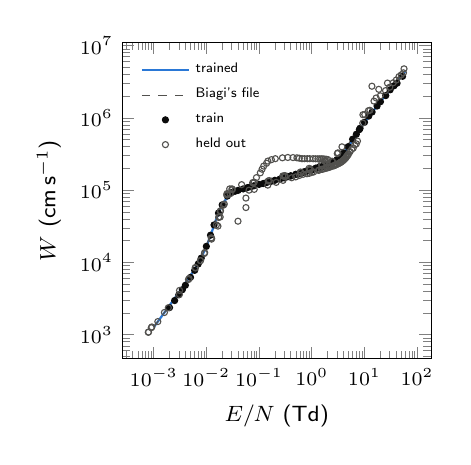
\begin{tikzpicture}
\begin{axis}[width=5.5cm, height=5.6cm, xmode=log, ymode=log,
  xlabel={$E/N$ (Td)}, ylabel={$W$ (cm\,s$^{-1}$)},
  tick label style={font=\scriptsize}, label style={font=\footnotesize},
  legend style={font=\tiny, draw=none, fill=none, at={(0.03,0.97)},
  anchor=north west}, legend cell align=left]
\plotcoords{cE, thick}{\wgSwWtr}
\addlegendentry{trained}
\plotcoords{ink2, dashed}{\wgSwWbi}
\addlegendentry{Biagi's file}
\plotcoords{only marks, mark=*, mark size=1.1pt, ink}{\wgSwWTdata}
\addlegendentry{train}
\plotcoords{only marks, mark=o, mark size=1.1pt, ink2}{\wgSwWHdata}
\addlegendentry{held out}
\end{axis}
\end{tikzpicture}\hfill
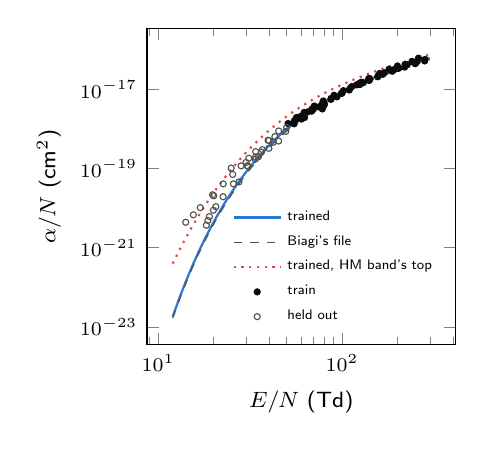
\begin{tikzpicture}
\begin{axis}[width=5.5cm, height=5.6cm, xmode=log, ymode=log,
  xlabel={$E/N$ (Td)}, ylabel={$\alpha/N$ (cm$^2$)},
  tick label style={font=\scriptsize}, label style={font=\footnotesize},
  legend style={font=\tiny, draw=none, fill=none, at={(0.97,0.03)},
  anchor=south east}, legend cell align=left]
\plotcoords{cE, thick}{\wgSwAtr}
\addlegendentry{trained}
\plotcoords{ink2, dashed}{\wgSwAbi}
\addlegendentry{Biagi's file}
\plotcoords{cH, dotted, thick}{\wgSwAHM}
\addlegendentry{trained, HM band's top}
\plotcoords{only marks, mark=*, mark size=1.1pt, ink}{\wgSwATdata}
\addlegendentry{train}
\plotcoords{only marks, mark=o, mark size=1.1pt, ink2}{\wgSwAHdata}
\addlegendentry{held out}
\end{axis}
\end{tikzpicture}\hfill
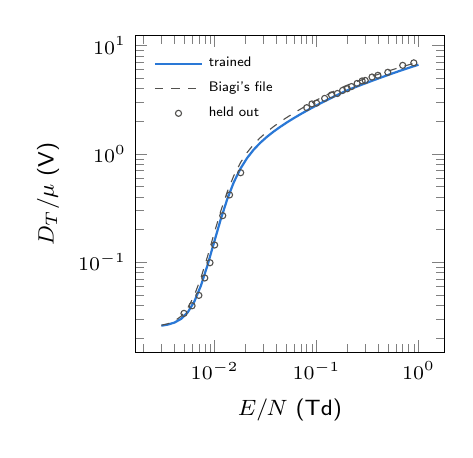
\begin{tikzpicture}
\begin{axis}[width=5.5cm, height=5.6cm, xmode=log, ymode=log,
  xlabel={$E/N$ (Td)}, ylabel={$D_T/\mu$ (V)},
  tick label style={font=\scriptsize}, label style={font=\footnotesize},
  legend style={font=\tiny, draw=none, fill=none, at={(0.03,0.97)},
  anchor=north west}, legend cell align=left]
\plotcoords{cE, thick}{\wgSwDtr}
\addlegendentry{trained}
\plotcoords{ink2, dashed}{\wgSwDbi}
\addlegendentry{Biagi's file}
\plotcoords{only marks, mark=o, mark size=1.1pt, ink2}{\wgSwDHdata}
\addlegendentry{held out}
\end{axis}
\end{tikzpicture}
\caption{Krypton's drift velocity (left), first Townsend coefficient
(middle) and characteristic energy (right) at 300\unit{K}, as the
experiments measure them: the trained cross sections (solid), Biagi's
file as published (dashed), and the measurements of
Table~\ref{tab:swdata}, filled where they train and open where they are
held out (the validation sets among them). Middle: the dotted curve is
the trained set with every excitation of the
levels at or above \Krtp's energy ionizing associatively (the
Hornbeck--Molnar band's top).}
\label{fig:swarm}
\end{figure}

\textbf{The scores.}
\begin{itemize}
\item \textbf{The train sets.} The drift velocity of Hunter et
al.~\cite{hunter88}, the most precise below 3\unit{Td}, moves from
$\chi^2$ \wg{sw.w_hunter88.bi.chi} to \wg{sw.w_hunter88.tr.chi} per
point, Nakamura's~\cite{nakamura90} from \wg{sw.w_nakamura90.bi.chi} to
\wg{sw.w_nakamura90.tr.chi} (mean \wg{sw.w_nakamura90.bi.mean} to
\wg{sw.w_nakamura90.tr.mean}\,\%). The ionization coefficients of
Jacques et al.~\cite{jacques86} and Kruithof~\cite{kruithof40}, which lay
\wg{sw.a_jacques86.bi.mean} and \wg{sw.a_kruithof40.bi.mean}\,\% from
the model, now lie \wg{sw.a_jacques86.tr.mean} and
\wg{sw.a_kruithof40.tr.mean}\,\%; Bhattacharya's~\cite{bhattacharya79},
which Biagi's file matched (\wg{sw.a_bhatta79.bi.mean}\,\%), now lies
\wg{sw.a_bhatta79.tr.mean}\,\%. Every train set ends within the
consistency threshold.
\item \textbf{The held-out drift velocities} are the sets the check
dropped. The training moves \wg{sw.wh.better} of the \wg{sw.wh.sets}
closer to the model, the two at 195\unit{K} among them, which took part
in choosing which factors train. Three move further: Pack et al.\ 1992
at 300\unit{K}~\cite{pack92} ($\chi^2$ \wg{sw.w_pack92.bi.chi} to
\wg{sw.w_pack92.tr.chi} per point), Dall'Armi et al.'s~\cite{dallarmi92}
(\wg{sw.w_dallarmi92.bi.chi} to \wg{sw.w_dallarmi92.tr.chi}) and
Kucukarpaci and Lucas's~\cite{kucukarpaci81} (\wg{sw.w_kucuk81.bi.chi}
to \wg{sw.w_kucuk81.tr.chi}, \wg{sw.w_kucuk81.tr.mean}\,\% from the
model on average). Pack et al.'s 1992 set scatters by up to
\wg{pack92.jump}\,\% against the model between points within 5\,\% of
each other in $E/N$; Bowe's~\cite{bowe60} lie
\wg{sw.w_bowe60.tr.mean}\,\% from the model, and English and
Hanna's~\cite{english53} \wg{sw.w_english53.tr.mean}\,\%.
\item \textbf{The characteristic energy} of Koizumi et
al.~\cite{koizumi86}, held out, probes the momentum transfer near the
Ramsauer minimum, which the drift velocities pin least: rms
\wg{sw.dtk.bi.rms}\,\% on Biagi's file and \wg{sw.dtk.tr.rms}\,\% on the
trained set. It chose which factors train, so it validates the training
rather than tests it.
\item \textbf{Below 50\unit{Td}}, held out by rule, the mean error moves
from \wg{sw.alow.bi.mean} to \wg{sw.alow.tr.mean}\,\%: Heylen's
from \wg{sw.a_heylen71_low.bi.mean} to \wg{sw.a_heylen71_low.tr.mean}\,\%,
Specht et al.'s direct coefficient~\cite{specht80} from
\wg{sw.a_specht80_direct.bi.mean} to
\wg{sw.a_specht80_direct.tr.mean}\,\%, Kruithof's from
\wg{sw.a_kruithof40_low.bi.mean} to \wg{sw.a_kruithof40_low.tr.mean}\,\%.
\end{itemize}

\textbf{Why the low field stays out.} At 30\unit{Td} the electrons excite
krypton \wg{low.exc_ion} times for every ionization, so anything that
ionizes an excited atom, or frees an electron at a surface with its
light, can dominate the measured current. Specht et al.\ found the
coefficient anomalously large at low field and attributed it to
photoelectron emission at the surfaces by radiating metastables, which
they say also explains why earlier measurements disagreed with transport
calculations; their direct coefficient leaves that contribution
out~\cite{specht80}. Bordage et al.\ found every published krypton set
below the low-field data and ascribe it to Penning ionization of
impurities~\cite{bordage13}. And the \wg{sw.low.sets} datasets part by up
to \x{\wg{sw.low.part}} from one another where they overlap. Training on
them would fit the cross sections to the purity and geometry of each
experiment. Pure krypton has one process there of its own, the
associative (Hornbeck--Molnar) ionization of atoms excited above
\wg{hm.eai}\unit{eV}~\cite{hornbeck51}. At the band's top it raises the
trained set's coefficient \x{\wg{hm.x14}} at 14\unit{Td}, \x{\wg{hm.x30}}
at 30\unit{Td} and \x{\wg{hm.x100}} at 100\unit{Td}, and puts the model
\wg{swhm.atr.mean}\,\% from the train sets on average, so a share that
large cannot hold where those are measured. No krypton measurement gives
the share, and it stays at 0 by default.

\textbf{What this means for the reference point.} The electrons sit at
\wg{ref.kin.en.lo} to \wg{ref.kin.en.hi}\unit{Td}. There direct
ionization makes \wm{ion.C2}\,\% of the ions and Penning ionization the
rest, so the low-field coefficient does not reach the answer. The
excitation rates do, and the training moves them: on Biagi's file as
published v0\_4 gives \wg{chg.kin.bi}\,\% at the reference point, and on
the trained set \wg{ref.kin.147}\,\% (\wg{chg.kin.bi.dev}\,\%); the
posterior of the factors spreads it by $\pm$\wg{unc.kin.xs.sd} points
(Section~\ref{sec:accuracy}).

\section{The electroluminescence yield}
\label{sec:el}

Mano et al.\ measured the secondary scintillation of pure krypton at
1.1\unit{bar} and room temperature: the photons an electron drifting in a
uniform field makes per centimetre, over the gas density~\cite{mano22}.
Below the field at which the electrons ionize, every photon comes from an
excitation, so the yield measures the excitation cross sections in the
swarm regime, where no electron meets another and no excited atom meets
an electron. Their fit, $Y/N = \wg{el.mano.a}\,E/N - \wg{el.mano.b}$ in
$10^{-17}$ photons per electron per atom per cm$^{-2}$ ($E/N$ in Td),
holds from its intercept at \wg{el.mano.thr}\unit{Td} to
\wg{el.mano.top}\unit{Td}. Nothing in v0\_4 or in its training saw it.

v0\_4's swarm (Section~\ref{sec:swarm}) gives the excitations per
electron and per centimetre of drift, $\sum k_\mathrm{exc}/W$, level by
level. Each excitation is then weighted by the photons the model's own
network makes of it at 1.1\unit{bar} and 296\unit{K}: a dilute seed of
each 5s level and of the 5p rung, with no drive and no electrons to speak
of, run to the end of its cascade. At the bands' defaults every seed ends
as one 147-nm photon (\wg{el.ph.1s5.default} per \lv{5} atom,
\wg{el.ph.1s4.default} per \lv{4} atom, \wg{el.ph.5p.default} per 5p
atom); with \Krts{} + Kr at its band's top, \wg{el.ph.5p.quench} per 5p
atom.

\begin{table}[H]
\centering\footnotesize
\begin{tabular}{@{}rrrrrr@{}}
\toprule
 & \multicolumn{2}{c}{$Y/N$ ($10^{-17}\unit{cm^2}$)} & \multicolumn{2}{c}{model over fit} & \\
\cmidrule(lr){2-3}\cmidrule(lr){4-5}
$E/N$ (Td) & Mano et al.'s fit & model & bands' defaults & \Krts{} + Kr at its top & 5s share (\%)\\
\midrule
\wgEl
\bottomrule
\end{tabular}
\caption{The electroluminescence yield of pure krypton: Mano et al.'s
fit~\cite{mano22} and v0\_4's swarm at 296\unit{K}, each excitation
weighted by its photons from the network's cascade at 1.1\unit{bar}; the
5s share is the excitations into the four 5s levels.}
\label{tab:el}
\end{table}

From 6 to 13.5\unit{Td} the model lies at \wg{el.lo} to \wg{el.hi} of the
fit (\wg{el.rms}\,\% rms), and with the excimer's quenching at its band's
top at \wg{el.q.lo} to \wg{el.q.hi}. Toward the fit's intercept it falls
below it (\wg{el.5} at 5\unit{Td}, \wg{el.4} at 4): there the fit's yield
is \wg{el.frac5} and \wg{el.frac4} of its value at 13.5\unit{Td}, and a
straight line's intercept is the least constrained part of a fit to a
yield that bends into its threshold. Nearly every excitation below 14\unit{Td} is a 5s
level's, so the score tests the four 5s cross sections and the trained
5s factor (\x{\wg{fac.x_1s}}) at the swarm's mean energies of
\wg{el.mean.lo} to \wg{el.mean.hi}\unit{eV}, and the
excitation-to-photon chain at a density where nothing competes with the
light.

\section{Under an electron beam}
\label{sec:beam}

Three measurements bear on the chain from excitation to the 147-nm
photon. They were made under electron beams, so for them v0\_4 runs under
a beam drive. The drive is a fixture of this note, not part of the model.
It deposits the given power as ion pairs, 5s and 5p atoms and secondary
electrons in the proportions of a fast electron's degradation in pure
krypton. That degradation is the Fowler--Spencer--Fano recursion on the
same cross sections as the model, level by level, from
\wg{beam.e0}\unit{eV}: an excitation continues the electron at $E-I$, and
an ionization shares $E-I$ equally between the two electrons. Per ion
pair it gives:
\begin{itemize}
\item $W=\wg{beam.W}\unit{eV}$;
\item \wg{beam.pp} \Krpp, from the levels above the 5s manifold;
\item \wg{beam.s} 5s atoms: \wg{beam.s.1s5} \lv{5}, \wg{beam.s.1s4}
\lv{4}, \wg{beam.s.1s3} \lv{3} and \wg{beam.s.1s2} \lv{2}, the two
resonance levels most, as a fast electron's dipole excitation favours
them (v0\_3 put the four into one \Krs);
\item \wg{beam.cascade}\unit{eV} of heat, the higher levels' excess over
the 5p rung's energy;
\item \wg{beam.eps}\unit{eV} of sub-excitation secondaries, which the
kinetic equation injects with a flat spectrum up to \wm{E.S}\unit{eV}.
\end{itemize}
That is one excitation or ion per \wg{beam.ws}\unit{eV}.

\textbf{The partition.} Saito et al.~\cite{saito03} measured scintillation
photons and electrons together under 5.49-MeV alpha particles in 1 to
10\unit{atm} of krypton. They found \wg{saito.nex} excited atoms per ion
pair, and $W_s=\wg{saito.ws}\unit{eV}$, the energy per photon when every
pair recombines. They also confirmed that each recombination gives one
photon. On the trained cross sections the drive's \wg{beam.ws}\unit{eV}
per excitation or ion is \wg{beam.ws.dev}\,\% from their $W_s$, its
excitations per pair (\wg{beam.nex}) differ from theirs by
\wg{beam.nex.dev}\,\%, and its $W$ differs by \wg{beam.W.dev}\,\% from
the \wg{saito.W}\unit{eV} their two numbers imply. On Biagi's file as
published the same degradation gives $W=\wg{beam.W.v02}\unit{eV}$
(\wg{beam.W.dev.v02}\,\%) and \wg{beam.nex.v02} excitations per pair
(\wg{beam.nex.dev.v02}\,\%): the swarm data's smaller excitation moves
both toward the measurement, which neither the training nor the choice
of its factors saw. One photon of \wg{hv147}\unit{eV} per
\wg{saito.ws}\unit{eV} is an efficiency of \wg{saito.ideal}. The model's
ceiling, one photon per excitation and per ion of the drive, is
\wg{beam.ceil}.

\textbf{Low pump.} Morozov et al.~\cite{morozov08} measured the power a
continuous 8 to 15-keV beam deposits in the gas against the VUV power
emitted into $4\pi$. For krypton they found \wg{moz.meas} $\pm$
\wg{moz.err}, flat from 500 to 1400\unit{hPa} and over a tenfold range of
beam power. At \wg{moz.hpa}\unit{hPa}, \wg{moz.w.lo} and
\wg{moz.w.hi}\unit{W\,cm^{-3}} for \wg{beam.pulse}\unit{\mu s} with the
light counted for \wg{beam.tail.lo}\unit{\mu s} after, v0\_4 gives
\wg{moz.30.kin} and \wg{moz.300.kin} (Table~\ref{tab:beam}). The error is
\wg{moz.kin.dev}\,\%, \wg{moz.kin.sig} of the measurement's standard
errors (v0\_3: \wg{moz.kin.dev.v03}\,\%). At this pump nothing competes
with the light: \wg{moz.300.kin.G2} Penning ionizations per pair, every
ion recombined (\wg{moz.300.kin.rec} per pair), \wg{moz.300.kin.redis}
excimers redissociated per pair, and every \Krts{} radiating. So v0\_4
sits at its ceiling, which Saito et al.'s measurement supports. Morozov
et al.\ compare their value with calculated maxima of 0.46 and 0.52 for
krypton. The \wg{moz.short}\,\% between their value and Saito et al.'s
one photon per excitation and per ion (\wg{saito.ideal}) is not explained
in v0\_4.

\textbf{High pump.} Eckstrom et al.~\cite{eckstrom88} report the
fluorescence efficiency of \Krts{} near their theoretical limit of about
46\,\%. They found it under a low-current, long-pulse beam at modest
pressures, for pump rates up to $3\times10^5\unit{W\,cm^{-3}}$. The
abstract does not give the pressure of each point. At that pump rate
(1\unit{\mu s}, the light counted for \wg{beam.tail.hi}\unit{\mu s})
v0\_4 gives:
\begin{itemize}
\item \wg{eck.0.5.kin} at 0.5\unit{atm}, \wg{eck.1.kin} at 1\unit{atm}
and \wg{eck.2.kin} at 2\unit{atm}, that is \wg{eck.0.5.kin.loss},
\wg{eck.1.kin.loss} and \wg{eck.2.kin.loss}\,\% below its ceiling of
\wg{beam.ceil} (v0\_3: \wg{eck.0.5.kin.v03}, \wg{eck.1.kin.v03} and
\wg{eck.2.kin.v03});
\item at 1\unit{atm}, Penning ionization of the 5s levels on one another
costs \wg{eck.1.kin.G2} photons per pair, because the excimer forms too
slowly to outrun it entirely;
\item at 1\unit{atm} with \Krs{} + \Krs{} at its band's low end,
\wg{eck_pen.1.kin} (\wg{eck_pen.1.kin.loss}\,\% below the ceiling), and
with the \lv{5} formation at its band's top, \wg{eck_form.1.kin}
(\wg{eck_form.1.kin.loss}\,\%).
\end{itemize}
Their limit assumes other numbers than v0\_4's ceiling, so what the
report tests is the loss: little at high pump. At 1\unit{atm} v0\_4 now
meets it (\wg{eck.kin.dev}\,\%; v0\_3: \wg{eck.kin.dev.v03}\,\%),
losing \wg{eck.1.kin.loss}\,\% below its ceiling where v0\_3 lost more:
its faster formation, out of \lv{4} above all, outruns the Penning loss.
At 0.5\unit{atm} the gas heats to \wg{eck.0.5.kin.tg}\unit{K} and the
excimer redissociates (\wg{eck.0.5.kin.redis} per pair), and at
2\unit{atm} v0\_4 loses \wg{eck.2.kin.loss}\,\%. The report gives no
pressure for its points, so it no longer leans on the defaults.

\begin{table}[H]
\centering\footnotesize
\resizebox{\linewidth}{!}{%
\begin{tabular}{@{}llrrrrrrr@{}}
\toprule
run & measured & kinetic & two-temperature & v0\_3, kinetic & Penning per pair & photons per pair & $T_e$ (eV) & $T_g$ end (K)\\
\midrule
\wg{moz.w.lo}\unit{W\,cm^{-3}}, \wg{moz.hpa}\unit{hPa} & \wg{moz.meas} $\pm$ \wg{moz.err} & \wg{moz.30.kin} & \wg{moz.30.2t} & & \wg{moz.30.kin.G2} & \wg{moz.30.kin.ph} & \wg{moz.30.kin.te} & \wg{moz.30.kin.tg}\\
\wg{moz.w.hi}\unit{W\,cm^{-3}}, \wg{moz.hpa}\unit{hPa} & \wg{moz.meas} $\pm$ \wg{moz.err} & \wg{moz.300.kin} & \wg{moz.300.2t} & \wg{moz.kin.v03} & \wg{moz.300.kin.G2} & \wg{moz.300.kin.ph} & \wg{moz.300.kin.te} & \wg{moz.300.kin.tg}\\
$3\times10^5\unit{W\,cm^{-3}}$, 0.5\unit{atm} & near \wg{eck.meas} & \wg{eck.0.5.kin} & \wg{eck.0.5.2t} & \wg{eck.0.5.kin.v03} & \wg{eck.0.5.kin.G2} & \wg{eck.0.5.kin.ph} & \wg{eck.0.5.kin.te} & \wg{eck.0.5.kin.tg}\\
$3\times10^5\unit{W\,cm^{-3}}$, 1\unit{atm} & near \wg{eck.meas} & \wg{eck.1.kin} & \wg{eck.1.2t} & \wg{eck.1.kin.v03} & \wg{eck.1.kin.G2} & \wg{eck.1.kin.ph} & \wg{eck.1.kin.te} & \wg{eck.1.kin.tg}\\
$3\times10^5\unit{W\,cm^{-3}}$, 2\unit{atm} & near \wg{eck.meas} & \wg{eck.2.kin} & \wg{eck.2.2t} & \wg{eck.2.kin.v03} & \wg{eck.2.kin.G2} & \wg{eck.2.kin.ph} & \wg{eck.2.kin.te} & \wg{eck.2.kin.tg}\\
\quad 1\unit{atm}, \Krs{} + \Krs{} $\wm{bd.kr_pen.lo}$ & & \wg{eck_pen.1.kin} & \wg{eck_pen.1.2t} & & \wg{eck_pen.1.kin.G2} & \wg{eck_pen.1.kin.ph} & \wg{eck_pen.1.kin.te} & \wg{eck_pen.1.kin.tg}\\
\quad 1\unit{atm}, \lv{5} + 2Kr $\wm{bd.kr2_form.hi}$ & & \wg{eck_form.1.kin} & \wg{eck_form.1.2t} & & \wg{eck_form.1.kin.G2} & \wg{eck_form.1.kin.ph} & \wg{eck_form.1.kin.te} & \wg{eck_form.1.kin.tg}\\
\bottomrule
\end{tabular}}
\caption{v0\_4 under the beam drive: the VUV efficiency (147-nm energy
over the deposited energy) on both closures and v0\_3's on the kinetic
EEDF, and on the kinetic EEDF the Penning ionizations and 147-nm photons
per ion pair, the pulse's mean $T_e$ and the final gas temperature. The
ceiling, one photon per excitation and per ion, is \wg{beam.php} photons
per pair, an efficiency of \wg{beam.ceil}; Saito et al.'s ideal is
\wg{saito.ideal}.}
\label{tab:beam}
\end{table}

\section{The energy ladder}

Figure~\ref{fig:ladder} draws v0\_4's levels at their formation energies
and the rows that move energy between them.

\begin{figure}[H]
\centering
\begin{tikzpicture}[x=1cm, y=0.6cm, font=\scriptsize,
  arr/.style={-{Stealth[length=4pt]}},
  heat/.style={cH, decorate, decoration={snake, amplitude=1pt,
    segment length=4pt, post length=4pt}, -{Stealth[length=4pt]}}]
\newcommand\lev[4]{\draw[line width=1.1pt, #4] (#1,#3) -- (#2,#3);}
% atoms: the four 5s levels, the 5p rung, the ion
\lev{0}{4.6}{0}{ink}
\lev{0}{1.15}{\wg{lad.1s5}}{cX}
\lev{1.15}{2.3}{\wg{lad.1s4}}{cX}
\lev{2.3}{3.45}{\wg{lad.1s3}}{cX}
\lev{3.45}{4.6}{\wg{lad.1s2}}{cX}
\lev{0}{4.6}{\wg{lad.P}}{cP}
\lev{0}{4.6}{\wg{lad.I}}{cI}
\node[left] at (0,0) {Kr, 0};
\node[left, align=right] at (0,\wg{lad.1s5}+0.2) {\Krs{} (5s): \lv{5}
  \wg{lad.1s5},\\ \lv{4} \wg{lad.1s4}, \lv{3} \wg{lad.1s3}, \lv{2}
  \wg{lad.1s2}};
\node[left] at (0,\wg{lad.P}) {\Krpp{} (5p) \wg{lad.P}};
\node[left] at (0,\wg{lad.I}) {\Krp{} \wg{lad.I}};
% molecules
\lev{7.4}{9.6}{0}{ink}
\lev{7.4}{9.6}{\wg{lad.X2}}{cV}
\lev{7.4}{9.6}{\wg{lad.I2}}{cI}
\draw[ink2, dashed] (7.4,\wg{lad.low}) -- (9.6,\wg{lad.low});
\node[right] at (9.6,0) {2Kr, 0};
\node[right, align=left] at (9.6,\wg{lad.X2}) {\Krts{} \wg{lad.X2}\\
  (0$_u^+$ \wg{lad.F2})};
\node[right] at (9.6,\wg{lad.I2}) {\Krtp{} \wg{lad.I2}};
\node[right, ink2] at (9.6,\wg{lad.low}) {repulsive 2Kr, \wg{lad.low}};
% electron impact from the ground state
\draw[cE, arr] (0.4,0) -- (0.4,\wg{lad.1s5}) node[pos=0.45, right] {G1};
\draw[cE, arr] (1.0,0) -- (1.0,\wg{lad.P}) node[pos=0.45, right] {C1};
\draw[cE, arr] (1.6,0) -- (1.6,\wg{lad.I}) node[pos=0.45, right] {C2};
% Penning ionization of the 5s levels on one another
\draw[ink2, densely dashed, arr] (2.3,\wg{lad.1s3}) -- (2.3,\wg{lad.I})
  node[pos=0.75, right] {G2};
% the 5s <-> 5p cycle, its relaxation and its light
\draw[cE, arr] (3.0,\wg{lad.1s3}) -- (3.0,\wg{lad.P});
\draw[cE, arr] (3.25,\wg{lad.P}) -- (3.25,\wg{lad.1s3});
\draw[heat] (3.75,\wg{lad.P}) -- (3.75,\wg{lad.1s2});
\draw[cP, arr] (4.25,\wg{lad.P}) -- (4.25,\wg{lad.1s2});
\node[ink, anchor=north west, align=left, inner sep=1pt] at (2.75,9.0)
  {\textcolor{cE}{K76, K76r,}\\ \textcolor{cH}{KPS},
  \textcolor{cP}{PRAD}\\ \textcolor{ink2}{each 5s level's}};
% to the excimer, its reverse and its light
\draw[cX, arr] (4.6,\wg{lad.1s5}) -- (7.4,\wg{lad.X2});
\draw[cX, arr, densely dotted] (7.4,\wg{lad.X2}+0.45) -- (4.6,\wg{lad.1s5}+0.45);
\node[cX, anchor=north west, align=left] at (4.7,8.65) {AK8, \lv{5}:
  \wg{lad.ak8} to heat;\\ AK8r back, dotted};
\draw[cV, arr] (8.1,\wg{lad.X2}) -- (8.1,\wg{lad.low})
  node[pos=0.5, right, cV] {KR2\_RAD, $h\nu$ \wg{lad.hv}};
\draw[heat] (8.1,\wg{lad.low}) -- (8.1,0);
% the ions
\draw[cI, arr] (4.6,\wg{lad.I}) -- (7.4,\wg{lad.I2});
\node[cI, anchor=south west] at (7.45,13.25) {K15 (K15r back), \wg{lad.k15} to heat};
\draw[cI, arr] (7.4,\wg{lad.I2}) -- (4.6,\wg{lad.P});
\node[cI, anchor=north west] at (7.45,12.4) {R11p, \wg{lad.r11} to heat};
\end{tikzpicture}
\caption{v0\_4's energy ladder in eV above ground-state krypton at rest.
A bar is a species at its formation energy; the four 5s levels are
drawn side by side. Blue arrows are electron impact, which takes its
energy from the electron gas; K76r, the 5p \ra 5s arrow beside K76,
returns it. The dashed G2 is the Penning ionization of the 5s levels on
one another, which gives the electron \wg{lad.pen}\unit{eV} for two
\lv{5} atoms. A red squiggle is heat: KPS relaxes the 5p rung on
krypton, and PRAD radiates its gap to each level, \wg{lad.gap.1s2} to
\wg{lad.gap.1s5}\unit{eV}, in the near infrared. The excimer forms out
of each 5s level, its well and the level's excess to heat, redissociates
by detailed balance (AK8r), and radiates onto the repulsive ground state,
which falls apart and heats the gas. The 5s levels exchange population on
krypton (MIX, not drawn). C1's levels, \wg{lad.c1lo} to
\wg{lad.c1hi}\unit{eV}, cascade to the 5p rung, each heating the gas with
its excess. HM, the Hornbeck--Molnar ionization of the levels above
\Krtp's energy, and the resonance lines of \lv{4} and \lv{2} are bands at
0 and not drawn.}
\label{fig:ladder}
\end{figure}

\section{Where v0\_4 is not yet reliable}

\begin{itemize}
\item \textbf{The excimer's formation.} Its rates still decide much of
the answer. The \lv{5} rate's measurements spread by a factor of
\wg{form.ratio}; the \lv{4} rate is one measurement~\cite{marchal18},
which Audouard et al.'s formation-time ratio puts three times
lower~\cite{audouard88} and Janssens et al.'s quasiclassical calculation
1.5 times higher~\cite{janssens87}; the \lv{3} rate is a proxy, the
value of Kholin et al.'s measurement~\cite{kholin15} not being in a
source in hand. The temperature law is measured over 200 to
400\unit{K}~\cite{wieme81} (v0\_1 to v0\_3 said 451\unit{K}, the range of
a conversion), and the reference point ends at \wg{ref.kin.tg}\unit{K}.
\item \textbf{The field-driven regime is unscored.} No pure-krypton
measurement in hand tests the 5s $\leftrightarrow$ 5p cycle under a field.
Its cross sections are measured to $\pm$\wg{jung.unc.1s5} to
\wg{jung.unc.1s3}\,\% out of the two metastables; those of the two $J=1$
levels are not measured and take their metastable's (band
\texttt{k\_5s5p\_j1}). The ledger books the 5p rung at the 2p$_{10}$
energy, so an electron that pumps \lv{3} or \lv{2} pays that level's gap
to it, \wg{lad.gap.1s3} or \wg{lad.gap.1s2}\unit{eV}, where the
core-preserving transitions out of those levels reach the 2p$_1$ to
2p$_4$ levels, \wg{lad.core.lo} to \wg{lad.core.hi}\unit{eV} up, and their
near-infrared lines carry the same gap.
\item \textbf{The redissociation} rests on the excimer's well, whose
measurements give 0.62 to 0.709\unit{eV} (its band), and on a rotational
constant from an estimated bond length, 2.6\,\AA, the ion's, which enters
as $1/r_e^2$; the ion's vibrational quantum is taken as the excimer's. At
the reference point \wg{ref.kin.redis}\,\% of the excimers formed
redissociate; above \wg{keq.half.K}\unit{K} at the fill's density most
would.
\item \textbf{Hot gas.} The 5p rung's relaxation by krypton carries no
reverse, so the gas can de-excite the rung but not excite the 5s levels to
it. By detailed balance that reverse out of \lv{2} would match \lv{4}'s
excimer formation at the fill's density at \wg{kpsr.T}\unit{K}; below it,
and at the reference point, it is negligible. The scan's 0.1 and
0.25\unit{atm} columns reach several thousand kelvin, where it is not,
nor are the measured ranges of the formation and the recombination.
\item \textbf{The excimer's two states.} The fast 0$_u^+$ state takes no
share by default: its measured share is above $6\times10^{19}\unit{cm^{-3}}$
and appears from $1.5\times10^{19}$~\cite{audouard88}, so at 1\unit{atm}
it lies between 0 and the band's top. Quenching by krypton is 0 by
default, against one measurement of a pressure-dependent decay at
984\unit{nm}~\cite{firestone88} that may be a transfer between radiating
states rather than a loss. No rate mixes the two states, by krypton or
by electrons.
\item \textbf{The two-temperature closure} reads a tail table built from
states without excited atoms. The run's 5s and 5p populations keep its
tail hotter than the table's (Section~\ref{sec:twot}), and its Maxwellian
below the break errs the other way; the closure is
\wg{tail.pt.1.300.f}\,\% from the kinetic EEDF at the reference point and
within \wg{tail.worst.f}\,\% at the scan's corners. The default closure
does not use it.
\item \textbf{The trained cross sections} rest on errors the swarm data
do not print (class values here) and on the consistency check's threshold
(at 4 rather than 3, \wg{cons.at4.n} more sets train and the momentum
transfer at 6\unit{eV} moves to \x{\wg{cons.at4.m6}}). The data barely
pin the 5p excitation. Which factors train was chosen on held-out data
(Table~\ref{tab:var}), so those sets validate the training rather than
test it. Their posterior is propagated into the answer
($\pm$\wg{unc.kin.xs.sd} points).
\item \textbf{The rows with no measurement.} \Krts{} + \Krts{} and the
stepwise ionizations of the 5s levels and of \Krpp{} are 0 by default
(Table~\ref{tab:unc}). At its band's top \Krts{} + \Krts{} cuts the
147-nm share by \wg{unc.cut.kr2_pen}\,\%, the stepwise ionization of the
5s levels by \wg{unc.cut.kstep_s}\,\% and that of \Krpp{} by
\wg{unc.cut.kstep_p}\,\%. The $J=1$ levels' 5s \ra 5p cross sections
are proxies, and their scale is the uncertainty's largest term.
\item \textbf{\Krs{} + \Krs.} Its $\wm{k.G2}\cm{3}$ is a 1974
measurement~\cite{leichner74} as Kannari et al.\ print it~\cite{kannari85},
taken for every pair of levels.
\item \textbf{The e-beam efficiency at low pump} is off Morozov et
al.'s by \wg{moz.kin.dev}\,\%, and v0\_4 holds no process that would
explain the difference.
\item \textbf{The ionization coefficient below 50\unit{Td}} lies
\wg{sw.alow.tr.mean}\,\% from the measurements on average, which part by
up to \x{\wg{sw.low.part}} from one another; every published
cross-section set falls below them~\cite{bordage13}. It is held out of the
training by rule, and it does not reach the reference point, where
Penning ionization makes the ions.
\item \textbf{The Hornbeck--Molnar share} of the levels above
\wg{hm.eai}\unit{eV} is not measured for krypton and is 0 by default. At
its top it puts the model \wg{swhm.atr.mean}\,\% from the train sets and
moves the reference point by \wg{unc.hm.cut}\,\%.
\item \textbf{Processes v0\_4 does not carry}, each needing a measured
rate before it can enter:
\begin{itemize}
\item Kr$_3^+$ and its recombination;
\item electron collisions with \Krts{}: ionization, quenching and the
mixing of its two states;
\item Penning ionization between \Krs{} and \Krts, and of \Krpp;
\item the electrons' transfers between the 5s levels, and their
superelastic return of the 5s levels to the ground state, which Blagoev
et al.\ measured for thermal electrons in an afterglow~\cite{blagoev84}
but which v0\_4's kinetic EEDF would need as cross sections.
\end{itemize}
Three-body recombination \Krp{} + \el{} + \el~\cite{mansbach69} is not
carried either: at 1\unit{atm} \Krp{} converts to \Krtp{} in
\wg{k15.ns}\unit{ns}.
\end{itemize}

\textbf{How the numbers were made.} Every number in this note is computed
from the model when the note is built. None is typed by hand except the
measurements, which carry their sources, and the training's record, which
the model carries beside its cross sections and the training wrote. The
runs are cached under a hash of the model's code, so a change to the
model reruns them all (code \texttt{\wg{md5}}). The kinetic runs take
about \wg{ref.kin.min} minutes each; the two-temperature runs take
seconds.

\appendix
\section{Reaction rates}
\label{app:rates}

The rows of v0\_4 with the values they run with and their sources, a
\texttt{<level>} row once per 5s level. Electron-impact rows use their
cross sections over the kinetic EEDF (or the two-temperature closure). A
band gives its default and its two ends.

\begin{table}[H]
\centering\scriptsize
\renewcommand{\arraystretch}{1.1}
\begin{tabularx}{\linewidth}{@{}>{\raggedright\arraybackslash}p{1.8cm}>{\raggedright\arraybackslash}p{3.3cm}>{\raggedright\arraybackslash}p{5.15cm}>{\raggedright\arraybackslash}X@{}}
\toprule
row & reaction & value & source\\
\midrule
G1\_<level> & \el{} + Kr \ra \el{} + \Krs(level) & each 5s level at its threshold, \wm{E.1s5} to \wg{lad.s2}\unit{eV}, its own species & Biagi, Magboltz 8.97~\cite{biagi99,pancheshnyi12,carbone21}, \x{\wg{fac.x_1s}} (trained, Table~\ref{tab:fac})\\
C1 & \el{} + Kr \ra \el{} + \Krpp & the 5p, 4d, 6s and higher levels, \wg{lad.c1lo} to \wg{lad.c1hi}\unit{eV}, \x{\wg{fac.x_2p}} (5p) and \x{\wg{fac.x_hi}} (higher) trained; the excess over \wm{E.PP} to heat & Biagi, Magboltz 8.97\\
HM & \el{} + Kr (+ Kr) \ra \Krtp{} + 2\el & the share of the excitations of the \wg{hm.levels} levels at or above \wg{hm.eai}\unit{eV}; band 0 (default) to 1 & no measurement for krypton; the process, Hornbeck and Molnar~\cite{hornbeck51}\\
C2 & \el{} + Kr \ra \Krp{} + 2\el & \wm{E.ion}\unit{eV} & Biagi, Magboltz 8.97\\
G6 & \el{} + Kr, elastic & the momentum transfer cross section, times the trained factor & Biagi, Magboltz 8.97\\
K76\_<level>, K76r & \el{} + \Krs(level) $\rightleftarrows$ \el{} + \Krpp & the measured cross sections out of \lv{5} and \lv{3}, the $J=1$ levels on their same-core metastable's; band \x{} \wm{bd.k_5s5p.lo} to \wm{bd.k_5s5p.hi}, and \x{} 0 to 1 on the $J=1$ levels; the reverse by detailed balance over each level's gap & Jung et al.~\cite{jung06,jung05}; Kannari's fit as a comparison~\cite{kannari85,jacob76}\\
KPS\_<level> & \Krpp{} + Kr \ra \Krs(level) + Kr & $\wm{k.KPS}\cm{3}$ in all, over the levels by $2J+1$ (band \texttt{kps\_5s}: 1, to all into \lv{5}); band $\wm{bd.kps_kr.lo}$ to the default & Gazeli et al.~\cite{gazeli21}, one level, products unresolved; the low end, the range Chang and Setser measured for argon's 4p levels~\cite{chang78}\\
PRAD\_<level> & \Krpp{} \ra \Krs(level) + $h\nu$, near IR & $\tau=\wg{tau5p}\unit{ns}$, the $2J+1$ mean of the ten 5p levels, branching by NIST's Einstein coefficients weighted by $2J+1$ & Dzier\.z\k{e}ga et al.~\cite{dzierzega00}; a TALIF lifetime of one level, 34.1\unit{ns}, as a cross-check~\cite{gazeli21rev}; NIST ASD~\cite{nistasd}\\
G2\_<a>\_<b> & \Krs(a) + \Krs(b) \ra \Krp{} + Kr + \el & $\wm{k.G2}\cm{3}$ for each pair (twice for two levels); band $\wm{bd.kr_pen.lo}$ to the default & Leichner and Ericson~\cite{leichner74} as Kannari et al.\ print it~\cite{kannari85}\\
AK8\_1s5 & \Krs(\lv{5}) + 2Kr \ra \Krts{} + Kr & $\wm{k.AK8}\cm{6}\times(T_g/300)^{\wm{tpow.AK8}}$; band $\wm{bd.kr2_form.lo}$ to $\wm{bd.kr2_form.hi}$ & Marchal et al.~\cite{marchal18}; Ueda et al.~\cite{ueda84}, Tracy and Oskam~\cite{tracy76}, Turner~\cite{turner67} and Smith and Turner~\cite{smith63} span the band; the law, Wieme and Lenaerts, 200 to 400\unit{K}~\cite{wieme81}\\
AK8\_1s4, AK8f & \Krs(\lv{4}) + 2Kr \ra \Krts{} + Kr & $\wm{k.AK8.1s4}\cm{6}$, the same law; band to a third of the \lv{5} rate; the share into the fast 0$_u^+$ state, band \wm{bd.kr2_fast.lo} to \wm{bd.kr2_fast.hi} & Marchal et al.~\cite{marchal18}; Audouard et al.~\cite{audouard88}\\
AK8\_1s3 & \Krs(\lv{3}) + 2Kr \ra \Krts{} + Kr & the \lv{5} rate as a proxy; band 0 to the \lv{4} rate & Kholin et al.\ measured it~\cite{kholin15}, the value not in a source in hand\\
AK8r\_<level> & \Krts{} + Kr \ra \Krs(level) + 2Kr & detailed balance on the excimer's well, $D_0$ \wm{bd.kr2_d0.def}\unit{eV}; band to \wm{bd.kr2_d0.lo}\unit{eV} & LaRocque et al.~\cite{larocque86}, Killeen and Eden~\cite{killeen86}\\
MIX & \Krs(\lv{4}) + Kr \ra \Krs(\lv{5}) + Kr, and \Krs(\lv{2}) + 2Kr \ra \Krs(\lv{4}) + 2Kr & $1.3\times10^{-13}\cm{3}$ at 295\unit{K} on $(T_g/295)^{-1.29}$ through Turner's 196-K point, and $0.2\times10^{-32}\cm{6}$; their reverses by detailed balance & Turner~\cite{turner67}; Audouard et al.~\cite{audouard91}\\
RES & \Krs(\lv{4}, \lv{2}) \ra Kr + $h\nu$, 123.6 and 116.5\unit{nm} & the escaping share; band 0 to $1.7\times10^5\unit{s^{-1}}$ & the pressure-independent term of Janssens et al.'s loss rate~\cite{janssens87}\\
KR2\_RAD & \Krts{} \ra 2Kr + $h\nu$, 147\unit{nm} & $\tau=\wm{tauRAD}\unit{ns}$, $h\nu=\wm{hv.RAD}\unit{eV}$ & Morikawa et al., 270 $\pm$ 5\unit{ns}~\cite{morikawa89}; 250 $\pm$ 20~\cite{salamero79}, 280 $\pm$ 30~\cite{quigley78}\\
KR2F\_RAD & \Krts(0$_u^+$) \ra 2Kr + $h\nu$ & $\tau=\wm{tauRADF}\unit{ns}$ & Morikawa et al.~\cite{morikawa89}\\
QKR2 & \Krts{} + Kr \ra 3Kr & 0; band to $\wm{bd.kr2_quench.hi}\cm{3}$ & Oka et al.~\cite{oka74}; Firestone and Selander~\cite{firestone88}\\
PEN\_KR2 & \Krts{} + \Krts{} \ra \Krtp{} + 2Kr + \el & 0; band to $\wm{bd.kr2_pen.hi}$ & no measurement; Kannari et al.'s value is the top~\cite{kannari85}\\
K15, K15r & \Krp{} + 2Kr $\rightleftarrows$ \Krtp{} + Kr & $\wm{k.K15}\cm{6}\times(T_g/300)^{\wm{tpow.K15}}$; the reverse by detailed balance on the ion's 1.149\unit{eV} & the mean of three measurements~\cite{bhattacharya70,grossl81,smith72}; the law, P\'erez-R\'ios and Greene~\cite{perezrios18}; Signorell et al.~\cite{signorell01}\\
R11p & \Krtp{} + \el{} \ra \Krpp{} + Kr & $\wm{k.R11p}\,(300\,\mathrm{K}/T_e)^{\wm{pow.R11p}}\cm{3}$, $\pm$10\,\%; a gas-temperature factor, band 0 to 1 & Shiu and Biondi~\cite{shiu77}; Mikus within 8\,\%~\cite{mikus78}; Cunningham and Hobson~\cite{cunningham72}\\
KSTEP\_S, KSTEP\_P & \el{} + \Krs(level), \Krpp{} \ra \Krp{} + 2\el & 0; bands to $\wm{bd.kstep_s.hi}\,T_e^{0.68}e^{-C/T_e}$ and $\wm{bd.kstep_p.hi}\,T_e^{0.62}e^{-2.53/T_e}\cm{3}$ & no measurement; Vriens' calculation~\cite{vriens65} as Kannari et al.\ print it~\cite{kannari85}\\
\bottomrule
\end{tabularx}
\caption{v0\_4's rows. Rates in cm$^3$\,s$^{-1}$ or cm$^6$\,s$^{-1}$, $T_e$
in eV; $C$ is 4.04\unit{eV} less the level's height above \lv{5}.
\Krtp{} lies \wg{lad.k15}\unit{eV} below \Krp{} + Kr~\cite{ng77}.}
\end{table}

\begin{thebibliography}{99}
\footnotesize
\setlength{\itemsep}{1pt}
\bibitem{biagi99} S.~F.~Biagi, Nucl.\ Instrum.\ Methods A 421, 234 (1999), doi:10.1016/S0168-9002(98)01233-9.
\bibitem{bordage13} M.~C.~Bordage, S.~F.~Biagi, L.~L.~Alves, K.~Bartschat, S.~Chowdhury, L.~C.~Pitchford, G.~J.~M.~Hagelaar, W.~L.~Morgan, V.~Puech and O.~Zatsarinny, J.\ Phys.\ D 46, 334003 (2013), doi:10.1088/0022-3727/46/33/334003.
\bibitem{dias23} T.~C.~Dias, A.~Tejero-del-Caz, L.~L.~Alves and V.~Guerra, Comput.\ Phys.\ Commun.\ 282, 108554 (2023), doi:10.1016/j.cpc.2022.108554.
\bibitem{hornbeck51} J.~A.~Hornbeck and J.~P.~Molnar, Phys.\ Rev.\ 84, 621 (1951), doi:10.1103/PhysRev.84.621.
\bibitem{jacques86} L.~Jacques, W.~Bruynooghe, R.~Boucique and W.~Wieme, J.\ Phys.\ D 19, 1731 (1986), doi:10.1088/0022-3727/19/9/017.
\bibitem{pancheshnyi12} S.~Pancheshnyi et al., Chem.\ Phys.\ 398, 148 (2012), doi:10.1016/j.chemphys.2011.04.020.
\bibitem{carbone21} E.~Carbone et al., Atoms 9, 16 (2021), doi:10.3390/atoms9010016.
\bibitem{hagelaar05} G.~J.~M.~Hagelaar and L.~C.~Pitchford, Plasma Sources Sci.\ Technol.\ 14, 722 (2005), doi:10.1088/0963-0252/14/4/011.
\bibitem{jung05} R.~O.~Jung, T.~E.~Stone, J.~B.~Boffard, L.~W.~Anderson and C.~C.~Lin, Phys.\ Rev.\ Lett.\ 94, 163202 (2005), doi:10.1103/PhysRevLett.94.163202.
\bibitem{jung06} R.~O.~Jung, T.~E.~Stone, J.~B.~Boffard, L.~W.~Anderson and C.~C.~Lin, Phys.\ Rev.\ A 73, 022722 (2006), doi:10.1103/PhysRevA.73.022722.
\bibitem{kannari85} F.~Kannari, M.~Obara and T.~Fujioka, J.\ Appl.\ Phys.\ 57, 4309 (1985), doi:10.1063/1.334590.
\bibitem{jacob76} J.~H.~Jacob and J.~A.~Mangano, Appl.\ Phys.\ Lett.\ 28, 724 (1976), doi:10.1063/1.88629.
\bibitem{vriens65} L.~Vriens, Physica 31, 385 (1965), doi:10.1016/0031-8914(65)90043-1.
\bibitem{gazeli21} K.~Gazeli et al., Phys.\ Plasmas 28, 043301 (2021), doi:10.1063/5.0041471.
\bibitem{gazeli21rev} K.~Gazeli, G.~Lombardi, X.~Aubert, C.~Y.~Duluard, S.~Prasanna and K.~Hassouni, Plasma 4, 145 (2021), doi:10.3390/plasma4010009.
\bibitem{chang78} R.~S.~F.~Chang and D.~W.~Setser, J.\ Chem.\ Phys.\ 69, 3885 (1978), doi:10.1063/1.437126.
\bibitem{dzierzega00} K.~Dzier\.z\k{e}ga, U.~Volz, G.~Nave and U.~Griesmann, Phys.\ Rev.\ A 62, 022505 (2000), doi:10.1103/PhysRevA.62.022505.
\bibitem{leichner74} P.~K.~Leichner and R.~J.~Ericson, Phys.\ Rev.\ A 9, 251 (1974), doi:10.1103/PhysRevA.9.251.
\bibitem{ueda84} K.~Ueda, S.~Kanada, A.~Sasaki and H.~Takuma, Rev.\ Laser Eng.\ 12, 357 (1984), doi:10.2184/lsj.12.357.
\bibitem{salamero79} Y.~Salamero et al., J.\ Phys.\ B 12, 419 (1979), doi:10.1088/0022-3700/12/3/019.
\bibitem{tracy76} C.~J.~Tracy and H.~J.~Oskam, J.\ Chem.\ Phys.\ 65, 1666 (1976), doi:10.1063/1.433312.
\bibitem{smith63} D.~S.~Smith and R.~Turner, Can.\ J.\ Phys.\ 41, 1949 (1963), doi:10.1139/p63-195.
\bibitem{quigley78} G.~P.~Quigley and W.~M.~Hughes, Appl.\ Phys.\ Lett.\ 32, 649 (1978), doi:10.1063/1.89882.
\bibitem{wieme81} W.~Wieme and J.~Lenaerts, J.\ Chem.\ Phys.\ 74, 483 (1981), doi:10.1063/1.440855.
\bibitem{morikawa89} E.~Morikawa et al., J.\ Chem.\ Phys.\ 91, 1469 (1989), doi:10.1063/1.457108.
\bibitem{bhattacharya70} A.~K.~Bhattacharya, Phys.\ Rev.\ A 1, 1196 (1970), doi:10.1103/PhysRevA.1.1196.
\bibitem{grossl81} M.~Gr\"ossl et al., J.\ Chem.\ Phys.\ 74, 1728 (1981), doi:10.1063/1.441261.
\bibitem{smith72} D.~Smith, A.~G.~Dean and I.~C.~Plumb, J.\ Phys.\ B 5, 2134 (1972), doi:10.1088/0022-3700/5/11/020.
\bibitem{perezrios18} J.~P\'erez-R\'ios and C.~H.~Greene, Phys.\ Rev.\ A 98, 062707 (2018), doi:10.1103/PhysRevA.98.062707.
\bibitem{shiu77} Y.-J.~Shiu and M.~A.~Biondi, Phys.\ Rev.\ A 16, 1817 (1977), doi:10.1103/PhysRevA.16.1817.
\bibitem{mikus78} O.~Mikus, J.\ Phys.\ D 11, L39 (1978), doi:10.1088/0022-3727/11/3/003.
\bibitem{ng77} C.~Y.~Ng, D.~J.~Trevor, B.~H.~Mahan and Y.~T.~Lee, J.\ Chem.\ Phys.\ 66, 446 (1977), doi:10.1063/1.433989.
\bibitem{mansbach69} P.~Mansbach and J.~Keck, Phys.\ Rev.\ 181, 275 (1969), doi:10.1103/PhysRev.181.275.
\bibitem{pack62} J.~L.~Pack, R.~E.~Voshall and A.~V.~Phelps, Phys.\ Rev.\ 127, 2084 (1962), doi:10.1103/PhysRev.127.2084.
\bibitem{dutton75} J.~Dutton, J.\ Phys.\ Chem.\ Ref.\ Data 4, 577 (1975), doi:10.1063/1.555525, Tables 1.9 and 7.4.
\bibitem{kruithof40} A.~A.~Kruithof, Physica 7, 519 (1940), doi:10.1016/S0031-8914(40)90043-X.
\bibitem{heylen71} A.~E.~D.~Heylen, Int.\ J.\ Electron.\ 31, 19 (1971), doi:10.1080/00207217108938196.
\bibitem{saito03} K.~Saito, S.~Sasaki, H.~Tawara, T.~Sanami and E.~Shibamura, IEEE Trans.\ Nucl.\ Sci.\ 50, 2452 (2003), doi:10.1109/TNS.2003.820615.
\bibitem{morozov08} A.~Morozov, T.~Heindl, R.~Kr\"ucken, A.~Ulrich and J.~Wieser, J.\ Appl.\ Phys.\ 103, 103301 (2008), doi:10.1063/1.2931000.
\bibitem{eckstrom88} D.~J.~Eckstrom et al., J.\ Appl.\ Phys.\ 64, 1691 (1988), doi:10.1063/1.341762.
\bibitem{hunter88} S.~R.~Hunter, J.~G.~Carter and L.~G.~Christophorou, Phys.\ Rev.\ A 38, 5539 (1988), doi:10.1103/PhysRevA.38.5539.
\bibitem{pack92} J.~L.~Pack, R.~E.~Voshall, A.~V.~Phelps and L.~E.~Kline, J.\ Appl.\ Phys.\ 71, 5363 (1992), doi:10.1063/1.350555.
\bibitem{nakamura90} Y.~Nakamura, in \emph{Nonequilibrium Effects in Ion and Electron Transport} (Springer, 1990), p.~363, doi:10.1007/978-1-4613-0661-0\_33.
\bibitem{dallarmi92} G.~Dall'Armi, K.~L.~Brown, P.~H.~Purdie and J.~Fletcher, Aust.\ J.\ Phys.\ 45, 185 (1992), doi:10.1071/PH920185.
\bibitem{bowe60} J.~C.~Bowe, Phys.\ Rev.\ 117, 1411 (1960), doi:10.1103/PhysRev.117.1411.
\bibitem{english53} W.~N.~English and G.~C.~Hanna, Can.\ J.\ Phys.\ 31, 768 (1953), doi:10.1139/p53-070.
\bibitem{kucukarpaci81} H.~N.~Kucukarpaci and J.~Lucas, J.\ Phys.\ D 14, 2001 (1981), doi:10.1088/0022-3727/14/11/008.
\bibitem{koizumi86} T.~Koizumi, E.~Shirakawa and I.~Ogawa, J.\ Phys.\ B 19, 2331 (1986), doi:10.1088/0022-3700/19/15/014.
\bibitem{alamin87} S.~A.~J.~Al-Amin and J.~Lucas, J.\ Phys.\ D 20, 1590 (1987), doi:10.1088/0022-3727/20/12/007.
\bibitem{bhattacharya79} A.~K.~Bhattacharya, J.\ Appl.\ Phys.\ 50, 6207 (1979), doi:10.1063/1.325754.
\bibitem{specht80} L.~T.~Specht, S.~A.~Lawton and T.~A.~DeTemple, J.\ Appl.\ Phys.\ 51, 166 (1980), doi:10.1063/1.327395.
\bibitem{goodman10} J.~Goodman and J.~Weare, Commun.\ Appl.\ Math.\ Comput.\ Sci.\ 5, 65 (2010), doi:10.2140/camcos.2010.5.65.
\bibitem{mckay79} M.~D.~McKay, R.~J.~Beckman and W.~J.~Conover, Technometrics 21, 239 (1979), doi:10.1080/00401706.1979.10489755.
\bibitem{stokes20} P.~W.~Stokes, D.~G.~Cocks, M.~J.~Brunger and R.~D.~White, Plasma Sources Sci.\ Technol.\ 29, 055009 (2020), doi:10.1088/1361-6595/ab85b6.
\bibitem{kingma14} D.~P.~Kingma and J.~Ba, arXiv:1412.6980 (2014), doi:10.48550/arXiv.1412.6980.
\bibitem{marchal18} F.~Marchal, N.~Sewraj, J.-P.~Gardou, N.~Merbahi and M.~Yousfi, ``Study of formation and decay of rare-gas excimers by laser-induced fluorescence'', in \emph{Photon Counting -- Fundamentals and Applications}, ed.\ N.~Britun and A.~Nikiforov (IntechOpen, 2018), doi:10.5772/intechopen.71942.
\bibitem{audouard88} E.~Audouard, P.~Laporte, J.-L.~Subtil and N.~Damany, J.\ Chem.\ Phys.\ 89, 6176 (1988), doi:10.1063/1.455434.
\bibitem{audouard91} E.~Audouard, P.~Laporte, J.~L.~Subtil and R.~Reininger, J.\ Chem.\ Phys.\ 95, 3283 (1991), doi:10.1063/1.460834.
\bibitem{turner67} R.~Turner, Phys.\ Rev.\ 158, 121 (1967), doi:10.1103/PhysRev.158.121.
\bibitem{larocque86} P.~E.~LaRocque, R.~H.~Lipson, P.~R.~Herman and B.~P.~Stoicheff, J.\ Chem.\ Phys.\ 84, 6627 (1986), doi:10.1063/1.450716.
\bibitem{killeen86} K.~P.~Killeen and J.~G.~Eden, J.\ Chem.\ Phys.\ 84, 6048 (1986), doi:10.1063/1.450794.
\bibitem{signorell01} R.~Signorell, U.~Hollenstein and F.~Merkt, J.\ Chem.\ Phys.\ 114, 9840 (2001), doi:10.1063/1.1370939.
\bibitem{cunningham72} A.~J.~Cunningham and R.~M.~Hobson, J.\ Phys.\ B 5, 1773 (1972), doi:10.1088/0022-3700/5/9/020.
\bibitem{firestone88} R.~F.~Firestone and W.~E.~Selander, J.\ Chem.\ Phys.\ 88, 717 (1988), doi:10.1063/1.454150.
\bibitem{oka74} T.~Oka, K.~V.~S.~Rama Rao, J.~L.~Redpath and R.~F.~Firestone, J.\ Chem.\ Phys.\ 61, 4740 (1974), doi:10.1063/1.1681797.
\bibitem{janssens87} H.~Janssens, M.~Vanmarcke, E.~Desoppere, R.~Bouciqu\'e and W.~Wieme, J.\ Chem.\ Phys.\ 86, 4935 (1987), doi:10.1063/1.452663.
\bibitem{mano22} R.~D.~P.~Mano, C.~A.~O.~Henriques, F.~D.~Amaro and C.~M.~B.~Monteiro, Phys.\ Lett.\ B 824, 136782 (2022), doi:10.1016/j.physletb.2021.136782.
\bibitem{kholin15} I.~V.~Kholin, A.~Yu.~L'dov, N.~N.~Ustinovskii and D.~A.~Zayarnyi, J.\ Russ.\ Laser Res.\ 36, 74 (2015), doi:10.1007/s10946-015-9479-y.
\bibitem{blagoev84} A.~B.~Blagoev, T.~M.~Mishonov and Tc.~K.~Popov, J.\ Phys.\ B 17, 435 (1984), doi:10.1088/0022-3700/17/3/013.
\bibitem{nistasd} A.~Kramida, Yu.~Ralchenko, J.~Reader and NIST ASD Team, NIST Atomic Spectra Database (version 5.12), National Institute of Standards and Technology (2024), doi:10.18434/T4W30F, read 15 October 2026.
\end{thebibliography}

\end{document}
